\documentclass[12pt]{report}
\usepackage{geometry}
\geometry{a4paper, left=3cm, right=2cm, top=2.5cm, bottom=2.5cm}
\usepackage[utf8]{inputenc}
\usepackage{graphicx}
\usepackage{newtxtext,newtxmath}
\usepackage[numbers]{natbib}
\usepackage[hidelinks]{hyperref}
\usepackage{setspace, float}
\usepackage{caption, subcaption}
\usepackage[symbol]{footmisc}
\usepackage{amsmath}
\usepackage{multicol}
\usepackage{tocloft}
\usepackage{listings}
\usepackage{xcolor}
\usepackage{setspace, float}
\usepackage{url}

\usepackage{fontspec}
\usepackage{polyglossia}
\setmainlanguage{english}
\setotherlanguages{sanskrit, nepali} 
% % \onehalfspacing
% %% or other languages
\newfontfamily\devanagarifont[Script=Devanagari]{Lohit Devanagari}
\newfontfamily\nepalifont[Script=Devanagari,AutoFakeBold=2.5]{Noto Sans Devanagari}

%languages and font
% \usepackage{fontspec}
% \usepackage{polyglossia}
% \setmainlanguage{english}
% \setotherlanguages{sanskrit, nepali} %% or other languages

% \newfontfamily\devanagarifont[Script=Devanagari]{FreeSans}
% \newfontfamily\nepalifont[Script=Devanagari]{FreeSerif}

\usepackage{titlesec}

\titleformat{\chapter}[display]
{\centering\normalfont\fontsize{16}{20}\bfseries}
{\MakeUppercase{\chaptername}\ \thechapter} % This capitalizes only "Chapter 1"
{20pt}
{\fontsize{14}{18}\selectfont}

% Customize section title font
\titleformat{\section}
{\normalfont\fontsize{12}{15}\bfseries}{\thesection}{1em}{}

% Customize subsection title font
\titleformat{\subsection}
{\normalfont\fontsize{12}{15}\bfseries}{\thesubsection}{1em}{}

\definecolor{comment}{HTML}{2E8B57} % Color for comments

\lstset{
    language=Python,
    basicstyle=\ttfamily\footnotesize,
    keywordstyle=\color{blue},
    stringstyle=\color{red},
    commentstyle=\color{comment},
    showstringspaces=false,
    frame=single,
    breaklines=true,
    postbreak=\mbox{\textcolor{red}{$\hookrightarrow$}\space},
    backgroundcolor=\color{lightgray}
}


% \renewcommand{\listfigurename}{LIST OF FIGURES}

\begin{document}
\onehalfspacing
% \title{\fontsize{16pt}{18pt}\selectfont\textbf{\uppercase{ Theoretical Study and Data Analysis\\ of \\ 
%  Gravitational Wave Signals from Binary Stars Coalescence}}\\ \vspace{0.4cm}}
% \author{\\ 
\includegraphics[width=2in]{images_/tulogo.png}\\
% A PROJECT WORK SUBMITTED TO THE
% \vspace{1.3cm}
% \\
% \Large \textbf{DEPARTMENT OF PHYSICS}
% \\
% \vspace{0.1cm}
% \Large \textbf{ST. XAVIER'S COLLEGE} \\
% \Large \textbf{INSTITUTE OF SCIENCE AND TECHNOLOGY} \\
% \Large \textbf{TRIBHUVAN UNIVERSITY} \\
% \Large \textbf{NEPAL} \\
% \vspace{1cm}
% \\
% \Large \textbf{FOR THE AWARD OF}\\
% \Large \textbf{BACHELOR IN SCIENCE (B.Sc.) IN PHYSICS}  \\
% \Large \textbf{BY} \\
% \Large \textbf{SHIVAJI CHAULAGAIN} \\
% \Large \textbf{SYMBOL NO: 502820050} \\
% \Large \textbf{BACHELOR IN SCIENCE (B.Sc.) IN PHYSICS} \\
% \Large \textbf{T.U. REGISTRATION NO:} \\
% \vspace{2cm}
% }
% \date{\textbf{[AUGUST 2024]}}

\begin{titlepage}
	\thispagestyle{empty}
	\begin{center}
		\Large\textbf{ A COMPARATIVE DATA ANALYSIS OF GRAVITATIONAL WAVE SIGNALS FROM BINARY STARS COALESCENCE OF\\ GW170817, GW190521, and GW190814}\\
		\vspace{0.8cm}
		
\includegraphics[width=0.3\textwidth]{images_/tulogo.png} \\
		\vspace{0.8cm}
		\large\text{A PROJECT WORK SUBMITTED TO THE} \\
		\large\textbf{DEPARTMENT OF PHYSICS,} \\
		\large\textbf{St. Xavier's College, Maitighar, Kathmandu} \\
		\large\textbf{INSTITUTE OF SCIENCE AND TECHNOLOGY } \\
		\large\textbf{TRIBHUVAN UNIVERSITY} \\
		\large\textbf{NEPAL} \\
		\vspace{0.8cm}
		\large\textbf{FOR THE AWARD OF} \\
		\large\textbf{BACHELOR OF SCIENCE (B.Sc.) IN PHYSICS} \\
		\vspace{0.8cm}
		\large \text{BY} \\
		\large\textbf{SHIVAJI CHAULAGAIN} \\
		\large\textbf{COLLEGE ROLL NO. 019bscphy033} \\
		\large\textbf{SYMBOL NO. 502820050}\\
		\large\textbf{T.U. REGISTRATION NO. 5-2-282-86-2019 }\\
		\vspace{1cm}
		\large\textbf{September, 2024}
	\end{center}
	\vspace{1.5cm}
\end{titlepage}

\pagenumbering{roman}
\pagestyle{plain}

\chapter*{RECOMMENDATION}
\addcontentsline{toc}{chapter}{\normalfont Recommendation}
This is to recommend that \textbf{Shivaji Chaulagain}, Symbol No. 502820050, T.U. Registration No. 5-2-282-86-2019, has carried out project work entitled ``\textbf{A Comparative Data Analysis of Gravitational Wave Signals From Binary Stars Coalescence of GW170817, GW190521, and GW190814}" for the requirement to the project work in Bachelor of Science (B.Sc.) degree in Physics under my supervision in the Department of Physics, St. Xavier's College, Maitighar, Institute of Science and Technology(IoST), Tribhuvan University (T.U.), Nepal
\vspace{8pt}

\noindent To my knowledge, this work has not been submitted for any other degree.
\vspace{8pt}

\noindent He has fulfilled all the requirements laid down by the Institute of Science and Technology (IoST), Tribhuvan University (T.U.), Nepal for the submission of the project work for the partial fulfillment of Bachelor of Science (B.Sc.) degree.

\vspace{70pt}
\begin{flushleft}
	\underline{\hspace{5.3cm}} \\
	\textbf{Dr. Shreeram Nagarkoti}\\
	\textbf{Supervisor}\\
	Department: Physics\\
	Institue: St. Xavier's College, Maitighar, Nepal\\
	University: Tribhuvan University (T.U.), Nepal\\
\end{flushleft}
\vspace{80pt}
\begin{center}
	{\fontsize{16}{12}\selectfont \textbf{10, September, 2024}}
\end{center}
\chapter*{DECLARATION}
\addcontentsline{toc}{chapter}{\normalfont Declaration}
This project work entitled ``\textbf{A Comparative Data Analysis of Gravitational Wave Signals From Binary Stars Coalescence of GW170817, GW190521, and GW190814}" is being submitted to the Department of of Physics, St. Xavier's College, Maitighar, Institute of Science and Technology
(IoST), Tribhuvan University (T.U.), Nepal for the partial fulfillment of the requirement to the project
work in Bachelor of Science (B.Sc.) degree in Physics. This project work is carried out by me under the supervision of Dr. Shreeram Nagarkoti in the Department of Physics, St. Xavier's College, Maitighar, Institute of Science and Technology (IoST), Tribhuvan University (T.U.), Nepal.
\vspace{8pt}

\noindent This work is original and has not been submitted earlier in part or full in this or any other form to any university or institute, here or elsewhere, for the award of any degree.

\vspace{70pt}
\begin{flushright}
	\underline{\hspace{3cm}} \\
	Shivaji Chaulagain\\
	Symbol No. 502820050\\
	T.U. Registration No. 5-2-282-86-2019 \\
\end{flushright}


\vspace{80pt}
\begin{center}
{\fontsize{16}{12}\selectfont \textbf{10, September, 2024}}
\end{center}
\chapter*{LETTER OF FORWARD}
\addcontentsline{toc}{chapter}{\normalfont Letter of Forward}
Date: \hspace{1.4em}/\hspace{1.5em}/
\vspace{8pt}

\noindent On the recommendation of \textbf{Dr. Shreeram Nagarkoti}, this project work is submitted by \textbf{Shivaji Chaulagain}, Symbol No. 502820050, T.U. Registration No. 5-2-282-86-2019, entitled ``\textbf{A Comparative Data Analysis of Gravitational Wave Signals From Binary Stars Coalescence of GW170817, GW190521, and GW190814}” is
forwarded by the Department of Department of Physics, St. Xavier's College, Maitighar, for the approval to the Evaluation Committee, Institute of Science and Technology (IoST), Tribhuvan University (T.U.), Nepal
\vspace{8pt}

\noindent He has fulfilled all the requirements laid down by the Institute of Science and Technology (IoST), Tribhuvan University (T.U.), Nepal for the project work.


\vspace{70pt}
\begin{flushleft}
	\underline{\hspace{4.1cm}} \\
	\textbf{Dr. Binod Adhikari}\\
	\textbf{Head of Department}\\
	Department of Physics \\
	St. Xavier's College, Maitighar\\
Tribhuvan University
\end{flushleft}

\chapter*{BOARD OF EXAMINATION AND \\ CERTIFICATE OF APPROVAL}
\addcontentsline{toc}{chapter}{\normalfont Board of Examination and Certificate of Approval}
This project work (PRO-406) entitled ``\textbf{A Comparative Data Analysis of Gravitational Wave Signals From Binary Stars Coalescence of GW170817, GW190521, and GW190814}” by Shivaji Chaulagain, Symbol No. 502820050, T.U. Registration No. 5-2-282-86-2019 under the supervision of Dr. Shreeram Nagarkoti in the Department of Physics, St. Xavier's College, Maitighar, Institute of Science and Technology (IoST), Tribhuvan University (T.U.), is hereby submitted for the partial fulfillment of the Bachelor of Science (B.Sc.) degree in Physics. This report has been accepted and forwarded to the Controller of Examination, Institute of Science and Technology, Tribhuvan University, Nepal for the legal procedure.

\vspace{50pt}
\begin{multicols}{2}
	\begin{flushleft}
		\underline{\hspace{5.3cm}} \\
		\textbf{Dr. Shreeram Nagarkoti} \\
		\textbf{Supervisor} \\
		Department: Physics \\
		Institute: St. Xavier's College, Maitighar \\
		University: Tribhuvan University
	\end{flushleft}
	
	\begin{flushleft}
		\vspace{30pt}
		\underline{\hspace{5.3cm}} \\
		% \underline{\hspace{5.3cm}} \\
		\textbf{Internal Examiner} \\
		Department: Physics \\
		Campus/Institute:  \\
		University: Tribhuvan University
	\end{flushleft}
	

	
	\columnbreak
	\begin{flushright}
		\vspace{30pt}
		\underline{\hspace{5.3cm}} \\
		% \underline{\hspace{5.3cm}} \\
		\textbf{External Examiner} \\
		Department: Physics \\
		Campus/Institute:\underline{\hspace{4cm}}  \\
		University: Tribhuvan University
	\end{flushright}
	
	\begin{flushright}
		\vspace{30pt}
		\underline{\hspace{5.3cm}} \\
		\textbf{Dr. Binod Adhikari} \\
		\textbf{Head of Department} \\
		Department of Physics \\
		St. Xavier's College, Maitighar\\
		Tribhuvan University
	\end{flushright}


	
	
	
	
	
\end{multicols}


\vspace{80pt}
\begin{center}
{\fontsize{16}{12}\selectfont \textbf{10, September, 2024}}
\end{center}



                                              
\chapter*{ACKNOWLEDGEMENTS}
\addcontentsline{toc}{chapter}{\normalfont Acknowledgements}

I would like to express my sincere gratitude to Dr. Shreeram Nagarkoti, my esteemed supervisor, for his invaluable guidance, constant support, and encouragement throughout this project. His expertise and patience were instrumental in shaping this work.
\vspace{10pt}

\noindent I am also deeply indebted to Dr. Binod Adhikhari, Head of the Physics Department, for his support and encouragement. My appreciation also extends to Dr. Basu Dev Ghimire, the Research Coordinator of the Physics Department, for his support.
\vspace{10pt}

\noindent I acknowledge the indispensable role of St. Xavier’s College, Maitighar, in providing the necessary academic environment for this research. The college library, in particular, was an invaluable resource throughout my research.
\vspace{10pt}

\noindent Last but not least, I would like to express my heartfelt thanks to my friends and family for their unwavering belief in me, their constant support, and for being there to lift my spirits during challenging times. Their encouragement has been invaluable to the successful completion of this project.

\begin{flushright}
	\vspace{30pt}
	Shivaji Chaulagain \\
	Symbol No. 502820050 \\
	T.U. Registration No. 5-2-282-86-2019 \\
	Department: Physics \\
	September, 2024
\end{flushright}
\chapter*{ABSTRACT}
\addcontentsline{toc}{chapter}{\normalfont Abstract}

This research centers on the comparative examination and data analysis of three gravitational wave events: GW170817, GW190521, and GW190814. The study seeks to examine gravitational wave signals collected by observatories such as LIGO and Virgo using modern computer techniques, including Fourier transforms and numerical simulations. The research entails utilizing fast fourier transform techniques to break down the gravitational wave signals into their individual frequencies, enabling a thorough analysis of the fundamental physics mechanisms responsible for generating these waves. In addition, the study investigates several filtering and noise reduction technique to improve the precision of signal detection. The discoveries enhance our comprehension of astrophysical occurrences, such as the collision of black holes and neutron stars, and offer valuable insights into the wider significance of gravitational wave astronomy.

\vspace{0.5cm}
\noindent {\fontsize{10}{12}\selectfont \textit{Keywords:} General Relativity, Gravitational Waves, Fast Fourier Transform, Windowing, Matched Filtering}


\newpage
\begin{nepali}
	\chapter*{शोधसार}
\end{nepali}
\begin{sanskrit}		
	\noindent \small यो अनुसन्धानले तीनवटा गुरुत्वाकर्षण तरंग घटनाहरू: GW170817, GW190521, र GW190814 को तुलनात्मक परीक्षण र डेटा विश्लेषणमा केन्द्रित छ। यस अध्ययनले LIGO र VIRGO जस्ता वेधशालाहरूद्वारा सङ्कलित गुरुत्वाकर्षण तरंग संकेतहरूलाई फुरियर रूपान्तरण र सङ्ख्यात्मक सिमुलेशन जस्ता आधुनिक कम्प्युटर प्रविधिहरू प्रयोग गरेर जाँच गर्न खोज्छ। अनुसन्धानले तीव्र फुरियर रूपान्तरण प्रविधिहरूलाई प्रयोग गरी गुरुत्वाकर्षण तरंग संकेतहरूलाई तिनीहरूको व्यक्तिगत आवृत्तिहरूमा टुक्रा पार्ने कार्य समावेश गर्दछ, जसले यी तरंगहरू उत्पन्न गर्ने मौलिक भौतिकी संयन्त्रहरूको विस्तृत विश्लेषणलाई सक्षम बनाउँछ। साथै, अध्ययनले सङ्केत पहिचानको शुद्धता सुधार गर्नका लागि विभिन्न फिल्टरिङ र आवाज घटाउने प्रविधिहरूको अनुसन्धान गर्दछ। यस अनुसन्धानले ब्ल्याक होल र न्युट्रोन ताराहरूको टकराव जस्ता खगोलीय घटनाहरूको हाम्रो बुझाइलाई बढाउँछ र गुरुत्वाकर्षण तरंग खगोल विज्ञानको व्यापक महत्त्वमा बहुमूल्य जानकारी प्रदान गर्दछ।
\end{sanskrit}

\vspace{0.5cm}
\noindent {\fontsize{10}{12}\selectfont \textit{Keywords:} General Relativity, Gravitational Waves, Fast Fourier Transform, Windowing, Matched Filtering}
% \thispagestyle{empty}

\begin{center}
    \Large \textbf{\uppercase{theoretical study and data analysis of gravitational wave signals from binary stars coalescences}}
\end{center}
\vspace{1cm}
\large This proposal of project work entitled ‘\uppercase{Theoretical Study and Data Analysis of Gravitational Wave Signals From Binary Stars Coalescence}’
submitted to the Department of Physics, St. Xavier’s College by Shivaji Chaulagain has been certified by the
supervisor and accepted by the Head of Department of Physics.\\
\vspace{1cm}
\begin{center}
    \Large \textbf{Submitted By:}\\
    Shivaji Chaulagain\\
    019bscphy033\\
    St. Xavier's College\\
    Maitighar, Kathmandu\\
\end{center}
\vspace{3cm}
\begin{tabular}{@{} l @{\hspace{7.5cm}} l @{}} 
\Large \textbf{Supervised By:} & \Large \textbf{Submitted To:}
\\ & \\
\\ & \\
\\ & \\
..................................&................................\\
\\ & \\
\large Dr. Shreeram Nagarkoti & Dr. Binod Adhikari \\
St. Xavier's College & St. Xavier's College\\
Maitighar, Kathmandu & Maitighar, Kathmandu \\
\end{tabular}
\thispagestyle{empty}
\chapter*{LIST OF ACRONYMS AND ABBREVIATIONS}
\addcontentsline{toc}{chapter}{\normalfont List of Acronyms and Abbreviations}

% \begin{tabular}{ll}
% 	LIGO & \hspace{2em} Laser Interferometer Gravitational-Wave Observatory  \\
% 	PSR & \hspace{2em} Pulsar \\
% 	NGC & \hspace{2em} New General Catalogue of Nebulae and Clusters of Stars \\
% 	GRBs & \hspace{2em} Gamma-ray bursts \\
% 	PTAs & \hspace{2em} Pulsar timing arrays \\
%         EMI & \hspace{2em} Electromagnetic Interference \\
% 	GR & \hspace{2em} General Relativity \\
% 	TT & \hspace{2em} Transverse Traceless \\
% 	IMBH & \hspace{2em} intermediate mass
% black hole \\
% 	Gpc & \hspace{2em} Gega-parsec \\
% 	DFT & \hspace{2em} Discrete Fourier Transform \\
% 	FFT & \hspace{2em} Fast Fourier Transform\\
%  	PSD & \hspace{2em} Power Spectral Density \\
% 	ASD & \hspace{2em} Amplitude Spectral Density \\
% 	SNR & \hspace{2em} Signal-to-Noise Ratio \\
% \end{tabular}

\begin{tabular}{ll}
    ASD & \hspace{2em} Amplitude Spectral Density \\
    DFT & \hspace{2em} Discrete Fourier Transform \\
    EMI & \hspace{2em} Electromagnetic Interference \\
    FFT & \hspace{2em} Fast Fourier Transform\\
    Gpc & \hspace{2em} Gega-parsec \\
    GR & \hspace{2em} General Relativity \\
    GRBs & \hspace{2em} Gamma-ray bursts \\
    IMBH & \hspace{2em} intermediate mass black hole \\
    LIGO & \hspace{2em} Laser Interferometer Gravitational-Wave Observatory  \\
    NGC & \hspace{2em} New General Catalogue of Nebulae and Clusters of Stars \\
    PSD & \hspace{2em} Power Spectral Density \\
    PSR & \hspace{2em} Pulsar \\
    PTAs & \hspace{2em} Pulsar timing arrays \\
    SNR & \hspace{2em} Signal-to-Noise Ratio \\
    TT & \hspace{2em} Transverse Traceless \\
\end{tabular}

\chapter*{LIST OF SYMBOLS}
\addcontentsline{toc}{chapter}{\normalfont List of Symbols}
\begin{tabular}{ll}
	$R_{\mu \nu}$	 & \hspace{2em} Ricci Tensor \\
	$R$ & \hspace{2em} Ricci Scalar \\
	$g_{\mu \nu}$ & \hspace{2em} Metric Tensor\\
	$T_{\mu \nu}$ & \hspace{2em} Stress Energy Tensor\\
	$\eta_{\mu \nu}$ & \hspace{2em} Minkwoski Metric \\
	$h_{\mu \nu}$ & \hspace{2em} Strain Metric \\
	$\xi^{\alpha}$ & \hspace{2em} Vector Field \\
	$\partial_{\alpha}A^{\alpha}$ & \hspace{2em} Electromagnetic Tensor \\
	$k^{\alpha}$ & \hspace{2em} Wave Vector \\
	$\nabla$ & \hspace{2em} Differential Operator \\
	$h_{+}$ & \hspace{2em} Plus polarization state\\
	$h_{\times}$ & \hspace{2em} Cross Polarization state \\
	${e}_{+}$, ${e}_{\times}$ & \hspace{2em} Orthonormal Basis of Vector\\
	$h$ & \hspace{2em} Gravitational Wave Strain\\
	$\mu$ & \hspace{2em} Reduced Mass of Binary System\\
	$R$ & \hspace{2em} Distance to the binary system\\
	$\mathcal{M}$ & \hspace{2em} Chirp Mass\\
    $M$ & \hspace{2em} Total Mass\\
    $\phi$ & \hspace{2em} Phase of the wave\\
    $\tau(t)$ & \hspace{2em} Time to coalesence\\
    $A$ & \hspace{2em} Amplitude\\
    $\tau$ & \hspace{2em} Damping Time\\
    $M_\odot$ & \hspace{2em} Solar Masses
    \end{tabular}
\newpage
\newcommand{\centerlistoffigures}{
\begin{center}
    \bfseries
    \fontsize{16}{18}\selectfont
    LIST OF FIGURES
\end{center}
}

\renewcommand{\listfigurename}{\centerlistoffigures} % Use the new command for the title

\addcontentsline{toc}{chapter}{\normalfont List of Figures}
\listoffigures

% \renewcommand{\listfigurename}{LIST OF FIGURES}
% \addcontentsline{toc}{chapter}{\normalfont List of Figures}
% \listoffigures

\newpage
\tableofcontents
\thispagestyle{empty}
\pagenumbering{arabic}


\newpage
\setcounter{page}{1}
%Introduction section...................................
\setlength{\parskip}{6.5pt}
\chapter{INTRODUCTION}
\onehalfspacing
\setlength{\parindent}{0pt}

\section{History}
Gravitational waves are predicted by Einstein’s general theory of relativity published in 1916 \cite{einstein1916naherungsweise} and are the ripples in space-time fabric generated by massive objects. However, their direct detection was a scientific problem which took approximately a century. There has been no direct observation of gravitational waves until September 14, 2015, when LIGO announced its detection of gravitational waves \citep{abbott2016observation} resulting from the binary black hole merger. The later discoveries such as the binary neutron stars have helped confirm the existence of gravitational waves and ushered in a new age in the understanding of the cosmos in a new paradigm.
\section{Gravitational Waves}
% Gravitational waves\footnote{\url{https://www.ligo.org/science/overview.php}} are 'ripples' in space-time caused by some of the most violent and energetic processes in the Universe. Einstein's mathematics showed that massive accelerating objects (things like neutron stars or black holes orbiting each other) would disrupt space-time in such a way that 'waves' of undulating space-time would propagate in all directions away from the source. These cosmic ripples would travel at the speed of light, carrying with them information about their origins, as well as clues to the nature of gravity itself.
Gravitational waves are ripples in space-time which are produced by some of the most violent events in the Universe. In Einstein’s mathematics \cite{einstein1916naherungsweise} when large accelerating objects such as neutron stars or black holes are revolving around one another they would distort space-time in a way that created waves of fluctuating space-time that would radiate out from the source in all directions \citep{thesis}\citep{Hughes_2009}. These waves would move with the speed of light and along with the information about their source.
\section{Black Hole}
A black hole is an astronomical object in which the gravitational force is so intense that no matter or radiation can escape from the region known as the event horizon. According to general relativity, if a mass is sufficiently compact it can warp space to create a black hole. Black holes are believed to be created at the death of a massive star through the process of stellar collapse. When a star has used up the nuclear fuel in its core, it can no longer maintain the outward pressure necessary to counteract gravity and the star collapses under its own weight. If the mass of the stellar core reaches the critical value, it will shrink to a point of density, turning into a black hole.

\section{Binary Black Hole}
Binary black holes are pairs of black holes that orbit around a common center of mass due to their gravitational attraction. As they orbit each other, they emit gravitational waves, which cause them to spiral closer and closer together (Fig \ref{fig:phase}). Eventually, the two black holes will merge, releasing a tremendous amount of energy in the form of gravitational waves. The existence of stellar-mass binary black holes was finally confirmed when LIGO detected GW150914, a distinctive gravitational wave signature of two merging stellar-mass black holes of around 30 $M_\odot$ each, occurring about 1.3 billion light-years away \citep{abbott2016observation}.

\section{Neutron Star}
Neutron stars are formed when a massive star runs out of fuel and collapses. The very central region of the star core collapses, crushing together every proton and electron into a neutron. If the core of the collapsing star is between about 1 and 3 $M_\odot$, these newly-created neutrons can stop the collapse, leaving behind a neutron star (Stars with higher masses will continue to collapse into stellar-mass black holes). Neutron stars are the smallest and densest known class of stellar objects. Most neutron stars are observed as pulsars. Pulsars are rotating neutron stars observed to have pulses of radiation at very regular intervals that typically range from milliseconds to seconds. Pulsars have very strong magnetic fields which funnel jets of particles out along the two magnetic poles. These accelerated particles produce very powerful beams of light.

\section{Binary Neutron Star}
Binary neutron stars are pairs of neutron stars that orbit around a common center of mass due to their gravitational attraction. Binary neutron stars are some of the most energetic objects in the universe. As they orbit each other, they emit gravitational waves, which cause them to spiral closer and closer together. Eventually, the two neutron stars will merge, releasing a tremendous amount of energy in the form of gravitational waves and electromagnetic radiation. The first binary pulsar, PSR B1913+16, was discovered in 1974 by Hulse and Taylor \citep{1975ApJ...195L..51H}, who won the Nobel Prize in Physics in 1993 for their work on this system. On August 17, 2017, the LIGO and VIRGO detectors observed the GW170817  gravitational wave signal \citep{2017ApJ...848L..12A}, emanating from the elliptical galaxy NGC 4993, resulting from the final moments of a binary neutron star pair's inspiral and subsequent merger.

\section{Sources of Gravitational Waves}
The Gravitational Waves are produced by the acceleration of massive bodies and spread out in space at the speed of light, conveying information about their source and the characteristics of gravity. 
Gravitational wave sources fall into four main categories:
\vspace{0.2cm}

\subsection{Short-lived and well-modeled Sources}
This category consists mostly of compact object pairs on tight orbits, such as neutron stars or black holes. These systems emit gravitational waves in three distinct phases: inspiral, merger, and ringdown. Because of their predictability, they are among the prime targets for gravitational wave observatories like as LIGO, VIRGO, and KAGRA.
\vspace{0.2cm}

\subsection{Short-lived and Poorly Understood Sources}
This category includes events such as supernovae and long-duration gamma-ray bursts. These astrophysical events will likely create gravitational waves due to asymmetries in their explosive processes. Supernovae occur when a big star's nuclear fuel becomes exhausted, causing its core to collapse under gravity and explode. Asymmetric core collapse can produce gravitational waves. Gamma-ray bursts are long-duration GRBs related to enormous star deaths, which might lead to supernovae or the merging of compact objects \citep{nasaGammaRayBursts2023}\citep{Troja2022-bo}. Gravitational waves from GRBs may originate from the very intense and asymmetric mechanisms that fuel these explosions.
\vspace{0.2cm}

\subsection{Long-lived and Well-modeled Sources}
Long-lived sources of gravitational waves are usually periodic and stable over time, making them easier to analyze and detect. Rapidly spinning neutron stars do not have an axisymmetric mass distribution around their rotation axis. As they spin, these stars generate nearly monochromatic gravitational waves with a frequency proportional to their rotation period. In some fast-rotating neutron stars, certain oscillation modes known as r-modes can become unstable and grow over time \citep{Ho2018-ip}.
\vspace{0.2cm}

\subsection{Long-lived, Diffuse Sources}
This category refers to gravitational wave backgrounds that are diffuse and long-lived, resulting from a combination of several unresolved sources or cosmic events in the early universe. Primordial gravitational waves are thought to have originated during the early universe's inflationary phase, a period of fast expansion that might have caused ripples in spacetime \citep{Guzzetti2016-qv}. Detecting these extremely low-frequency gravitational waves might reveal information on the mechanics of the early cosmos, especially the mechanism of inflation. If hypothetical cosmic strings, which are topological imperfections in the fabric of spacetime, form loops, and snap, they may create gravitational waves. These occurrences may contribute to a stochastic backdrop of gravitational waves \citep{PhysRevD.97.102002}.

% \begin{figure}[h]
%     \centering
%     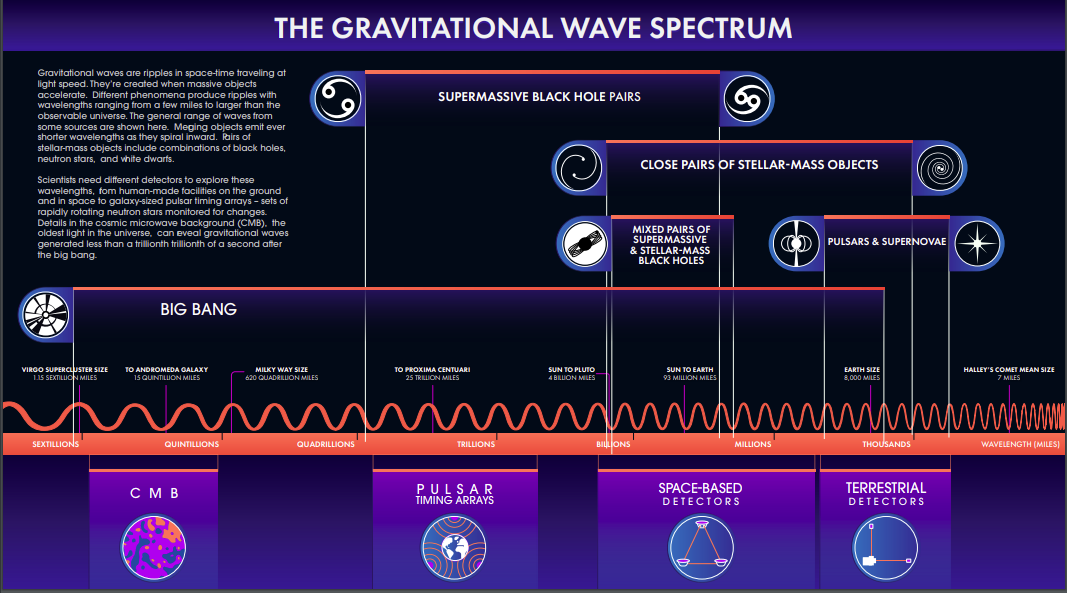
\includegraphics[width=4in]{images_/spectrum.png}
%     \caption{Gravitational-wave spectrum (credit: NASA)}
%     \label{fig:spectrum}
% \end{figure}

\section{Types of Gravitational Waves}
The classification of gravitational waves is based on the nature of their sources, the duration of their signals, and their waveform characteristics. There are several types of gravitational waves, each associated with different astrophysical sources and characteristics.
Gravitational waves are categorized into four main groups based on their sources:
% \vspace{0.2cm}

\subsection{Continuous Gravitational Waves} 
Continuous gravitational waves are emitted by fast-rotating, non-axisymmetric objects such as neutron stars. These objects may have small deformations on their surfaces, or they may be subject to internal instabilities that lead them to emit gravitational waves continuously over a long period. The source of continuous gravitational waves is usually a neutron star that is not exactly spherical. As it spins, any asymmetry in its mass distribution causes a periodic disturbance in spacetime, resulting in gravitational waves with a frequency proportional to its rotation rate. The gravitational waves produced are almost monochromatic, which means their frequency is generally consistent across time. This frequency may be somewhat altered by the star's interactions with its surroundings or change in its rotation.
\vspace{0.2cm}

\subsection{Compact Binary Inspiral Gravitational Waves} 

Compact binary inspiral gravitational waves thus results from inspiral and merger of two compact objects, neutron stars or black holes. These are some of the best-understood sources of gravitational waves. The sources are normally binary systems of neutron stars, black hole or both neutron star and black hole. These objects move in their orbits and in the process, they emit gravitational waves whereby they lose energy and hence their orbit shrinks and their orbital frequency increases. The produced gravitational waves have chirp signal in which both frequency and amplitude rise as the objects come closer. The waveform consists of three phases: Spiral, merger and ringdown. The inspiral is long, well modeled, and less energetic in contrast with the merger which is short, less modelled, and more energetic and the final ringdown, whereby the object created by the merger becomes stable.
\vspace{0.2cm}

\subsection{Stochastic Gravitational Waves} 
Stochastic gravitational waves are low-frequency gravitational waves from unresolved, disparate sources that overlap with each other: This background is similar to the cosmic microwave background radiation but for the gravitational waves. The stochastic background can have various astrophysical origins, such as a large number of low luminosity, unresolved mergers, core-collapse supernovae or the early universe; inflation, or cosmic strings. These sources contribute to a stochastic/ stochastic background of gravitational waves. Unlike the precise signals from individual events, the stochastic background is a random noise-like signal. Its detection is done with statistical measures other than the actual recognition of certain waveforms.
\vspace{0.2cm}

\subsection{Burst Gravitational Waves}
The burst gravitational waves are short-lived and transient signals that are due to sudden and catastrophic phenomena in the universe. Such events are often stochastic and might pose a problem in terms of modeling. Burst gravitational waves are normally associated with a core-collapse supernova, neutron star mergers, gamma-ray bursts, or another astrophysical catastrophe. These sources create ripples in the space-time fabric over a very short duration and therefore create a burst signal. The signal can have different duration, frequency, and amplitude depending on the source of the signal.

\section{Phase of Gravitational Waves}
The phase of a gravitational wave signal is the time evolution of the wave's oscillation. Gravitational wave signals can be divided into three phases (Fig \ref{fig:phase}):
   \begin{figure}[h]
        \centering
        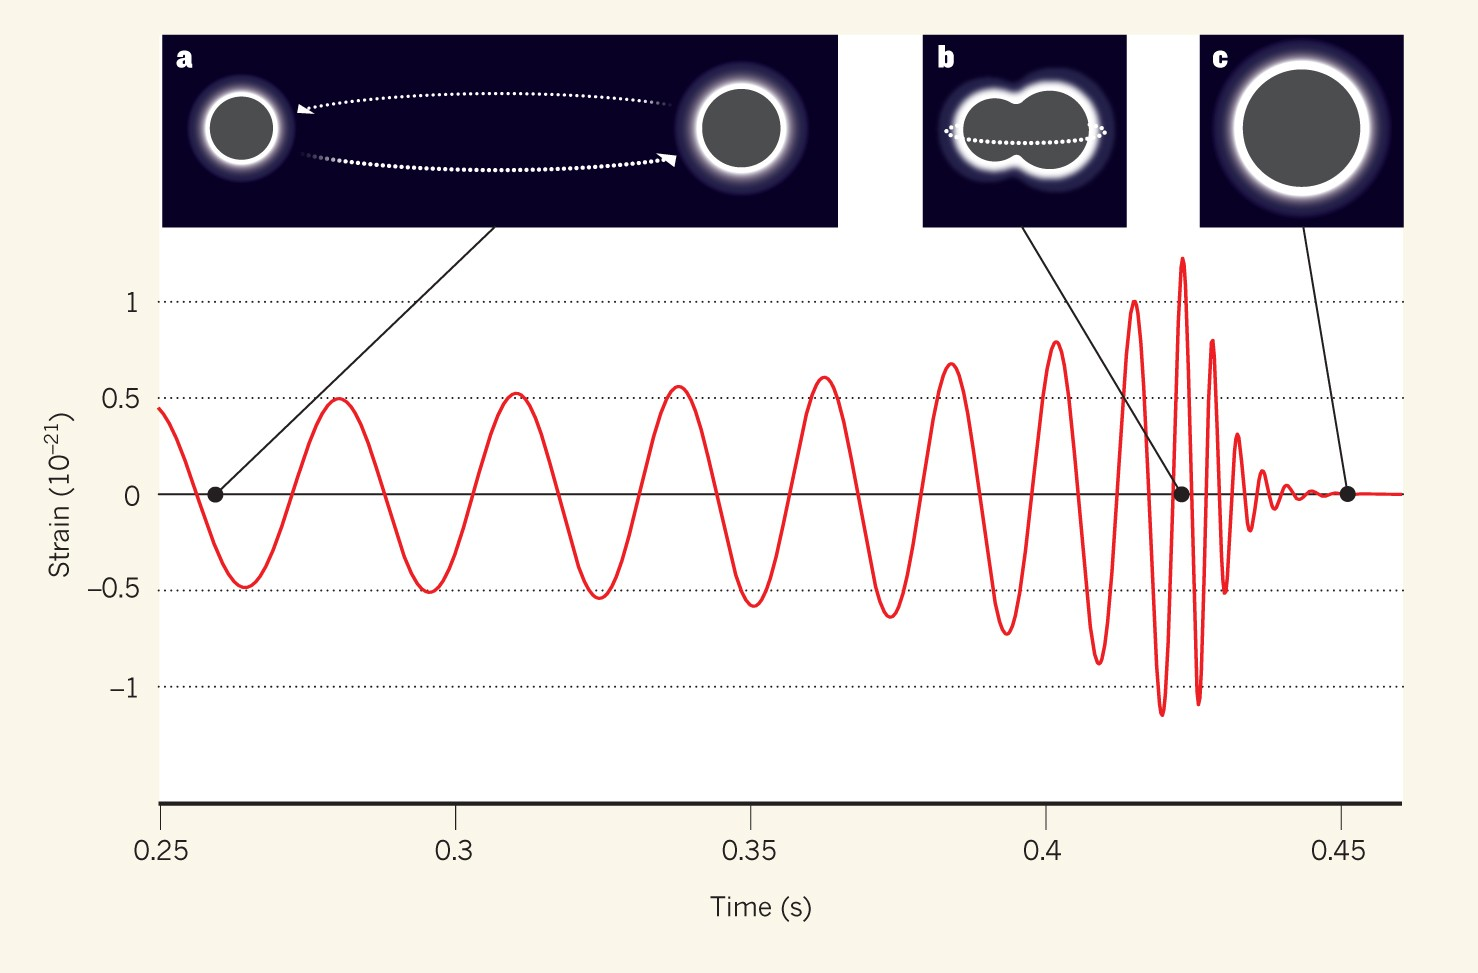
\includegraphics[width=4.5in]{images_/phase.jpg}
        \caption{A gravitational wave from merging black holes.(a) Inspiral Phase.(b) Merger Phase.(c) Ringdown Phase. Source: \citep{Miller2016}}
        \label{fig:phase}
    \end{figure}

    \subsection{Inspiral}
    The inspiral phase is the first phase of the gravitational wave signal in which two compact objects, such as neutron stars or black holes, gradually approach each other and orbit around their common center of mass because of the emission of gravitational radiation. In the inspiral phase, the GWS increases in both frequency as well as amplitude as the objects come closer to each other. This phase can continue for quite a long duration, especially in systems of lower mass, and is reasonably well explained by the post-Newtonian approximations of general relativity. When the objects are in orbit around each other the energy is radiated away in the form of gravitational waves and the separation of the objects reduces causing the orbits to become faster and the gravitational waves to become stronger. The rising of the frequency and the amplitude of the signal in a chirp-like manner is characteristic of this phase.
    
    \subsection{Merger}
    The merger phase is the most complex and the most violent phase of the gravitational wave signal and it is the phase where the two objects merge and form one object. The last phase of a binary’s life cycle is the merger phase as the frequency and amplitude rise steeply and steeply to the maximum values of the wave signal. This phase is very short and it can last for just a few milliseconds but the gravitational fields here are very strong and this is where general relativity’s nonlinear effects start to manifest themselves. It is within this process that the two objects’ gravitational fields are most intense and engage in a dance that is best explained through the numerical relativity simulations. The nature of the signal – frequency and its time variation – is defined by properties of the merging objects themselves, such as their masses, spins, and, in case the objects are neutron stars, the equation of state for these stars.
    
    \subsection{Ringdown} 
    The ringdown phase occurs after the merger and in essence, it is the period during which a newly-formed object settles down and becomes a black hole. This phase is characterised by exponential damping oscillations which are referred to as the quasinormal modes. The ringdown signal is a series of exponentially damped oscillations at a certain frequency which is determined by the mass and spin of the last formed black hole. These oscillations reduce in amplitude over time release of the rest of the distortions by the black hole.
    % \begin{figure}[h]
    %     \centering
    %     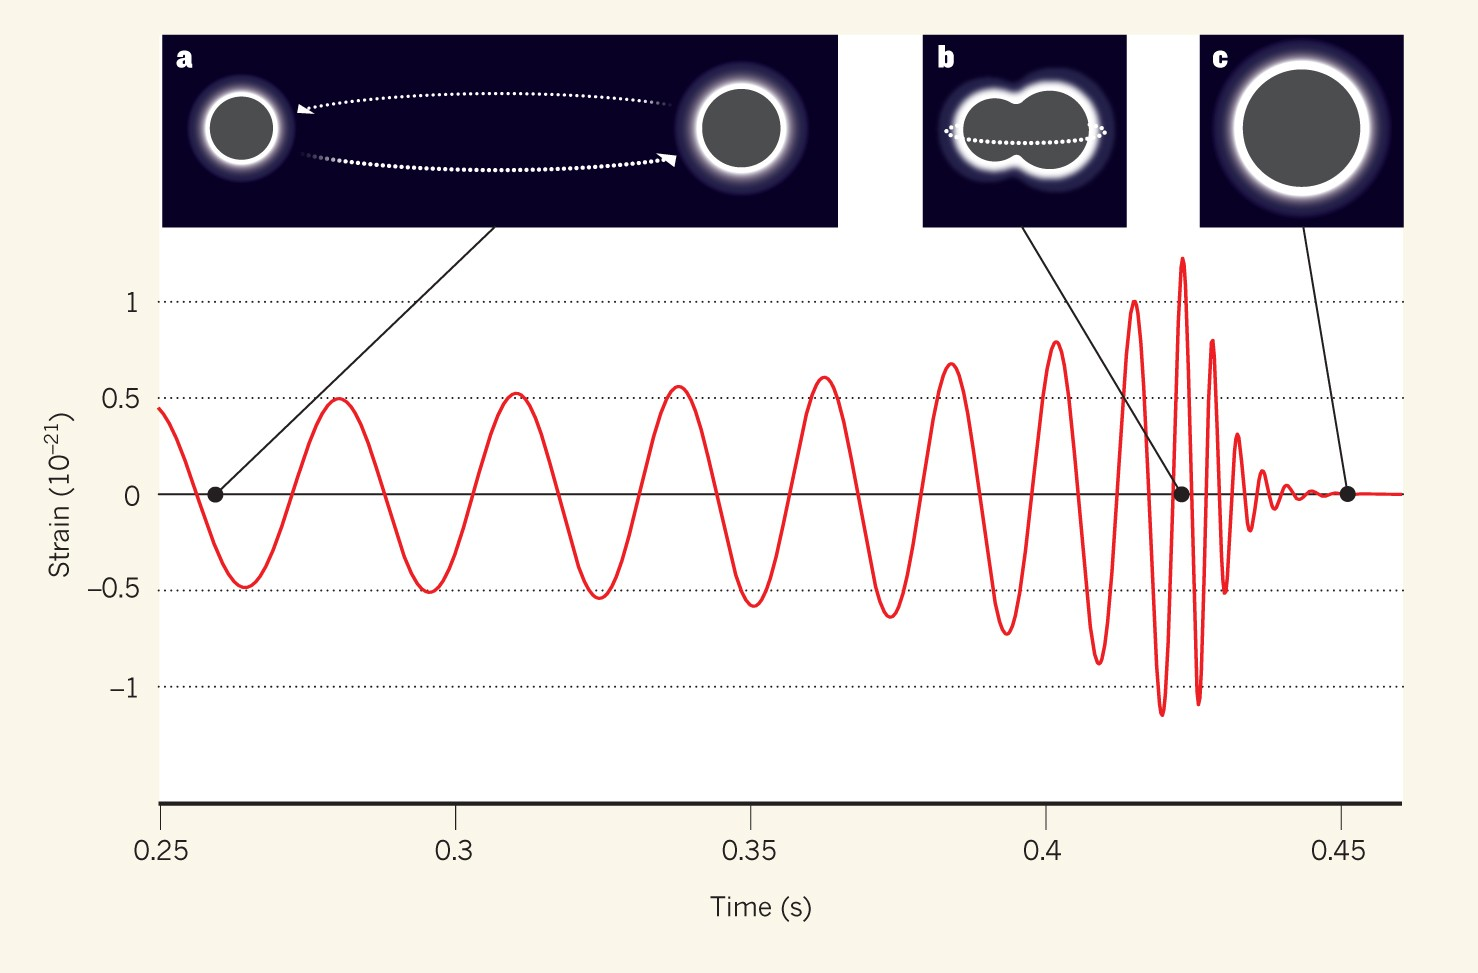
\includegraphics[width=4.5in]{images_/phase.jpg}
    %     \caption{A gravitational wave from merging black holes.(a) Inspiral Phase.(b) Merger Phase.(c) Ringdown Phase. Source: \citep{Miller2016}}
    %     \label{fig:phase}
    % \end{figure}
\section{Method of Gravitational Wave Detection}
Gravitational waves can be detected using two main methods: laser interferometry and pulsar timing arrays.
    
\begin{enumerate}
    \item \textbf{Laser Interferometry:} This method involves measuring tiny changes in the distance between two mirrors separated by a long distance (Fig: \ref{fig:interferometer}). When a gravitational wave passes through the detector, it stretches and squeezes space, causing slight changes in the mirror distance. Lasers and highly sensitive detectors are used to measure these changes with great precision. Laser interferometry detectors include LIGO, VIRGO, GEO600 and KAGRA.
    \begin{figure}
        \centering
        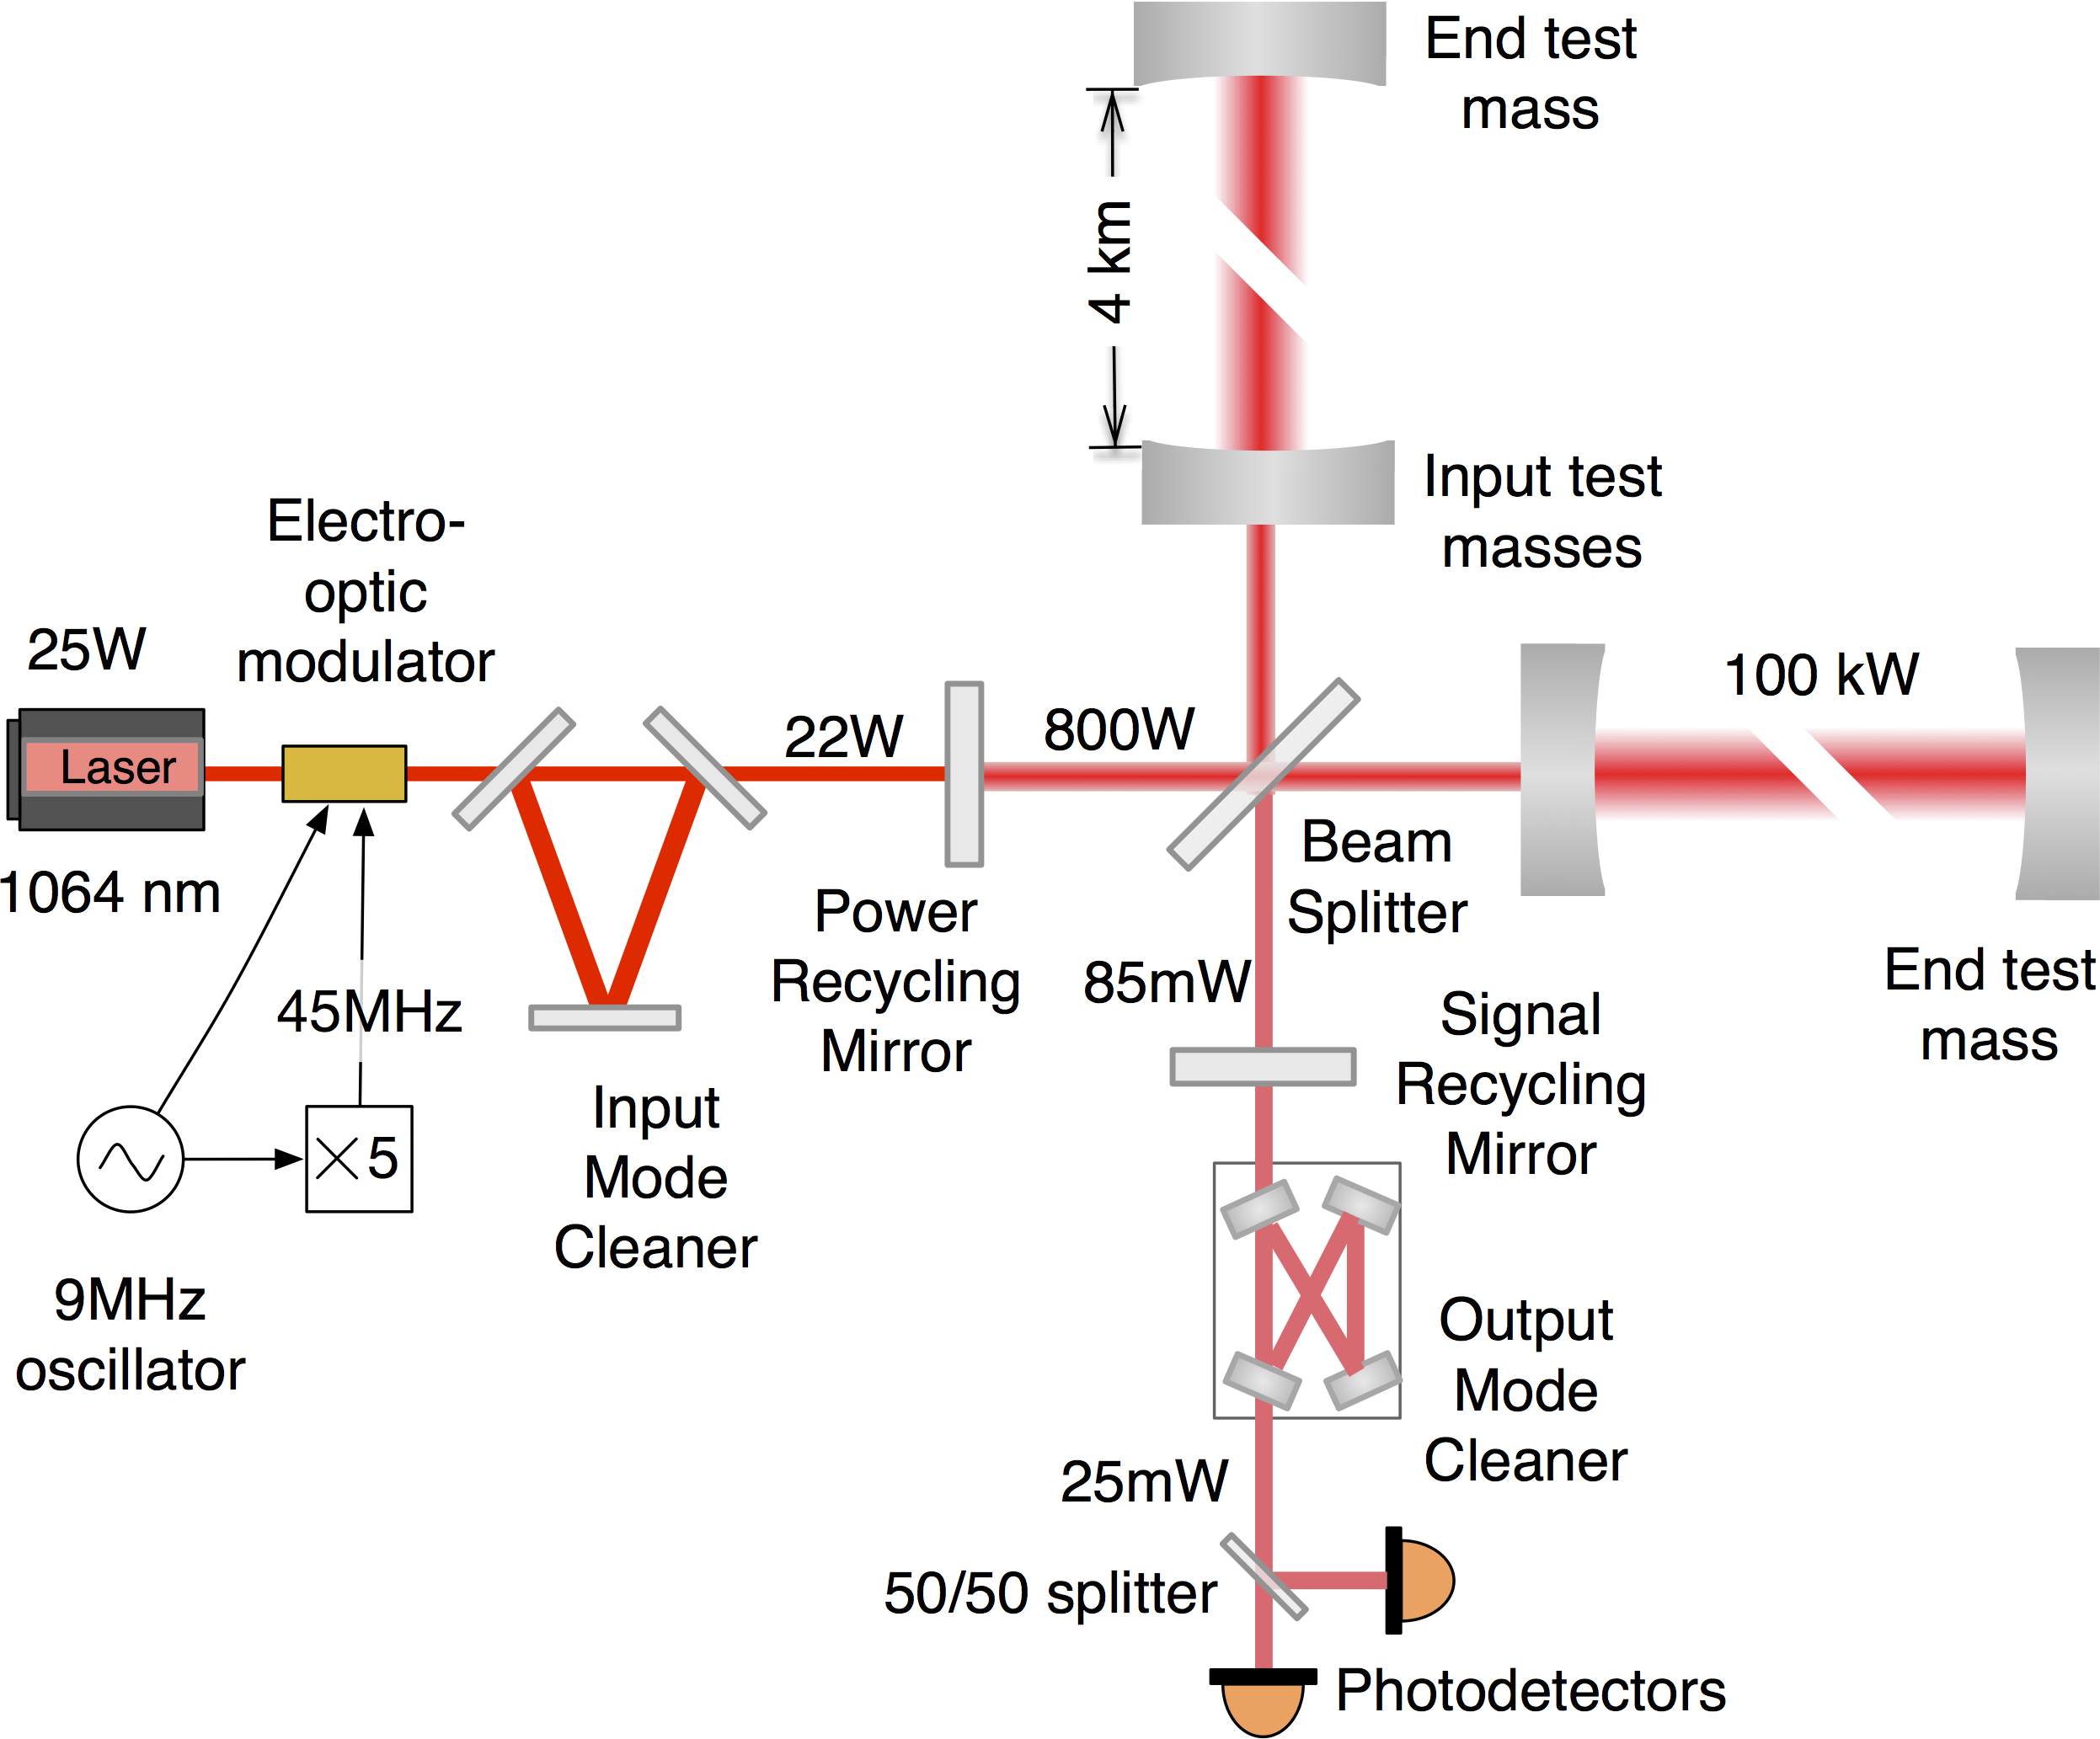
\includegraphics[width=0.65\linewidth]{images_/interferometer.png}
        \caption{LIGO's Interferometer. Source: \citep{PhysRevD.93.112004}}
        \label{fig:interferometer}
    \end{figure}
    
    \item \textbf{Pulsar Timing Arrays:} Pulsar timing arrays are networks of radio telescopes that are used to monitor the arrival times of pulses from millisecond pulsars. PTAs are less sensitive than laser interferometer gravitational wave detectors. However, PTAs can detect lower-frequency gravitational waves, which makes them well-suited for detecting gravitational waves from sources such as supermassive black hole mergers and cosmic strings. Examples are NANOGrav, EPTA and IPTA.
    
\end{enumerate}
% \section{Noises}
% "Noise" is unwanted and random fluctuations or signals that can obscure or mask the true gravitational wave signals. Some common sources of noise in gravitational wave detectors include:
%     \subsection{Seismic Noise} 
%     Ground vibrations caused by seismic activity, as well as other environmental factors like wind and temperature fluctuations, can introduce noise into the detector. To filter out these disturbances, the optical components are suspended to a series of several pendulums, each hanging from the above. 
%    \subsection{Thermal Noise} 
%    This source of noise in gravitational wave detectors is associated with the thermal vibrations of the mirrors and their suspensions. The steel wire that suspends the mirror is typically at room temperature, in thermal equilibrium with the surrounding environment. These thermal fluctuations can induce motion in the mirror, which, in turn, changes the length of the interferometer's arm.
%     \subsection{Quantum Noise}
%     Quantum mechanics imposes fundamental limits on the precision of measurements. Quantum noise arises due to the inherent uncertainty in position and momentum of particles. It can affect the accuracy of interferometric measurements used in many gravitational wave detectors.
%     \subsection{Shot Noise} 
%     Photon shot noise is the major limiting source of disturbance at frequencies above 200 Hz and results from the finite number of photons arriving at the photo-detector. Shot noise can be reduced by increasing the laser power. In order to be able to detect gravitational waves with frequency 100 Hz, the intensity of the laser would need to be of the order of 100 W, a value beyond the capability of any existing continuous laser.
%     \subsection{Mirror Coating Noise} 
%     The reflective coatings on mirrors used in interferometers can introduce noise when they fluctuate or deform, affecting the quality of the laser beam's reflection.
%     \subsection{Electromagnetic Interference (EMI)} 
%     External electromagnetic signals, including radio frequency interference (RFI) and electronic noise, can interfere with detector operations.
\section{Noises}

Noise refers to unwanted and random fluctuations or signals that can obscure or mask the true gravitational wave signals in detectors. The sensitivity and accuracy of gravitational wave detectors are significantly influenced by various types of noise. Understanding and mitigating these noise sources are crucial for accurate detections. Common sources of noise (Fig: \ref{fig:noises}) include:

\subsection{Seismic Noise} Seismic noise arises from ground vibrations caused by seismic activity, as well as environmental factors like wind, ocean waves, and human activities such as traffic and construction. These vibrations can be transmitted to the interferometer's components, particularly the mirrors, causing distortions that mimic or obscure gravitational wave signals. To reduce the impact of seismic noise, the optical components in detectors are suspended by multiple pendulums in a series, each hanging from the one above it. This sophisticated suspension system acts as a mechanical filter, isolating the mirrors from ground vibrations, especially at higher frequencies.

\subsection{Thermal Noise} Thermal noise is associated with the random thermal vibrations of the mirrors and their suspensions, which are typically made of materials like fused silica or steel. Even at room temperature, these materials experience microscopic vibrations due to thermal energy, leading to small, random movements of the mirrors. These movements can change the length of the interferometer's arms, introducing noise into the measurements. To mitigate thermal noise, gravitational wave detectors often operate at cryogenic temperatures, where thermal vibrations are significantly reduced. Additionally, advanced materials and coatings are used to minimize the mechanical losses that contribute to thermal noise.

\subsection{Quantum Noise} Quantum noise is a fundamental limitation imposed by quantum mechanics on the precision of measurements. It arises due to the Heisenberg uncertainty principle, which limits the simultaneous accuracy of position and momentum measurements. In the context of gravitational wave detectors, quantum noise primarily manifests as two effects: photon shot noise and radiation pressure noise. Photon shot noise, caused by the discrete nature of light, becomes significant at high frequencies, while radiation pressure noise, due to the fluctuating force exerted by photons on the mirrors, dominates at low frequencies. Techniques like quantum squeezing, where the quantum uncertainties are redistributed between variables, are employed to reduce quantum noise and enhance detector sensitivity.
\begin{figure}[h]
        \centering
        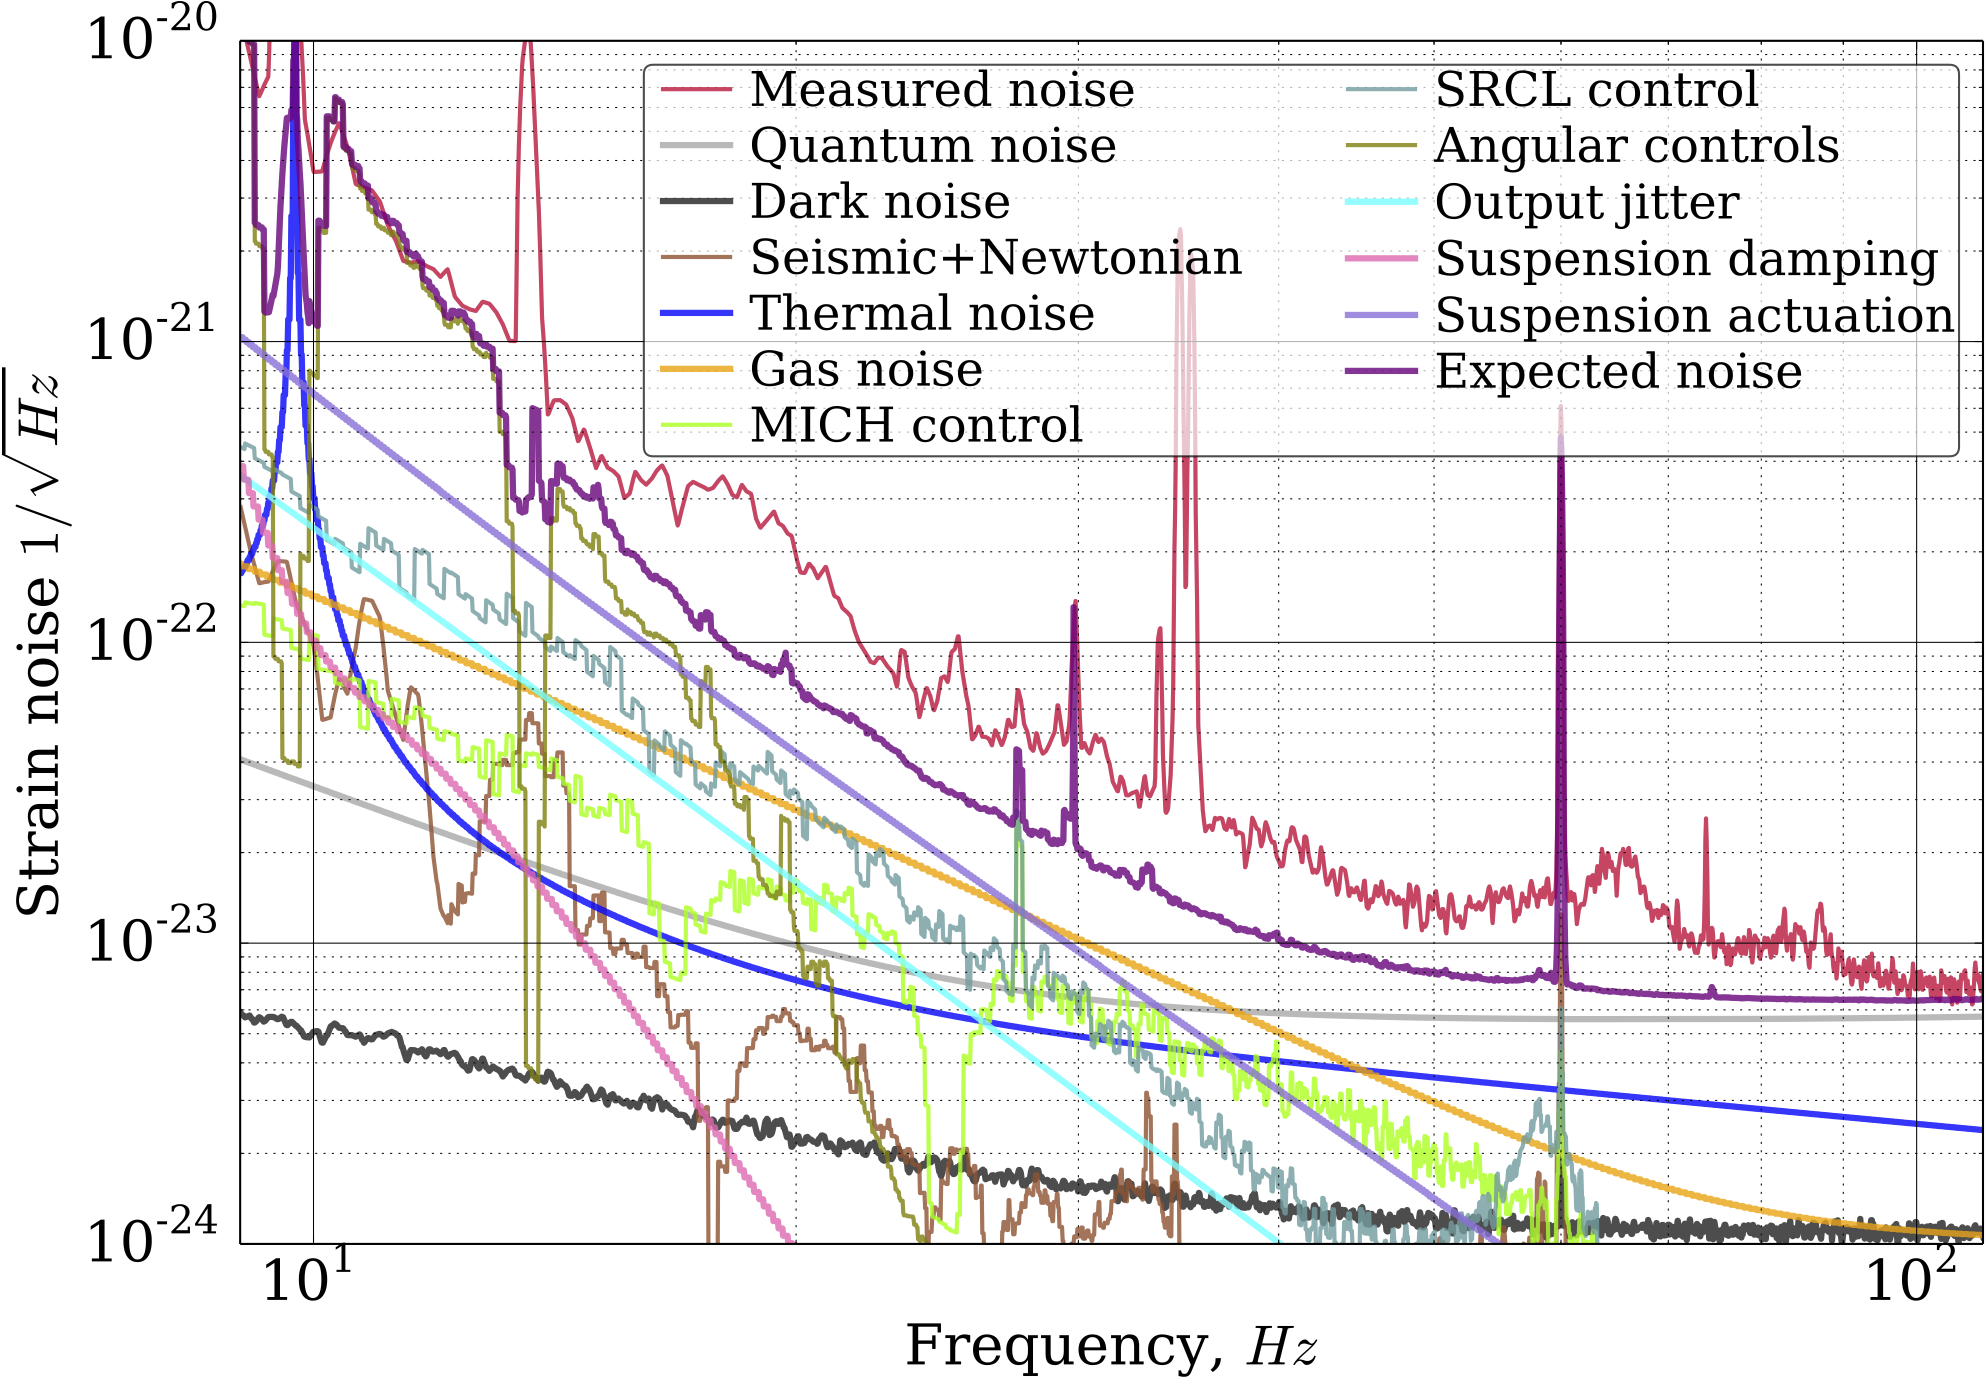
\includegraphics[width=4.5in]{images_/noise.png}
        \caption{ Accounting of sources of noise that combine to form the limiting sensitivity of the detectors. Source: \citep{PhysRevD.93.112004}}
        \label{fig:noises}
\end{figure}

\subsection{Mirror Coating Noise} Mirror coating noise is introduced by the reflective coatings on the mirrors used in interferometers. These coatings, typically made of materials like silica or tantala, are essential for reflecting the laser beam in the interferometer. However, thermal fluctuations and mechanical stress in the coating layers can cause them to deform or fluctuate, leading to noise in the reflected laser signal. This noise is particularly challenging to mitigate, as it is closely tied to the optical properties and thickness of the coatings. Research into advanced coating materials and techniques, such as crystalline coatings, is ongoing to reduce this type of noise.

\subsection{Electromagnetic Interference (EMI)} Electromagnetic interference is caused by external electromagnetic signals, such as radio frequency interference from communication devices, power lines, or electronic noise from nearby equipment. EMI can couple into the sensitive electronics of the detector, leading to spurious signals that mimic or obscure gravitational wave events. To protect against EMI, gravitational wave detectors are often housed in shielded environments with careful attention to grounding and cabling. Additionally, filters and isolation techniques are employed to prevent external electromagnetic signals from interfering with the detector's operations.
    % \begin{figure}[h]
    %     \centering
    %     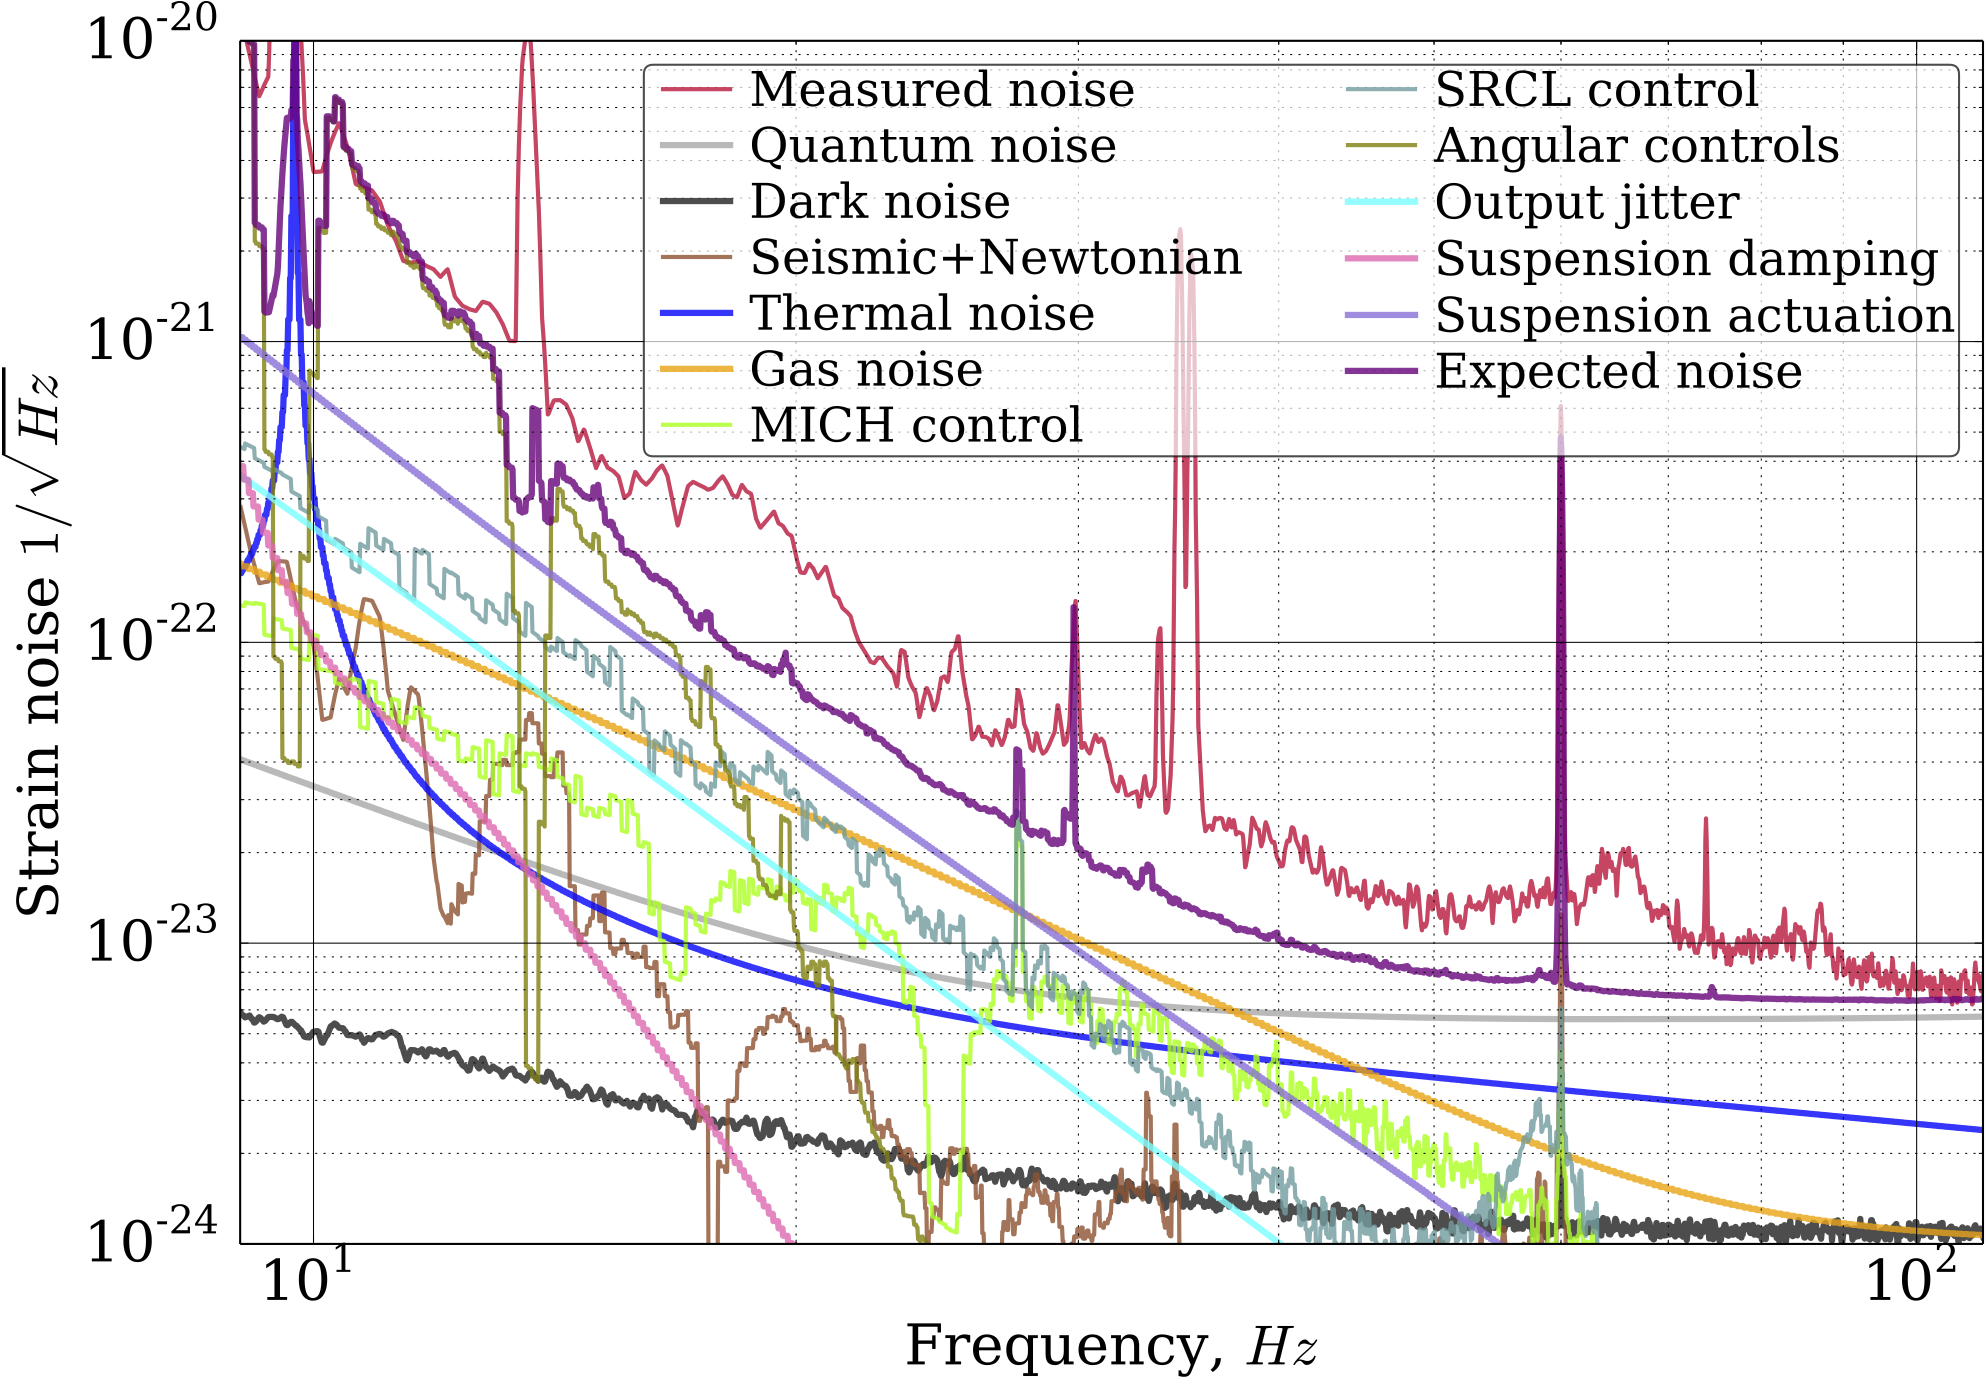
\includegraphics[width=4.5in]{images_/noise.png}
    %     \caption{ Accounting of sources of noise that combine to form the limiting sensitivity of the detectors. Source: \citep{PhysRevD.93.112004}}
    %     \label{fig:noises}
    % \end{figure}

\section{GW170817}
The Gravitational Wave Signal GW170817 was detected on August 17, 2017 by the Advanced LIGO and VIRGO Observatories \citep{2017ApJ...848L..12A}. GW170817 signal is produced from the collision of binary neutron stars. This GW signal is so unique that only 1.7 second after the detection of the signal, Fermi Gamma-ray Burst Monitor (GBM) and the Anticoincidence Shield for the Spectrometer for the International Gamma-Ray Astrophysics Laboratory (INTEGRAL SPI-ACS) detected a short $\gamma$-ray burst GRB 170817A \citep{Savchenko_2017}. For many decades, it had been suspected that these short $\gamma$-ray burst were produced by the merger of two neutron stars or a neutron star and a black hole. However, the detection of the GW signal with EM rays burst provides the first direct evidence of a link between these mergers and short $\gamma$-ray bursts called Kilonovae \citep{2017ApJ...848L..12A}. This unprecedented joint gravitational and electromagnetic observation provides insight into astrophysics, dense matter, gravitation, and cosmology.
\section{GW190521}
The Gravitational Wave Signal GW190521 was detected on May 21, 2019 by the LIGO and VIRGO detectors. It was produced from the merger of two intermediate mass black holes of each mass 85 and 66 $M_\odot$ with mass equivalent to 142 $M_\odot$. The remaining 9 $M_\odot$ were radiated away as energy in the form of gravitational waves \citep{abbott2020properties}. GW190521 defies stellar evolution predictions. The resulting black hole and at least one of its progenitors exceed the theorized 65 solar mass limit for stellar-born black holes, conclusively demonstrating that mergers of smaller black holes can populate the long-predicted mass gap between 65 and 142 $M_\odot$ \citep{abbott2020properties}
.
\section{GW190814}
The Gravitation Wave Signal GW190814 was detected on August 14, 2019 by the LIGO and VIRGO detectors. This signal originated from a pair of merging objects, one confirmed to be a giant black hole 23 times the Sun's mass. The other, clocking in at 2.6 $M_\odot$, remains a mystery – it could be either a fellow black hole but smaller, or a heavyweight neutron star \citep{abbott2020gw190814}.

\section{Significance of Gravitational Waves}
In astronomy and science in general, gravitational waves are extremely significant. They support the general theory of relativity postulated by Einstein, provide a new means of studying cosmic catastrophes, and allow an innovative tool for astronomy. Our knowledge of the extreme circumstances found in the universe has improved with the discovery of gravitational waves resulting from the mergers of neutron stars and binary black holes, ushering in a new age of multi-messenger astronomy. The features of huge astronomical objects, dark matter, and dark energy can all be better understood because to the extreme physics probed by these waves. Future discoveries of gravitational waves promise to solve more cosmic riddles while also stimulating scientific inquiry and technological advancement.
% \subsection{Motivation}
\section{Objectives}
This study sets out to investigate, via data analysis, the complex gravitational wave signals that arise from these remarkable collisions between celestial bodies.
\begin{itemize}
    \item  To verify that the gravitational waveforms seen in occurrences such as GW190521, and GW190814 are consistent with General Relativity's waveform predictions.
    \item  To use data analysis methods, including fourier transform, matched filtering, and  spectrogram to extract pertinent information from the gravitational wave signals.
    \item To propose possible paths for future research in understanding gravitational waves.
\end{itemize}
%end of objectives section
% The research project is deeply rooted in the transformative impact of gravitational wave astronomy on our understanding of the universe. Gravitational wave detectors, such as LIGO and Virgo, have ushered in a new era of exploration, enabling us to directly observe and interpret the gravitational whispers of the cosmos' most cataclysmic events. Among these celestial phenomena, binary systems composed of neutron stars and black holes stand as captivating and mysterious cosmic laboratories where the boundaries of our understanding are continually pushed to the extreme. I intend to study these events: GW170817, GW190521,and GW190814.
\vspace{0.4cm}

\textbf{GW170817}:
Studying GW170817 is crucial as it revolutionized astronomy. It was the first event observed in both gravitational waves and light, showcasing the power of using different methods to study space. This event also provided insights into neutron stars and confirmed how heavy elements like gold are formed in space, advancing our understanding of the cosmos.
\vspace{0.4cm}

\textbf{GW190521}:
GW190521, observed as a binary black hole merger, captured attention due to its unique characteristics. It featured an unusual mass ratio and is believed to have involved the formation of an intermediate-mass black hole. This event challenges conventional models of black hole evolution and dynamics, adding to the intrigue of our study.
\vspace{0.4cm}

\textbf{GW190814}:
GW190814 remains an intriguing enigma in the realm of gravitational wave astronomy. This event, which may have involved a neutron star-black hole binary, presents a unique challenge. Our aim is to uncover the true nature of the merger, further our understanding of compact object binaries, and potentially unveil new astrophysical phenomena.
\vspace{0.3cm}

Through these three events, the correlation among the gravitational wave events GW170817, GW190521, and GW190814 can be studied by comparing their waveforms, source properties, and astrophysical implications. Analyzing these events together allows us to identify commonalities and differences in the characteristics of binary systems, such as mass distributions, spins, and orbital dynamics. This comparative analysis can deepen our understanding of compact object mergers and their broader astrophysical context, enhancing our knowledge of extreme cosmic phenomena.

\newpage

\chapter{THEORETICAL BACKGROUND AND LITERATURE REVIEW}

\onehalfspacing

\section{Einstein Field Equations}
% General relativity asserts that the curvature of space-time causes gravity \citep{misner2017gravitation, thesis} \footnote{For Einstein paper, refer to \url{https://einsteinpapers.press.princeton.edu/}}. The presence of matter curves space-time and the curvature in turn determines the behaviour of matter. 
According to general relativity
% \footnote{For Einstein paper, refer to \url{https://einsteinpapers.press.princeton.edu/}}
, gravity is caused by the curvature of space-time \citep{misner2017gravitation}\citep{thesis}. Matter causes space-time to curve, and this curvature in turn affects how matter behaves.
The Einstein field equations for the gravitational field is:
\begin{equation}
    R_{\mu \nu}-\frac{1}{2} Rg_{\mu \nu} = 8\pi T_{\mu \nu},
    \label{eq:einstein}
\end{equation}
where $g_{\mu \nu}$ is the metric tensor of the four dimensional space-time and $T_{\mu \nu}$ is the stress energy tensor and $R$ is Ricci scalar also known as scalar curvature.\\
We are further interested in the study of gravitational radiation, which is considered as small perturbation that propagates over a flat space-time. Under these weak-field conditions, coordinate systems exist in which the metric's components may be broken down into
\begin{equation}
    g_{\mu \nu} = \eta_{\mu \nu} + h_{\mu \nu}, \hspace{1cm}  |h_{\mu \nu}|<< 1 \hspace{0.4cm}   
    \label{eq: metric}
\end{equation}
where $\eta_{\mu \nu}$ is the Minkowski metric that describes a space-time with no curvature. Such coordinates are particularly beneficial for solving equation \ref{eq:einstein}, which predicts gravitational waves.
% By applying ansatz \ref{eq: metric} to equation \ref{eq:einstein} and solving for the perturbative radiation field to first order in $h_{\mu \nu}$, we get the linearized Einstein equations
% \begin{equation}
%     - \partial^{\alpha}\partial_{\alpha}h'_{\mu \nu} -\partial^{\alpha}\partial^{\beta}h'_{\alpha \beta} +\partial^{\alpha}\partial_{\mu}h'_{\nu \alpha} +\partial^{\alpha}\partial_{\mu}h'_{\mu \alpha} = 16\pi T_{\mu \nu}
%     \label{eq: guage}
% \end{equation}
% on the field $h'_{\mu \nu}\equiv h_{\mu \nu} - \frac{1}{2} \eta_{\mu \nu}h_{\mu \nu}$. In the linear approximation this implies that two perturbations $h_{\mu \nu}$ and $h'_{\mu \nu}$ represent the same physical phenomenon if they are related by a transformation of the form
% \begin{equation}
%     h'_{\mu \nu} \rightarrow h_{\mu \nu} + \partial_{\mu}\xi_{\nu} + \partial_{\nu}\xi_{\mu},
%     \label{eq: arrow}
% \end{equation}
% where $\xi^{\alpha}$ is a vector field. 
% Without loss of generality, a field $\xi^{\alpha}$ can be found such that the following guage condition is verified
% \begin{equation}
%     \partial^{\alpha}h'_{\mu \alpha} = 0 \hspace{0.8cm} (Lorentz\hspace{0.1cm}guage), 
% \end{equation}
% in clear analogy with lorentz guage condition for the electromagnetic tensor $\partial_{\alpha}A^{\alpha}$. In the case of the linearized Einstein equations we need to impose the additional condition of being far away from the sources, so that the weak field condition \ref{eq: metric} is satisfied. This taken into account, equation \ref{eq: guage} in the lorentz guage simplifies to
% \begin{equation}
%     \partial^{\alpha}\partial_{\alpha}h'_{\mu \nu}  = 0 \quad (in\hspace{0.1cm}vacuum)
% \end{equation}
% Thus, we can always arrive at the guage
% \begin{equation}
%     h' = 0
% \end{equation}
% \begin{equation}
%     h'_{0i} = 0 \hspace{0.8cm} (i = 1,2,3) \quad (in\hspace{0.1cm}a\hspace{0.1cm}source free\hspace{0.1cm} region)
% \end{equation}
% \begin{equation}
%      h'_{00} = 0 \hspace{0.8cm} (if\hspace{0.1cm}no\hspace{0.1cm}sources\hspace{0.1cm}are\hspace{0.1cm}present\hspace{0.1cm}anywhere)
% \end{equation}
% which is referred to as radiation guage. In this transverse-traceless guage $h'_{\mu \nu} = h_{\mu \nu}$.


The Einstein field equations in vacuum that are located far from the field's source have the following form \citep{thesis}
\begin{equation}
    \left(-\frac{\partial^2}{\partial t^{2}} + \nabla^{2}\right)h_{\mu \nu} = 0,
\end{equation}
a gravitational wave equation that gives the plain wave solution
\begin{equation}
    h_{\mu \nu} = a_{\mu \nu}.e^{ik_{\alpha}x^{\alpha}},
    \label{eq: plane}
\end{equation}
where $\alpha_{\mu \nu}$ is a four-dimensional symmetric tensor containing the amplitude of the different components of the wave and $k^{\alpha}$ is the wave vector. 

% If we further orient the direction of propagation of the wave along the z-axis so that $k^{\alpha} = (\omega,0,0,\omega)$ then $a_{\alpha z} = 0$ for all $\alpha$.  These condition reduce the number of independent components of $a_{\mu \nu} $ from ten to only two \\
% \begin{equation}
%     a_{\mu \nu} = 
%     \begin{pmatrix}
%     0 & 0 & 0 & 0\\
%     0 & a_{xx} & a_{xy} & 0\\
%     0 & a_{xy} & -a_{xx} & 0\\
%     0 & 0 & 0 & 0\\
% \end{pmatrix}


For the perturbative field, the source-free, linearized Einstein equations have a final form of
\begin{equation}
    h_{\mu \nu} = 
    \begin{pmatrix}
         0 & 0 & 0 & 0\\
         0 & h_{+} & h_{\times} & 0\\
         0 & h_{\times} & -h_{+} & 0\\
         0 & 0 & 0 & 0\\
    \end{pmatrix}
    .e^{i\omega(z-t)},
\end{equation}
with $h_{+}$ and $h_{\times}$ representing the two polarization states. A gravitational wave can be written as a linear combination of the \textit{plus} and \textit{cross} components $h = h_{+}\hat{e}_{+} + h_{\times}\hat{e}_{\times}$ in the orthonormal basis of vectors
\begin{equation}
    \hat{e}_{+} = 
    \begin{pmatrix}
        1 & 0\\
        0 & -1\\
    \end{pmatrix} \quad
    \hat{e}_{\times} = 
    \begin{pmatrix}
        0 & 1\\
        1 & 0\\
    \end{pmatrix}
\end{equation}
% Rotation of the x- and y-axes in the transverse plane by an angle $\psi$ change the polarization components in the follow way
% \begin{equation}
%     \begin{aligned}
%         h'_{+} = h_{+}\cos{2\psi} + h_{\times}\sin{2\psi}\\
%          h'_{\times}  = -h_{+}\sin{2\psi} + h_{\times}\cos{2\psi},
%     \end{aligned}    
% \end{equation}
% which indicates that general relativistic gravitational waves have spin two.

\section{Effects of Gravitational Waves on Test Particles}
In the background Lorentz frame, consider two free falling particles A and B.
Let us denote the connecting vector $\xi^{\alpha}$ between points A and B. For the 4-velocity $u^{\alpha}$, free particles follow the geodesic equation \citep{misner2017gravitation}\citep{thesis}\citep{Generalrelativity}
\begin{equation}
    u^{\alpha}\nabla_{\alpha}u^{\beta} = 0
\end{equation}
The vector $\xi^{\alpha}$ has a second derivative that is non-zero in a curved space-time, suggesting an acceleration between particles A and B. We will get the result
\begin{equation}
    \frac{d^{2}\xi^{i}}{dt^{2}} = \frac{1}{2} \frac{d^{2}h_{ij}}{dt^{2}} \xi^{j}
    \label{eq: stretch}
\end{equation}
where i,j = 1,2 representing the x- and y-directions.
\begin{figure}[h]
    \centering
    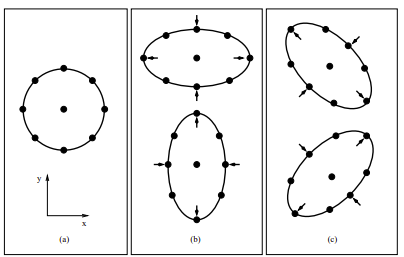
\includegraphics[width=3in]{images_/stretch.png}
    \caption{Effect of the two polarizations of a gravitational wave propagating through a ring of test particles. Source: \citep{doi:10.1142/9789813141766_0001} }
    \label{fig: stretch}
\end{figure}
A ring of particles at rest on the xy-plane in an initial wave-free region of space-time encounters a gravitational wave traveling in the $z$ direction. The arrival of the wave alters the proper separation between the particles. The \textit{plus} polarization of the wave stretches and squeezes the ring along the x- and y-axes, oscillating between the shapes seen in panel (b) of figure \ref{fig: stretch}.\\
Once we understand the effects of a gravitational wave passing on a pair of test particles, we could develop tools to detect that effect, which could involve a laser and an interferometer of arm's length L. Assuming that the gravitational wave's wavelength is substantially larger than the interferometer's size, the equation integration becomes simpler equation \ref{eq: stretch}
\begin{equation}
    \delta x = \frac{h_{xx}}{2}x, \hspace{0.5cm} \delta y = \frac{h_{yy}}{2}y.
\end{equation}
When a gravitational wave passes along the z-direction with polarization $h_{xx} = -h_{yy} = h_{+}(t)$, the change in proper distance and the phase difference between the two beams at the origin are
\begin{equation}
    \frac{\delta L(t)}{L} = h_{+}(t), \hspace{0.8cm} \Delta \phi = 2\pi \frac{L}{\lambda}h_{+}(t)
\end{equation}
The difference in phase between the beams recombining at the beam splitter is proportional to
\begin{equation}
    h(t) \propto \delta (\Delta \phi) \equiv F_{+}h_{+}(t) + F_{\times}h_{\times}(t),
\end{equation}
where $F_{+}$ and $F_{\times}$ are the antenna patterns of the detector. The quantity $h$ is the \emph{gravitational wave strain}.\\
The spatial variation of the gravitational wave in the arms of the interferometer is considered to be insignificant in this derivation. We do not account for the temporal fluctuation of $h(t)$ during the brief interval $\approx 2L$ that the light takes to go back and forth to the mirror. 


\section{Gravitational Waves Of Binary Stars}
Compact objects like neutron stars or black holes that are orbiting each other and are bound together by gravity go through a process called coalescence in which some of their energy is released as gravitational radiation \citep{Blanchet_2002}\citep{coalesence}\citep{thesis}. In gravitational-wave astronomy, these merging binaries are particularly important because they are promising candidates for first detection.

The gravitational wave emanating from pairs of black holes or neutron stars can be described using various analytical and numerical theoretical approaches. During the inspiral phase, the binary's orbital frequency increases as they lose energy to gravitational waves, which can be described by the post-Newtonian approximation. The emitted gravitational wave strain \( h(t) \) \citep{Blanchet_2002}\citep{Hughes_2009} is given by:

\begin{equation}
h(t) = \frac{4G\mu}{c^2R} \left( \frac{G\mathcal{M}}{c^3} \right)^{5/3} f(t)^{2/3} \cos[\phi(t)]
\end{equation}

where:
\begin{itemize}
    \item \( G \) is the gravitational constant,
    \item \( \mu \) is the reduced mass of the binary system,
    \item \( c \) is the speed of light,
    \item \( R \) is the distance to the binary system,
    \item \( \mathcal{M} = (\mu)^{3/5}M^{2/5} \) is the chirp mass, with \( M \) being the total mass,
    \item \( f(t) \) is the gravitational wave frequency,
    \item \( \phi(t) \) is the phase of the wave.
\end{itemize}

The frequency evolution of the gravitational wave, \( f(t) \), as the binary inspirals, can be described by:

\begin{equation}
f(t) = \frac{1}{\pi} \left( \frac{5}{256} \frac{1}{\tau(t)} \right)^{3/8} \left( \frac{c^3}{G\mathcal{M}} \right)^{5/8}
\end{equation}

where \( \tau(t) \) is the time to coalescence.

As the binary reaches the merger phase, numerical relativity simulations are employed to solve the full Einstein field equations, providing accurate descriptions of the gravitational waveforms during the merger and ringdown phases. The merger phase generates a strong gravitational wave signal as the two compact objects collide, forming a single, more massive object.

The ringdown phase follows, where the newly formed object emits gravitational waves as it settles into a stable state. This phase can be described using the quasi-normal modes of the remnant object, typically modeled as a damped sinusoidal wave:

\begin{equation}
h(t) = A e^{-t/\tau} \cos(2\pi f_{\text{ring}} t + \phi)
\end{equation}

where:
\begin{itemize}
    \item \( A \) is the amplitude,
    \item \( \tau \) is the damping time,
    \item \( f_{\text{ring}} \) is the ringdown frequency,
    \item \( \phi \) is the phase.
\end{itemize}

These equations and theoretical models are critical for predicting the gravitational wave signals from coalescing binaries, enabling their detection and analysis in gravitational-wave astronomy \citep{Blanchet_2002}.


\section{Literature Review}
A century ago, Einstein proposed gravitational waves as spacetime ripples resulting from mass acceleration, although doubts lingered. Detecting these waves posed a formidable challenge spanning decades. Additionally, Einstein's theory predicted the existence of black holes—cosmic entities formed through intense spacetime curvature. The understanding of black holes became closely linked with the pursuit of gravitational wave detection. It wasn't until the late 1950s that calculations began to solidify the belief in the existence of gravitational waves. Finally, in the 1970s, indirect evidence emerged when astronomers observed a double pulsar system PSR 1913+16 \citep{1975ApJ...195L..51H} for which measurements of the decay of the orbital period with time are consistent with the energy losses expected for gravitational-wave emission, confirming the energy loss predicted by gravitational wave theory.
\vspace{0.2cm}

On September 14, 2015, the LIGO collaboration made history by detecting GW150914, the first gravitational wave event. This monumental discovery, results from the merger of two massive black holes \citep{abbott2016observation}.
\vspace{0.2cm}

Further, On August 17, 2017, the Advanced LIGO and Advanced VIRGO detectors observed GW170817, marking the first binary neutron star inspiral detection. The signal had a high signal-to-noise ratio 32.4 and a rare false-alarm rate. It suggested component masses between 0.86 and 2.26 $M_\odot$ or 1.17 to 1.60 $M_\odot$ when considering neutron star spins. The total system mass was estimated at 2.74 $M_\odot$. The event was localized within 28 square degrees, the closest such localization. It was associated with gamma-ray burst GRB 170817A, linking neutron star mergers to short gamma-ray bursts \citep{2017ApJ...848L..12A}.
\vspace{0.2cm}

In May 2019, the Advanced LIGO and Advanced VIRGO detectors observed the gravitational wave event GW190521 \citep{abbott2020gw190521}\citep{martin2020gw190521}, characterized by a high signal-to-noise ratio and a low estimated false-alarm rate. This event is believed to result from the merger of two black holes, with estimated masses of approximately 85-66 $M_\odot$. The primary black hole's mass is likely within a range produced by pair-instability supernova processes. The remnant black hole has an estimated mass of about 142 $M_\odot$, classifying it as an intermediate mass black hole. The remaining 9 $M_\odot$ were radiated away as energy in the form of gravitational waves \citep{abbott2020properties}\citep{abbott2020gw190521}. The source of GW190521 is located at a luminosity distance of $5.3 Gpc$, corresponding to a redshift of 0.82. The inferred rate of similar black hole mergers in the universe is approximately 0.13 $Gpc^{-3} yr^{-1}$. These findings provide valuable insights into black hole mergers and their astrophysical implications.
\vspace{0.2cm}

GW190814, observed on August 14, 2019, \citep{abbott2020gw190814} by LIGO and VIRGO, represents a significant gravitational wave event. It involves a compact binary coalescence featuring an unequal mass ratio, with a black hole ranging from 22.2 to 24.3 $M_\odot$ and a compact object between 2.50 and 2.67 $M_\odot$. The signal boasted a high signal-to-noise ratio and was localized to a distance of 241 Mpc \citep{abbott2020gw190814}\citep{staff2020mysteryobject}\citep{staff2020gw190814}. This event challenges current astrophysical models due to its unique mass ratio, component masses, and estimated merger rate density, which ranges from 1 to 23 $Gpc^{-3} yr^{-1}$. Furthermore, tests of general relativity revealed no deviations, confirming its predictions for higher-multipole emission. The origin and characteristics of GW190814 raise intriguing questions in the field of compact-object binary formation \cite{abbott2020gw190814}\citep{staff2020mysteryobject}\citep{staff2020gw190814}.


\newpage

\chapter{METHODOLOGY}
\onehalfspacing

In this section, We outline the methodologies and techniques we intend to employ for the gravitational wave data analysis.

\section{Data Acquisition}
This study makes use of publicly available datasets from the LIGO and VIRGO collaborations, which offer comprehensive details on gravitational wave occurrences that have been identified. These datasets are obtained by using gwosc and gwpy python packages. GWpy \cite{gwpy} is a collaboration-driven Python package providing tools for studying data from ground-based gravitational-wave detectors. The package integrates seamlessly with common scientific libraries like NumPy, SciPy, and Matplotlib, making it a powerful tool in the field of gravitational wave astronomy.

\begin{lstlisting}[language=Python, caption=Downloading data from GWOSC using GWPY, label=code:strain]
from gwosc import datasets
from gwpy.timeseries import TimeSeries
gps0 = datasets.event_gps("GW170817") # --> 1187008882.4
gps1 = datasets.event_gps("GW190521") # --> 1242442967.4
gps2 = datasets.event_gps("GW190814") # --> 1249852257.0 
# GW170817,  duration of 1024 seconds at 4096 sample rate
ldata0 = TimeSeries.fetch_open_data('L1', int(gps0)-512, int(gps0)+512, cache=True)#Livingston
hdata0 = TimeSeries.fetch_open_data('H1', int(gps0)-512, int(gps0)+512, cache=True) #Hanford 
vdata0 =  TimeSeries.fetch_open_data('V1', int(gps0)-512, int(gps0)+512, cache=True) #VIRGO
# GW190521
ldata1 = TimeSeries.fetch_open_data('L1', int(gps1)-512, int(gps1)+512, cache=True)
hdata1 = TimeSeries.fetch_open_data('H1', int(gps1)-512, int(gps1)+512, cache=True) 
vdata1 =  TimeSeries.fetch_open_data('V1', int(gps1)-512, int(gps1)+512, cache=True) 
# GW190814
ldata2 = TimeSeries.fetch_open_data('L1', int(gps2)-512, int(gps2)+512, cache=True)
hdata2 = TimeSeries.fetch_open_data('H1', int(gps2)-512, int(gps2)+512, cache=True) 
vdata2 = TimeSeries.fetch_open_data('V1', int(gps2)-512, int(gps2)+512, cache=True) 
\end{lstlisting}

% \subsection{Data Preprocessing}
After the data from each GW event detected by L1, H1, and V1 have been extracted using the APIs of the gwosc and gwpy python packages, they are preprocessed for cleaning and preparation for further analysis. This preprocessing includes steps such as performing FFT, windowing, cleaning, and more.

\section{ Discrete Fourier Transform (DFT)}
 Discrete Fourier Transform (DFT)
 % \footnote[1]{For more understanding of signal processing, refer to \cite{lyons2004understanding,proakis2007digital}}
 is a mathematical technique used to convert a discrete time-domain signal into its frequency-domain representation. It involves computing the complex exponential sum of the signal and its frequency components. DFT converts a sequence of $N$ complex number
 % \footnote[1]{in practise, time domain signal/sample signal $x_{n}$ are real but outputs are complex}
 $x_{0},x_{1},....,x_{N-1}$ to a new sequence of $N$ complex number,
 \begin{equation}
     X_{k} = \sum_{n=0}^{N-1} x_{n}.e^{-2\pi ikn/N}
 \end{equation}
 for $0\leq k\leq N-1$.\\
 The $x_{n}$ are thought of as the values of a signal, at equally spaced time interval. The output $X_{k}$ is a complex number which encodes the amplitude and phase of a sinusoidal wave with frequency $\frac{k}{N}$ cycles per time unit. The frequency corresponding to  $k$ is given by $f_{k} = k.F_{s}/N$, where $F_{s}$ is the sampling frequency. For more understanding of signal processing, see \cite{lyons2004understanding}\citep{proakis2007digital} 
 
The inverse DFT $"x_{n}"$ is:
\begin{equation}
    x_{n} = \frac{1}{N} \sum_{k=0}^{N-1} X_{k}.e^{2\pi ikn/N}
\end{equation}
The traditional implementation of the DFT has a time complexity of $O(N^2)$, where N is the number of data points. This means that the computation time increases quadratically with the size of the input.

However, thanks to the Fast Fourier Transform (FFT) algorithm \cite{cooley1965algorithm}, the computational cost of computing the DFT can be significantly reduced. The FFT is an efficient algorithm for calculating the DFT, and its time complexity depends on the specific implementation but is typically $O(N.log N)$. 
FFT can be performed on our data using the \textit{numpy} or \textit{scipy} modules in Python. The gwpy module \cite{gwpy} has a built-in FFT method with ready-made parameters. However, we used the both scipy and numpy module to better understand the FFT process by setting the appropriate parameters ourselves.

% \footnote{\url{https://dspillustrations.com/pages/posts/misc/spectral-leakage-zero-padding-and-frequency-resolution.html}}
\section{Windowing}
The FFT operates under the assumption that the data is periodic. This assumption can result in the edges of the data appearing as discontinuities when transformed. Therefore, we need to apply a window function to our time-domain data before transforming it into the frequency domain.

Windowing in signal processing involves multiplying a signal by a mathematical function known as a window function. This function is typically zero-valued outside of a specific interval and smoothly tapers at its edges. The primary purpose of windowing is to select a portion of a signal for analysis while reducing the disruptive effects of discontinuities at the signal's edges. Windowing is especially important in spectral analysis, such as when performing a fast Fourier transform, to mitigate spectral leakage, which occurs when energy from one frequency bin spreads to others due to non-periodic signals or incompatible window lengths \cite{lyons2004understanding}\citep{proakis2007digital}. 

We employed the Hann function (see code \ref{code:Hann}) as a window to our data. The Hann function, also known as the Hann or Hanning window, is a mathematical function used in signal processing to reduce spectral leakage during Fourier transform analysis. It is defined as:
\begin{equation}
    w(n) = 0.5 \left(1 - \cos\left(\frac{2\pi n}{N-1}\right)\right)
\end{equation}
for \( n = 0 \) to \( N-1 \), where \( N \) is the length of the window. The Hann function has a smooth, cosine-like shape that tapers to zero at the edges, helping to minimize discontinuities in the signal, which can otherwise spread energy into adjacent frequency bins in the Fourier transform. 

By reducing abrupt transitions and ensuring continuity, this tapering also aids in maintaining signal integrity. Furthermore, compared to other window functions, the Hann window offers reasonable frequency resolution while maintaining side lobe levels at lower levels by striking a compromise between main lobe width and side lobe levels (Fig \ref{fig:hannFunction})

\begin{lstlisting}[language=Python, caption=Hann Windows Function of data size, label=code:Hann]
#from scipy.signal import get_window()
import numpy as np
import matplotlib.pyplot as plt
plt.plot(np.hanning(ldata0.size)) #example: same data size
# plt.plot(get_window('hann', ldata0.size))  
plt.xlabel("x")
plt.ylabel("Hann function")
plt.grid(False)
plt.show()
\end{lstlisting}
\vspace{0.7cm}
\begin{figure}[h]
        \centering
        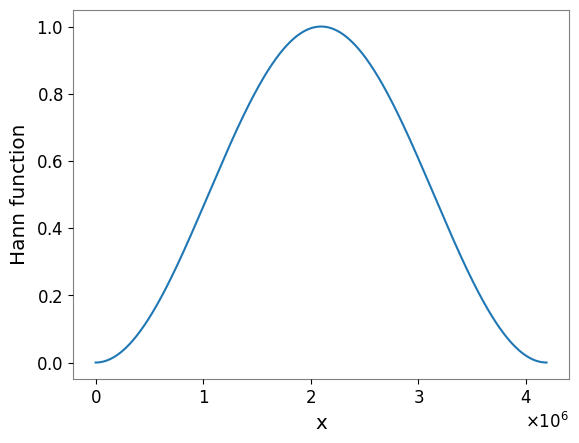
\includegraphics[width=2.5in]{images_/nphanning.png}
        \caption{ Hann function of data size}
        \label{fig:hannFunction}
\end{figure}
\vspace{0.5cm}
Then, we performed the FFT on our windowed signal (see code \ref{code:fft}) and obtained the absolute value of the output by using numpy module.
\begin{lstlisting}[language=Python, caption=FFT on windowed signal using numpy, label=code:fft]
import numpy as np
# multiply actual data with windows function
def window_data(data, function):
  wf = get_window(function,data.size)  #function parameter,a string, as window function
  wd = data*wf
  return wd
# perform fft on windowed data(wdata)
def fft_on_windowedsignal(wdata):
  dft = np.fft.rfft(wdata, n=wdata.size)/wdata.size
  dft[1:] *= 2.0
  return dft
# calculate the absolute values of return fft
def fftabsolutevalue(fftdata):
   return np.abs(fftdata)
\end{lstlisting}
All Fourier coefficient amplitudes are doubled by the line 4 in above code, with the exception of the zero frequency component (DC component). The rfft function only returns the positive frequency terms of the DFT, and for real-valued input signals, the energy of the negative frequency terms is implicitly included in these positive terms. That's why we had to modify the dft.

\section{Power Spectral Density}
The power (energy per unit time) of a signal as a function of frequency is measured by the Power Spectral Density.
In order to differentiate real GW signals from noise, it is firstly necessary to be able to characterize noise behavior in great detail across a range of frequencies. Understanding the PSD in its entirety allows us to maximize the signal-to-noise ratio and improve GW signal recognition with the use of signal processing techniques like matched filtering.
Taking the square root of the above calculation in PSD allows us to express the result more conveniently as an amplitude rather than as a power. The quantity obtained is referred to as the signal's Amplitude Spectral Density. 

We performed ASD on windowed data using gwpy module (see code \ref{code:asd}) which has asd() method \cite{gwpy} available.
\begin{lstlisting}[language=Python, caption=Amplitude Spectral Density using gwpy, label=code:asd]
# using gwpy as ldata0 is a timeseries, output by gwpy
amplitude_sd0 = ldata0.asd(fftlength=4, method="median")
# so on for other data
#fftlength =4 (mostly used), the duration(s) of the data used to estimate each FFT
# the method used to average them. 
\end{lstlisting}
\section{Spectogram}
The frequency content of a signal over time is shown visually in a spectrogram. This two-dimensional graphic shows the distribution of the signal's energy over time (horizontal axis) along different frequencies (vertical axis). The amplitude of the signal is encoded in color intensity at each time-frequency point; cooler colors denote a weaker signal presence, and brighter colors indicate a stronger signal presence. Spectrograms provide important information about the fundamental frequency, harmonic components, and non-stationary behavior of the signal.
However, without having much prior information of the signal morphology, we can apply a unique filter known as a Q-transform to generate a time-frequency representation of our data. This representation enables us to identify features at different frequencies and how they change over extremely short timeframes. Gwpy has builtin spectogram/spectogram2() and q-transform() method (see Appendix \ref{code1}). We adjusted these method's parameter such as frequency range, q-range and outseg to better resolve the feature.

\section{Matched Filtering}
A key method for detecting GWs is matched filtering, which is intended to spot faint signals in noisy data. We used PYCBC python library to perform data extraction, highpass filtering and resampling stages, generating waveform and matched filtering (see Appendix \ref{code2}). First, a set of theoretical waveform templates depicting our extracted gravitational wave signals of GW170817, GW190521 and GW190814  were created. These general relativity and numerical simulation-based templates were used as models to compare our data. Preprocessing was applied to the gathered data, which is usually noise-dominated, in order to increase the frequency range where GWs are expected. It computes the cross-correlation between each template and the preprocessed data. After that, this cross-correlation was normalized to take into consideration the power in both the template and the noise, allowing for an accurate assessment of signal intensity. A crucial statistic is the signal-to-noise ratio, which indicates the existence of a gravitational wave signal when it considerably surpasses the noise. Finding peaks in the SNR time series aids in locating putative GW events. Repeating this procedure over a bank of templates with varying settings ensures that every potential GW signal was covered.

% \section{Preprocessing implementation in Python}
% The data analysis method and preprocessing techniques have been implemented using Python, employing suitable libraries. I have developed the code with attention to clarity and elegance, incorporating OOP with class object and well-defined functions for tasks such as data extraction, asd visualization, and q-transformation. This codebase is also designed to be adaptable for analyzing any gravitational wave events by modifying the parameters within the defined functions.
% \begin{lstlisting}[language=Python, caption=Preprocessing Implementation in python]
% from gwosc import datasets
% from gwpy.timeseries import TimeSeries, TimeSeriesDict
% from matplotlib import pyplot as plt
% from pycbc.waveform import get_td_waveform, fd_approximants
% import numpy as np
% from scipy import signal as sc

% class GWanalysis:
%   def __init__(self, eventname, duration):
%     self.eventname = eventname
%     self.duration = duration
%     self.gps = datasets.event_gps(eventname)
%     self.segment = (int(self.gps)-self.duration/2, int(self.gps)+self.duration/2)
%     self.ldata = TimeSeries.fetch_open_data("L1", *self.segment, cache=True)
%     self.hdata = TimeSeries.fetch_open_data("H1", *self.segment, cache=True)
%     self.vdata = TimeSeries.fetch_open_data("V1", *self.segment, cache=True)
%   # plot strain data of given duration.
%   def straindataplot(self):
%     combined = TimeSeriesDict()
%     combined['L1'] = self.ldata
%     combined['H1'] = self.hdata
%     combined['V1'] = self.vdata
%     plot = combined.plot(figsize=(12, 10), separate=True, sharex=True)
%     ax1, ax2, ax3 = plot.axes
%     ax1.set_title(f'LIGO-Hanford-VIRGO strain data around {self.eventname} of duration {self.duration}s')
%     ax1.set_ylabel('Amplitude [strain]', y=-0.5)
%     ax1.lines[0].set_color('blue')
%     ax2.lines[0].set_color('green')
%     ax3.lines[0].set_color('red')
%     ax1.legend()
%     ax2.legend()
%     ax3.legend()
%     ax2.set_ylabel('')
%     ax3.set_ylabel('')
%     plot.savefig(f'{self.eventname}strain.png')
%   # plot the Amplitude Spectral density. More duration(s) better the resolution of frequency component
%   def asdplot(self, fftlength=4, method="median"):
%     asdl = self.ldata.asd(fftlength=fftlength, method="median")
%     asdh = self.hdata.asd(fftlength=fftlength, method="median")
%     asdv = self.vdata.asd(fftlength=fftlength, method="median")
%     lasd = asdl.plot()
%     ax = lasd.gca()
%     ax.set_xlim(10, 1400)
%     ax.set_ylim(1e-24, 1e-20)
%     ax.plot(asdh, label='LIGO-Hanford', color='gwpy:ligo-hanford')
%     ax.plot(asdv, label='VIRGO', color='gwpy:VIRGO')

%     lline = ax.lines[0]
%     lline.set_color('gwpy:ligo-livingston')  
%     lline.set_label('LIGO-Livingston')

%     ax.set_ylabel(r'Strain noise [$1/\sqrt{\mathrm{Hz}}$]')
%     ax.set_title(f'ASD of each detector around {self.eventname}')
%     ax.legend(fontsize=7,loc='lower left')
%     plt.savefig(f'{self.eventname}asd.png', dpi=300, bbox_inches='tight')
%   # q-transform. I have kept duration of 32 second for signal
%   def qtransformplot(self, franges, qranges, outsegs=None):
%     if outsegs is not None:
%         o1, o2 = outsegs
%     ldata = TimeSeries.fetch_open_data("L1", int(self.gps)-30, int(self.gps)+2, cache=True)
%     hdata = TimeSeries.fetch_open_data("H1", int(self.gps)-30, int(self.gps)+2, cache=True)
%     vdata = TimeSeries.fetch_open_data("V1", int(self.gps)-30, int(self.gps)+2, cache=True)
%     if outsegs is None:
%         lq = ldata.q_transform(frange=franges, qrange=qranges)
%         hq = hdata.q_transform(frange=franges, qrange=qranges)
%         vq = vdata.q_transform(frange=franges, qrange=qranges)
%     else:
%         lq = ldata.q_transform(frange=franges, qrange=qranges, outseg=(self.gps-o1, self.gps+o2))
%         hq = hdata.q_transform(frange=franges, qrange=qranges, outseg=(self.gps-o1, self.gps+o2))
%         vq = vdata.q_transform(frange=franges, qrange=qranges, outseg=(self.gps-o1, self.gps+o2))
%     plot, axes = plt.subplots(nrows=3, sharex=True, figsize=(5, 10))
%     tax, qax, qax2 = axes
%     tax.imshow(lq)
%     qax.imshow(hq)
%     qax2.imshow(vq)
%     tax.set_title(f"Q-transform around {self.eventname}")
%     tax.set_ylabel('Frequency [Hz]', y=-0.5)
%     qax.set_ylabel('')
%     qax2.set_ylabel('')
%     qax2.set_xlabel('Time[seconds]')
%     tax.set_yscale('log')
%     qax.set_yscale('log')
%     qax2.set_yscale('log')
%     tick_positions = np.arange(-o1, o2, 0.4)
%     # tax.set_xticklabels([])
%     # qax.set_xticklabels([])
%     # qax2.set_xticklabels([])
%     tax.set_xticklabels([round(pos,2) for pos in tick_positions])
%     qax.set_xticklabels([round(pos,2) for pos in tick_positions])
%     qax2.set_xticklabels([round(pos,2) for pos in tick_positions])
%     # show the detector name in plot
%     tax.text(0.05, 0.95, 'LIGO-Livingston', transform=tax.transAxes, fontsize=7, verticalalignment='top', color='white')
%     qax.text(0.05, 0.95, 'LIGO-Hanford', transform=qax.transAxes, fontsize=7, verticalalignment='top', color='white')
%     qax2.text(0.05, 0.95, 'VIRGO', transform=qax2.transAxes, fontsize=7, verticalalignment='top', color='white')
%     # hide gid
%     tax.grid(False)
%     qax.grid(False)
%     qax2.grid(False)
%     tax.colorbar(clim = (0,20),label='Normalised energy')
%     qax.colorbar(clim = (0,20))
%     qax2.colorbar(clim = (0,20))

%     plt.savefig(f'{self.eventname}_qtransform.png', dpi=300, bbox_inches='tight')
    
% \end{lstlisting}

\newpage

\chapter{RESULTS AND DISCUSSIONS}
\onehalfspacing

We have used the jupyter notebook from the Open Data Workshop-2024, recently organized by the gwosc as a reference for data analysis (see at \url{https://github.com/gw-odw/odw-2023/tree/main}). Firstly, We plotted the time-series of the strain data, duration of 1024s at a sample rate of 4096 Hz from livingston (L1), Hanford (H1) and VIRGO (V1) for each GW170817, GW190521, and GW190814 using python implementation code mentioned in Research Methodolgies section.

\begin{figure}[h]
            \centering
            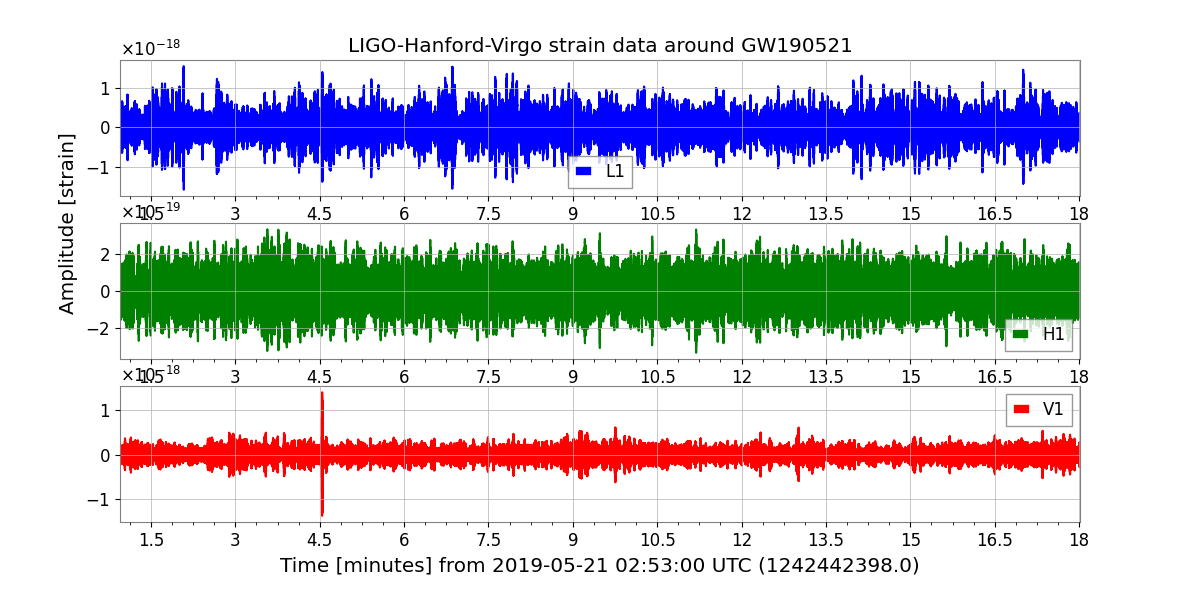
\includegraphics[width=0.6\textwidth]{GWanalysisProject_codefile/strainplot/GW190521strain.png}
            \caption{Strain data , with respect to time, recorded by each detector L1, H1 and V1 around GW190521}
            \label{fig:GW190521strain}
\end{figure}

\begin{figure}[htb]
    \centering
    \begin{subfigure}{0.45\textwidth}
       \centering
    
      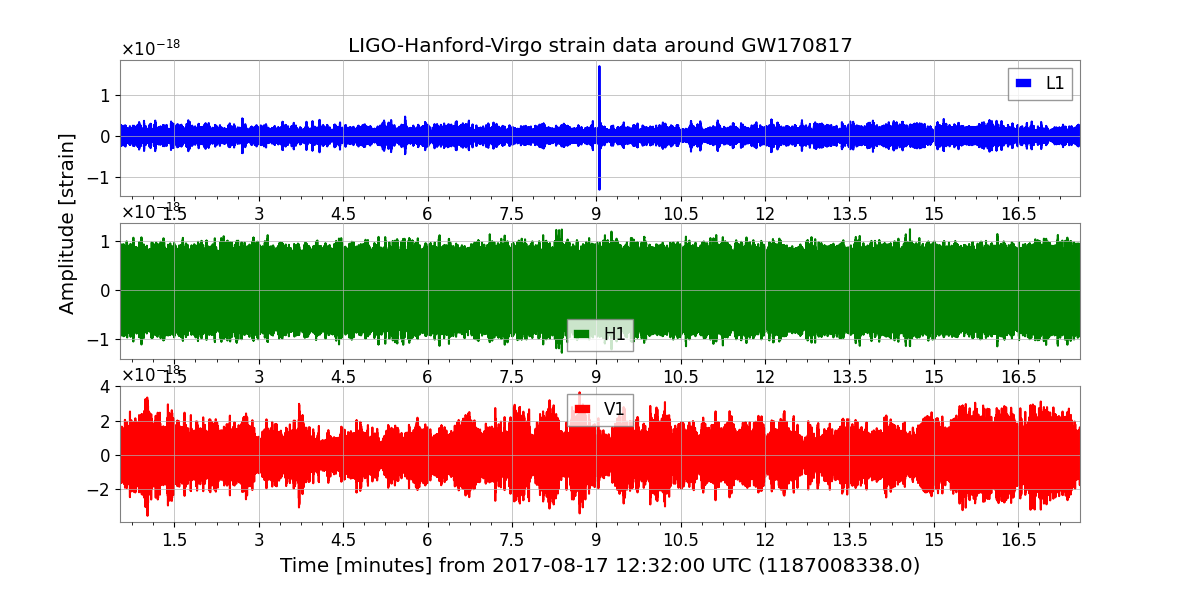
\includegraphics[width=1.27\linewidth]{GWanalysisProject_codefile/strainplot/GW170817strain.png}
           \caption{Strain data of GW170817}
           \label{fig: gw170817strain}
    \end{subfigure}
    % \hfill
    \begin{subfigure}{0.45\textwidth}
        \centering
        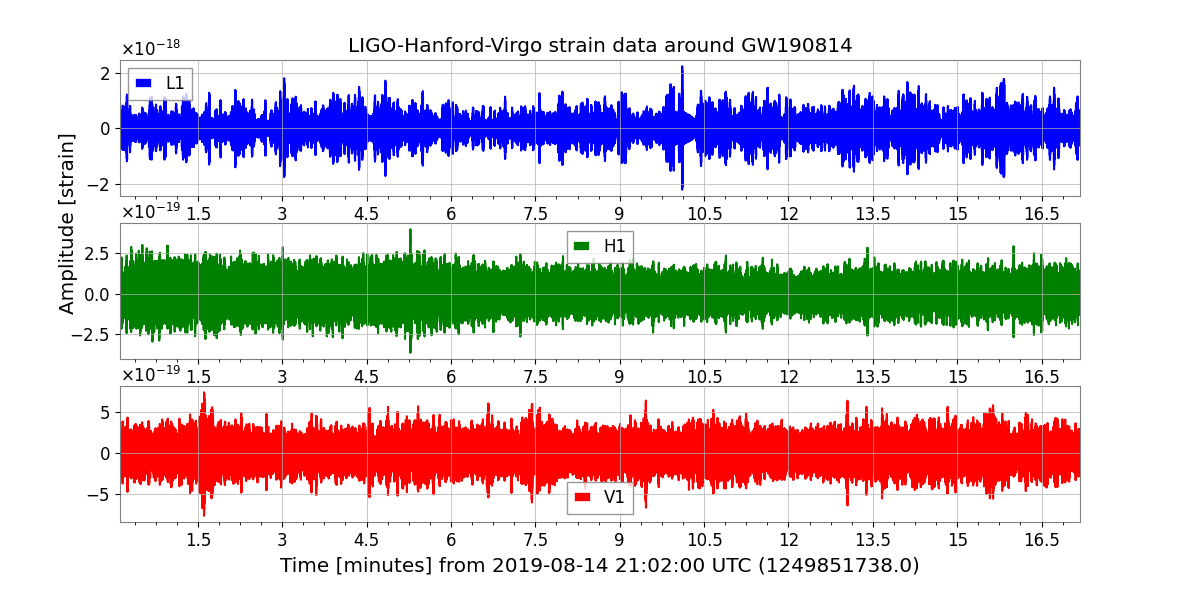
\includegraphics[width=1.27\linewidth]{GWanalysisProject_codefile/strainplot/GW190814strain.png}
        \caption{Strain data of GW190814}
        \label{fig: gw190521strain}
    \end{subfigure}
    \caption{Strain data , with respect to time, recorded by each detector L1, H1 and V1 around GW170817 and GW190814}
    \label{fig: strainplot}
\end{figure}

% start from here for description of asd plot
Important information on the noise properties of each instrument is provided by the Amplitude Spectral Density plot of the gravitational wave event, as observed by the LIGO-Livingston, LIGO-Hanford, and VIRGO detectors. 

\begin{figure}[htb]
    \centering
    \begin{subfigure}{0.45\textwidth}
       \centering
       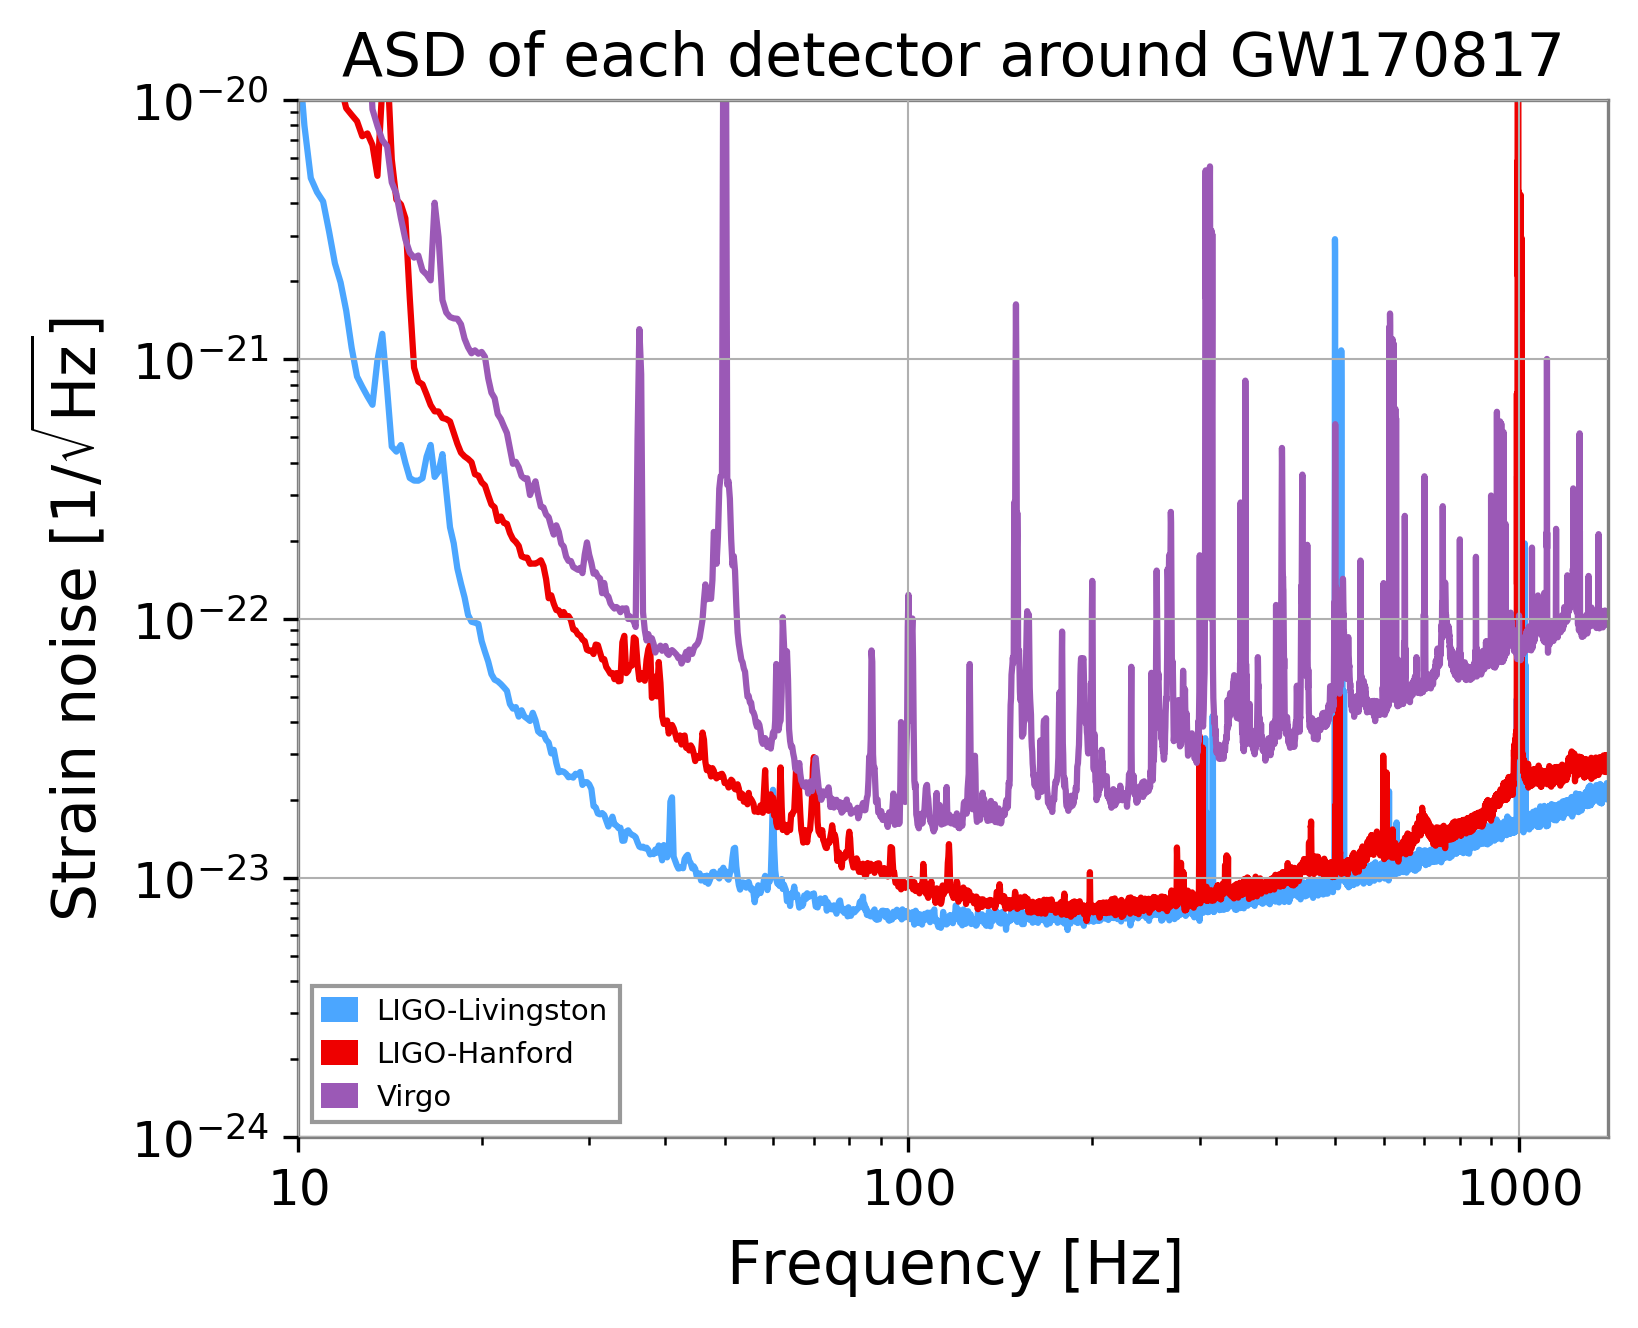
\includegraphics[width=1.0\linewidth]{GWanalysisProject_codefile/asd_plot/GW170817asd.png}
       \label{fig: gw170817asd}
    \end{subfigure}
    \hfill
    \begin{subfigure}{0.45\textwidth}
        \centering
        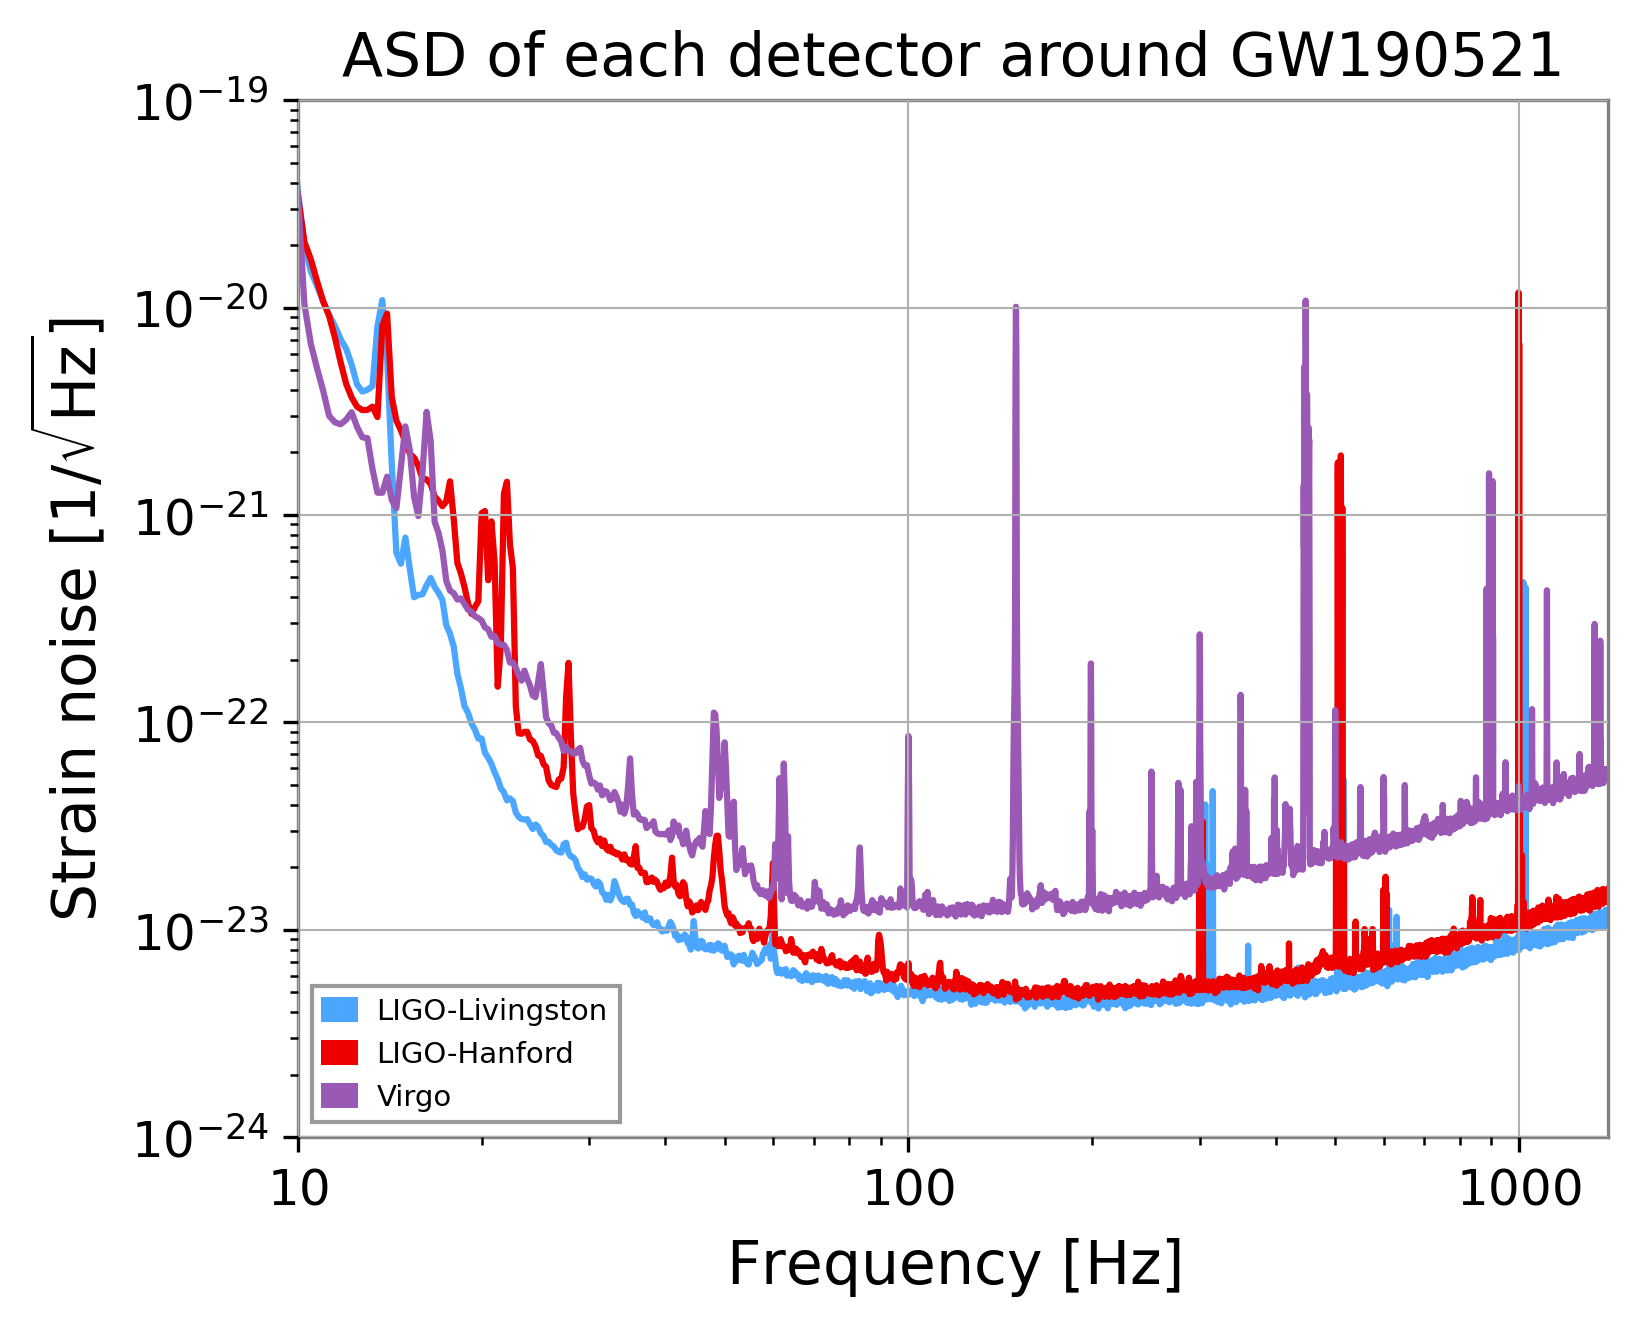
\includegraphics[width=1.0\linewidth]{GWanalysisProject_codefile/asd_plot/GW190521asd.png}
        \label{fig: gw190814asd}
    \end{subfigure}
    \hfill
    \begin{subfigure}{0.45\textwidth}
        \centering
        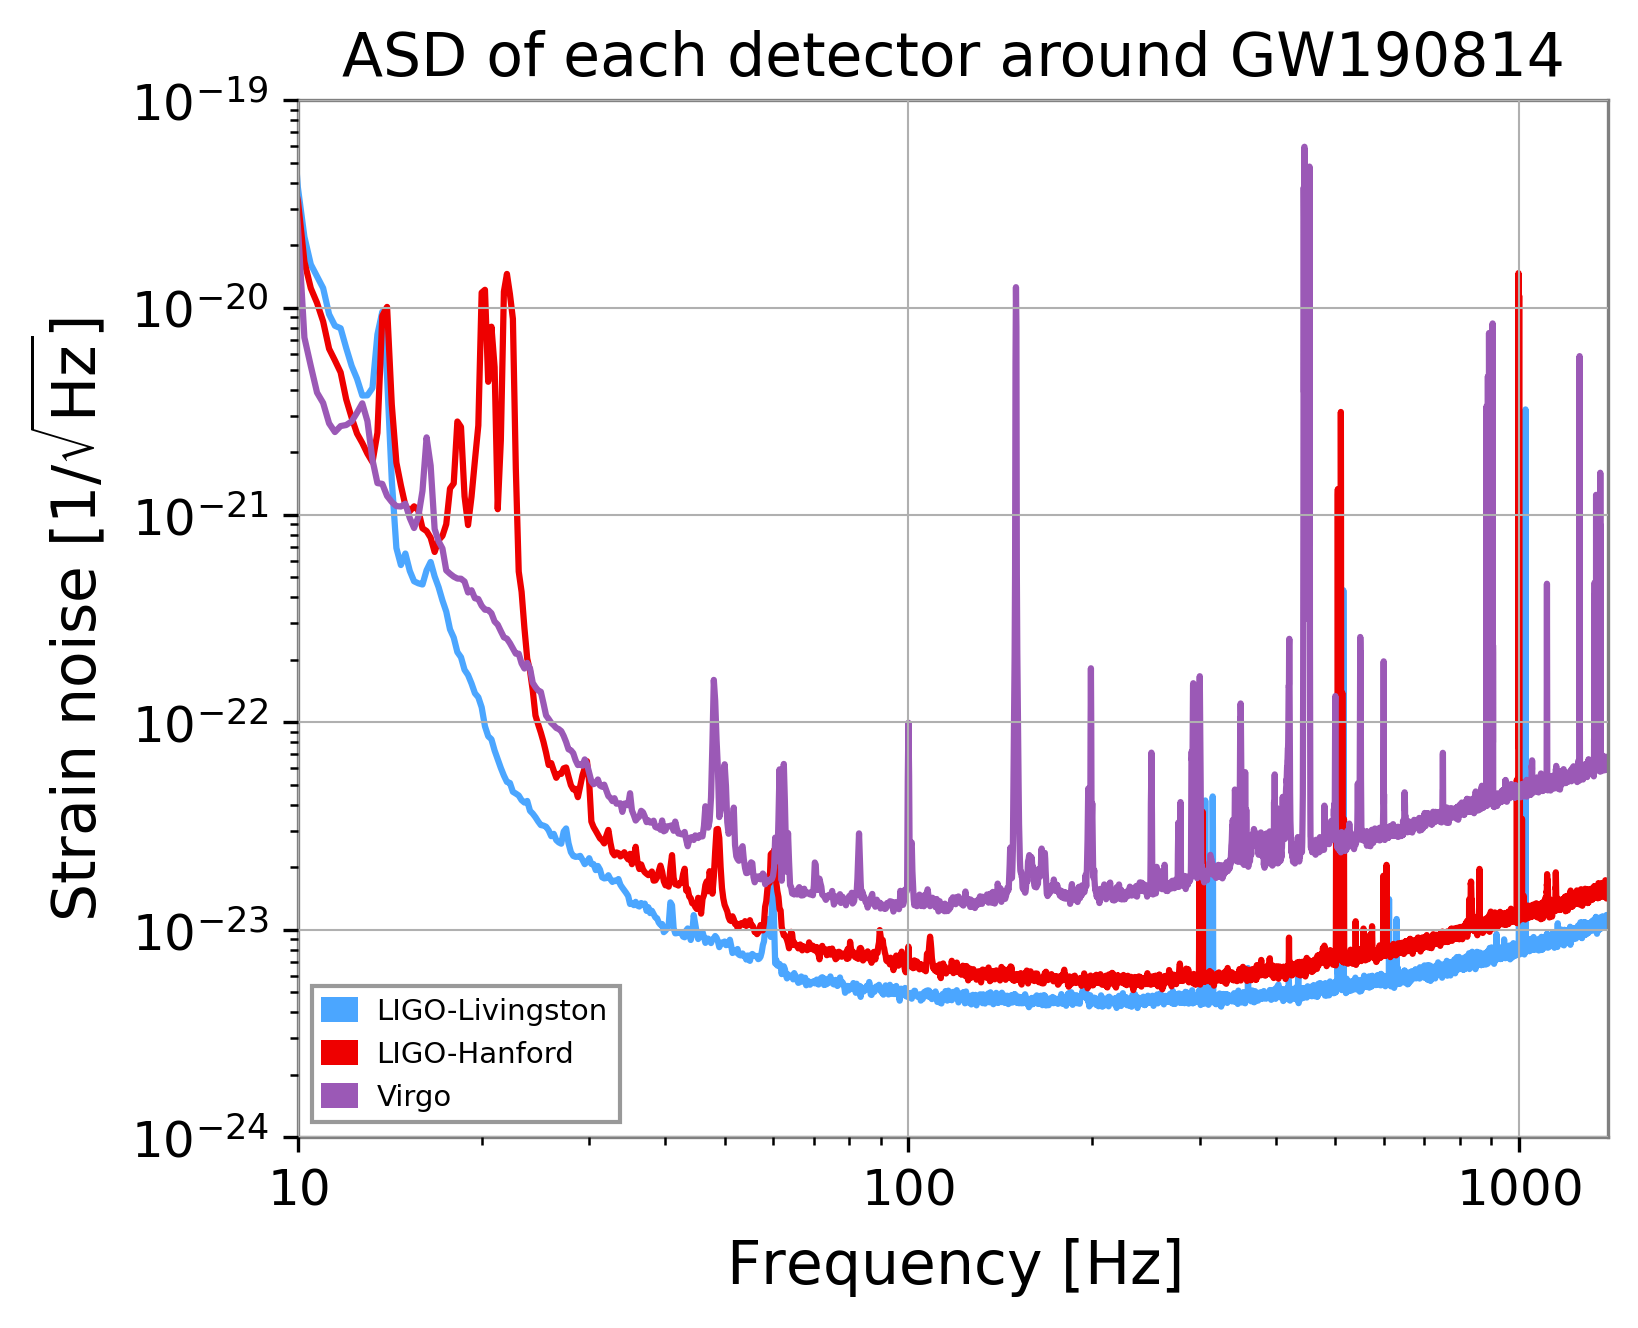
\includegraphics[width=1.0\linewidth]{GWanalysisProject_codefile/asd_plot/GW190814asd.png}
        \label{fig: gw190521asd}
    \end{subfigure}
    \caption{Amplitude Spectral Density (ASD) of each detector around GW170817, GW190521 and GW190814}
    \label{fig: asdplot}
\end{figure}

The Amplitude Spectral Density graphs of the LIGO and VIRGO detectors during the occurrences of GW170817, GW190814, and GW190521 offer significant insights into the detectors' sensitivity. In the case of GW170817, the LIGO-Livingston detector displayed the lowest strain noise over a wide range of frequencies, indicating superior sensitivity. The LIGO-Hanford detector, on the other hand, reported somewhat greater levels of noise. Above 100 Hz, the VIRGO detector exhibited the maximum level of strain noise, as seen by the purple curve. At lower frequencies (10-100 Hz), the level of strain noise reduced as the frequency increased, mostly because of the presence of seismic and ambient noise. At around 100 Hz, all detectors reached their maximum sensitivity with little strain noise, which subsequently rose at higher frequencies (100-1000 Hz) as a result of thermal and quantum noise.

Similarly, in the cases of the GW190814 and GW190521 events, the LIGO-Livingston detector consistently exhibited the highest sensitivity with the lowest level of strain noise. It was followed by the LIGO-Hanford detector, while the VIRGO detector had the highest level of strain noise. The VIRGO detector displayed many distinct peaks at various frequencies, suggesting the presence of narrowband noise sources or resonances. 


\begin{figure}[htb]
    \centering
    \begin{subfigure}{0.45\textwidth}
       \centering
       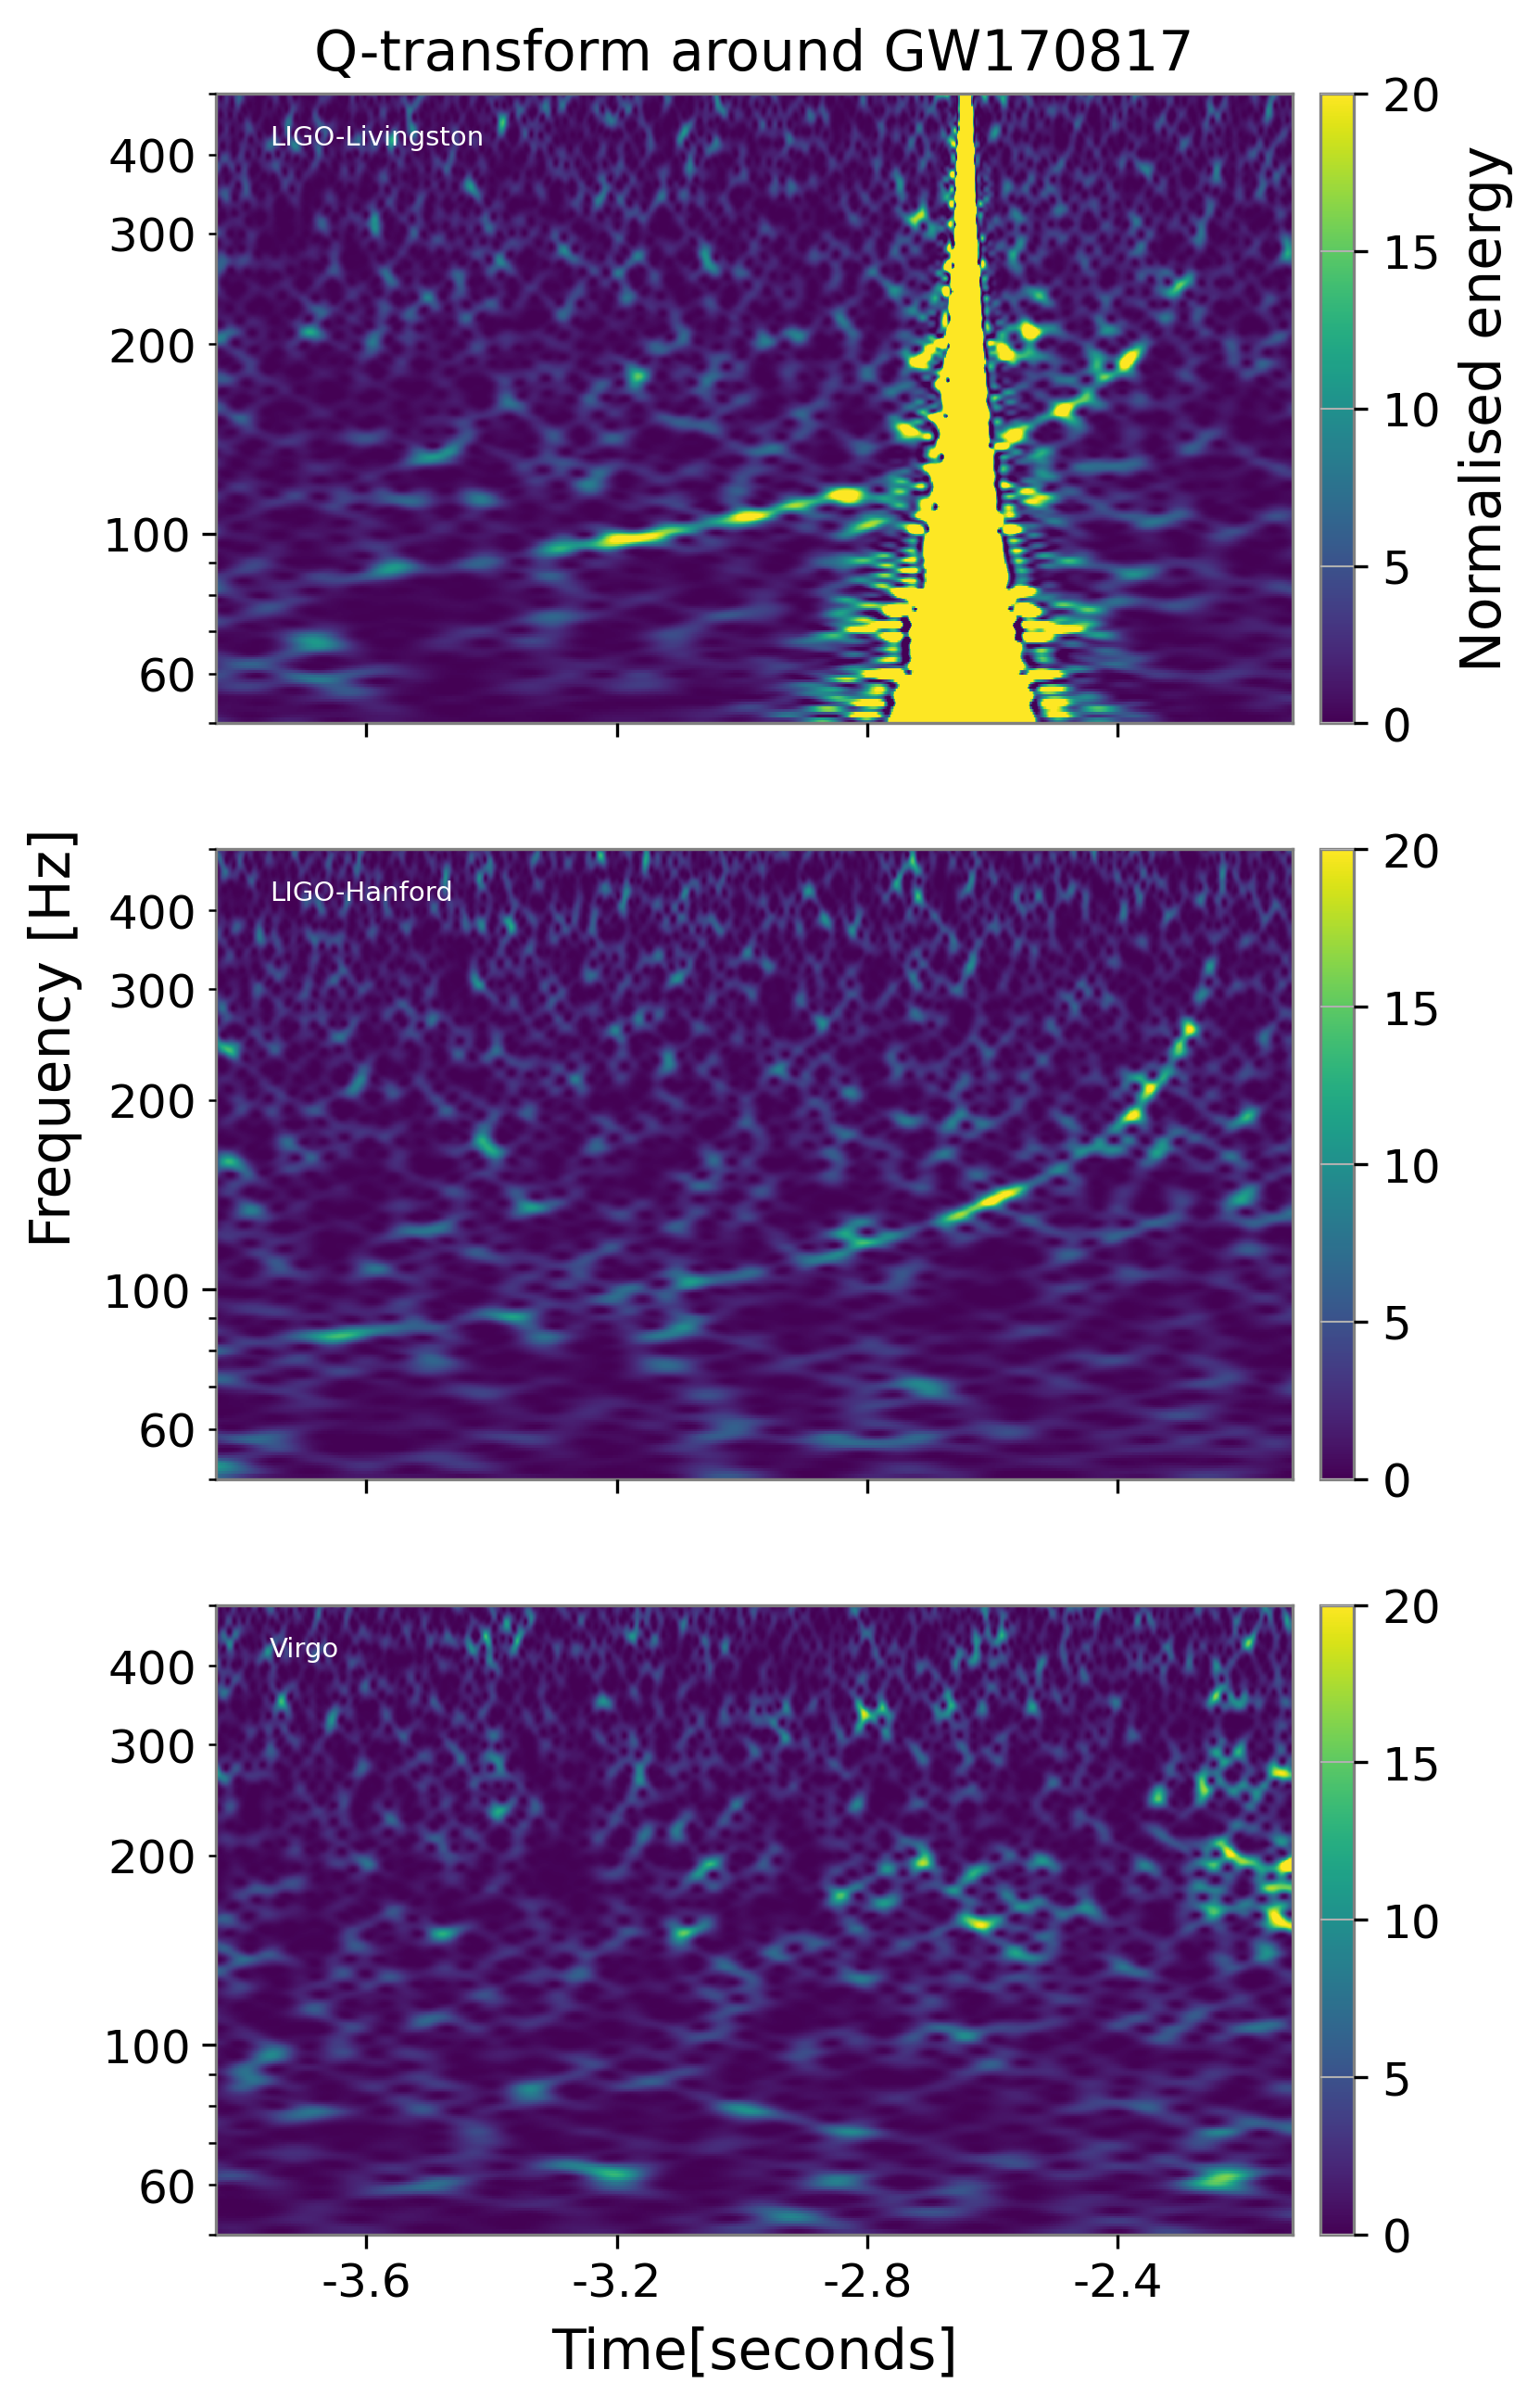
\includegraphics[width=0.65\linewidth]{GWanalysisProject_codefile/qtransformplot/GW170817_qtransform.png}
       \label{fig: gw170817qtransform}
    \end{subfigure}
    \hfill
    \begin{subfigure}{0.45\textwidth}
        \centering
        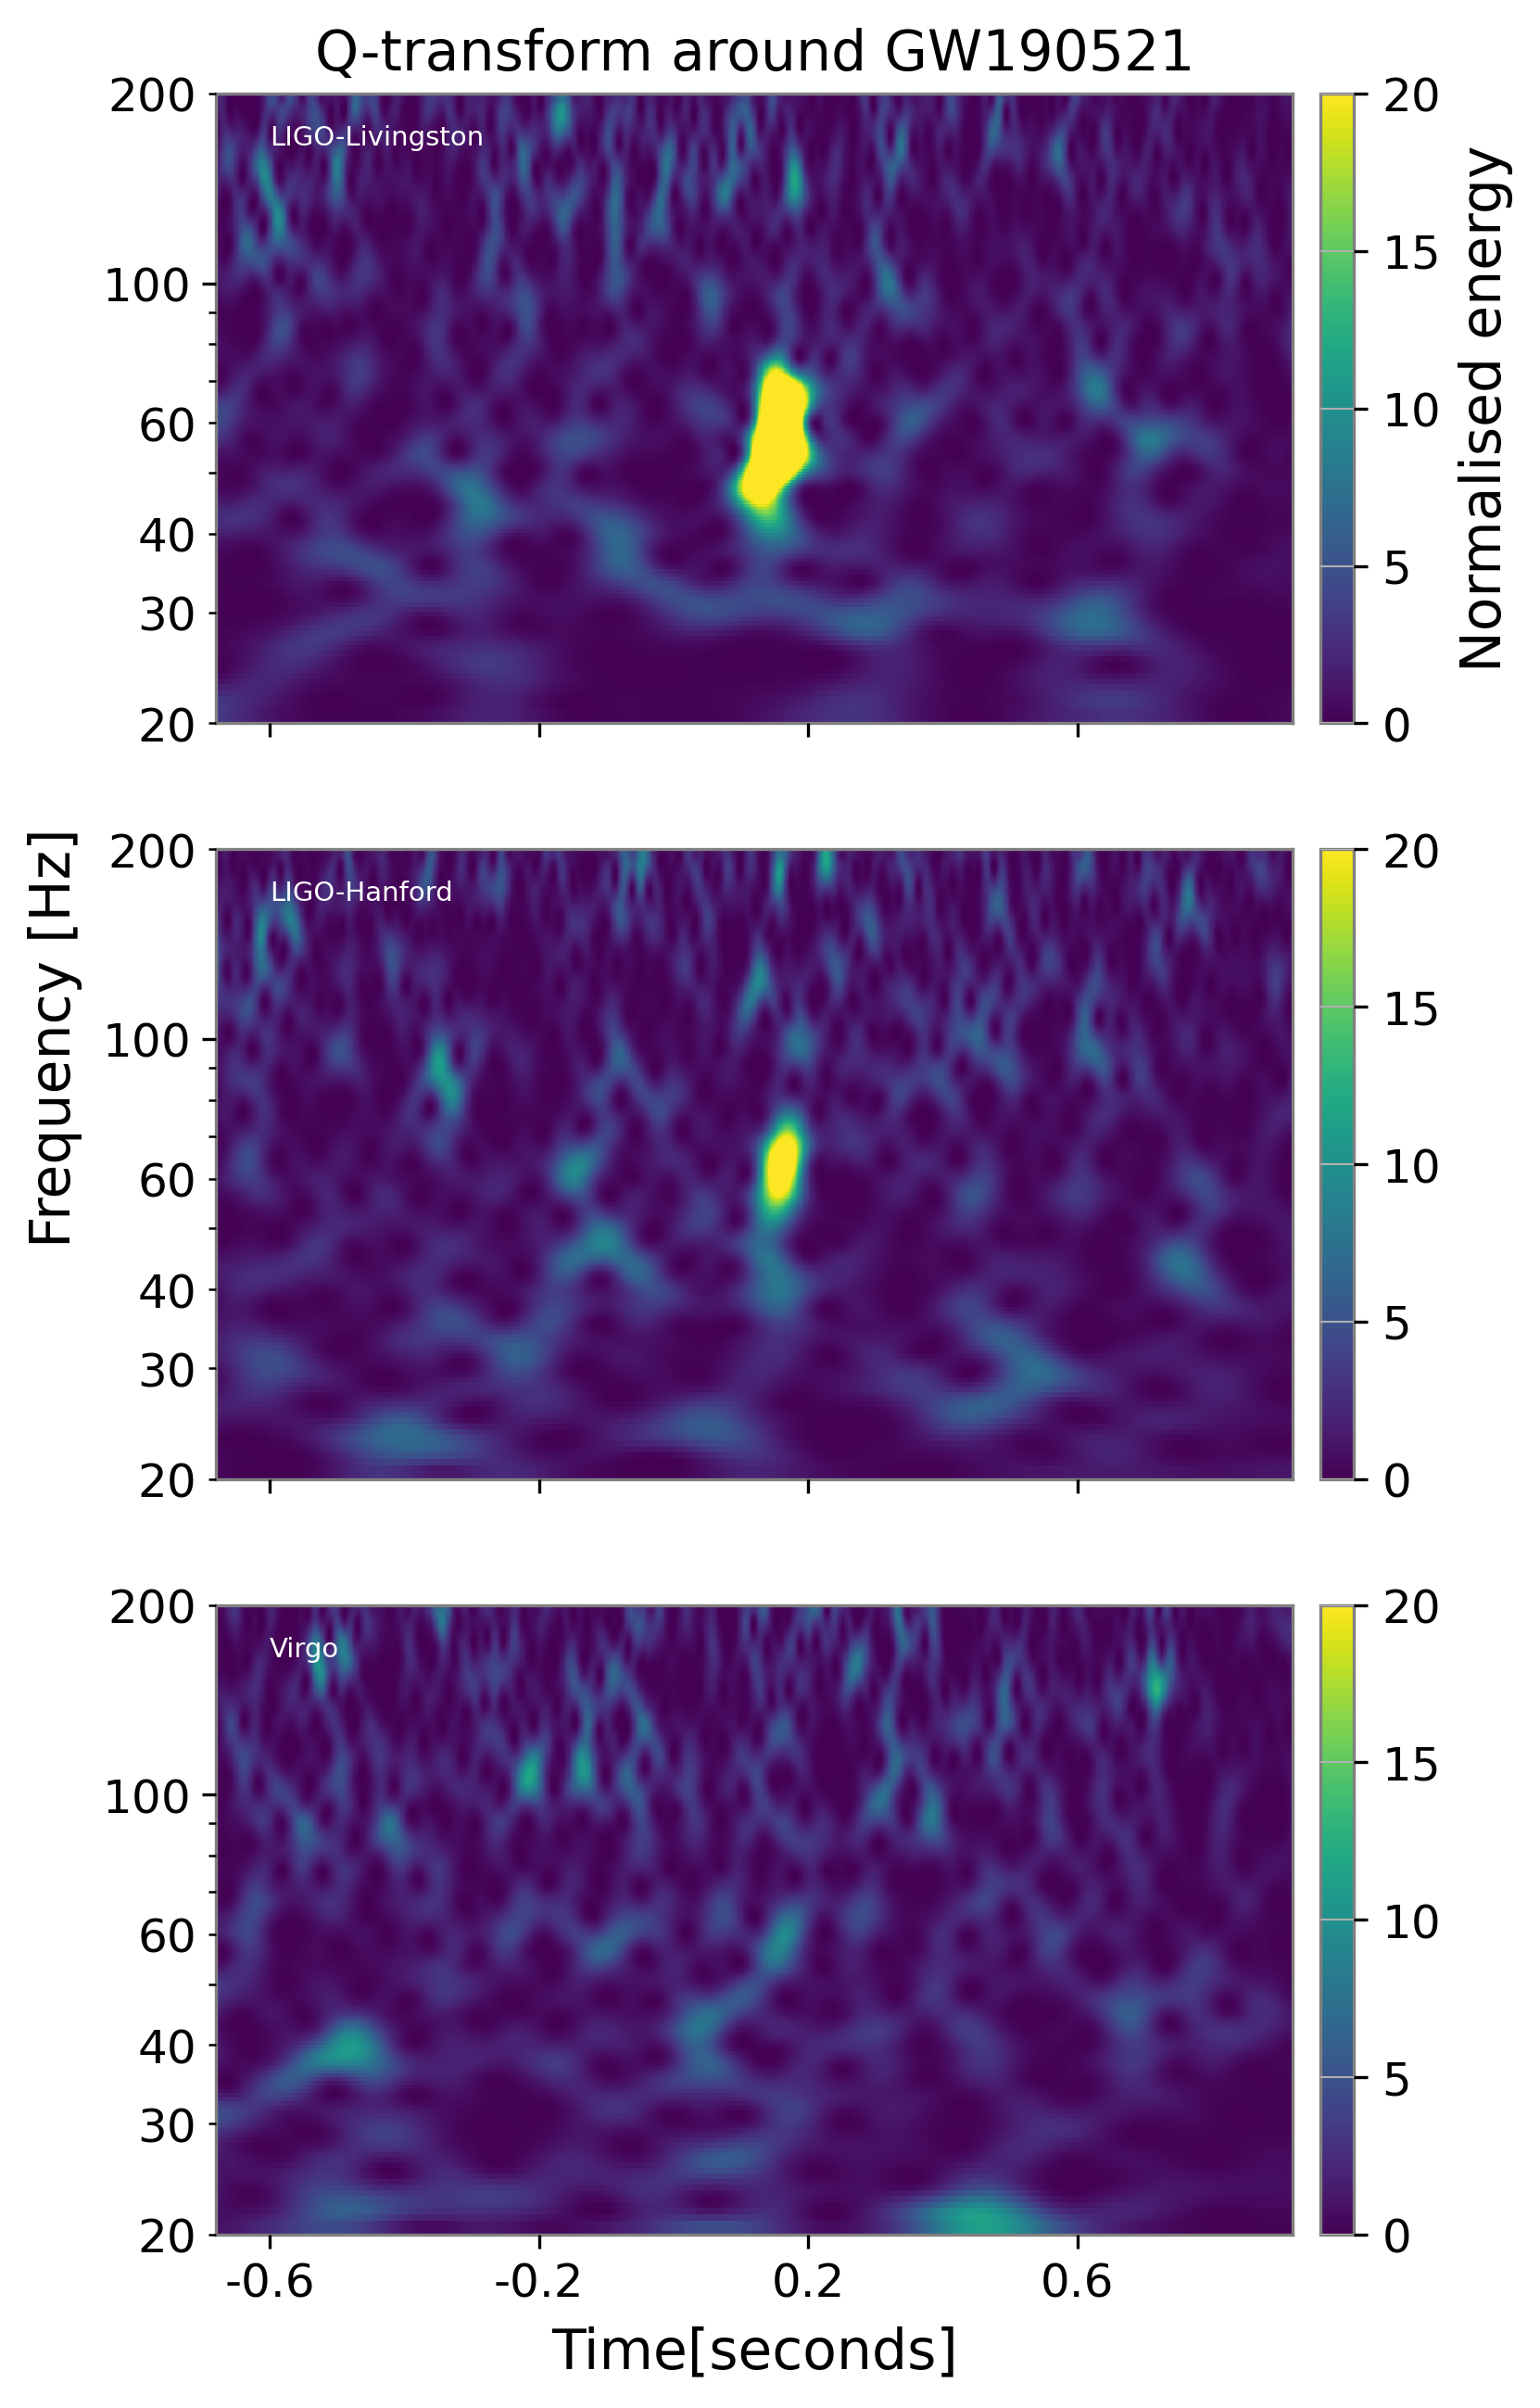
\includegraphics[width=0.65\linewidth]{GWanalysisProject_codefile/qtransformplot/GW190521_qtransform.png}
        \label{fig: gw190814qtransform}
    \end{subfigure}
    \hfill
    \begin{subfigure}{0.45\textwidth}
        \centering
        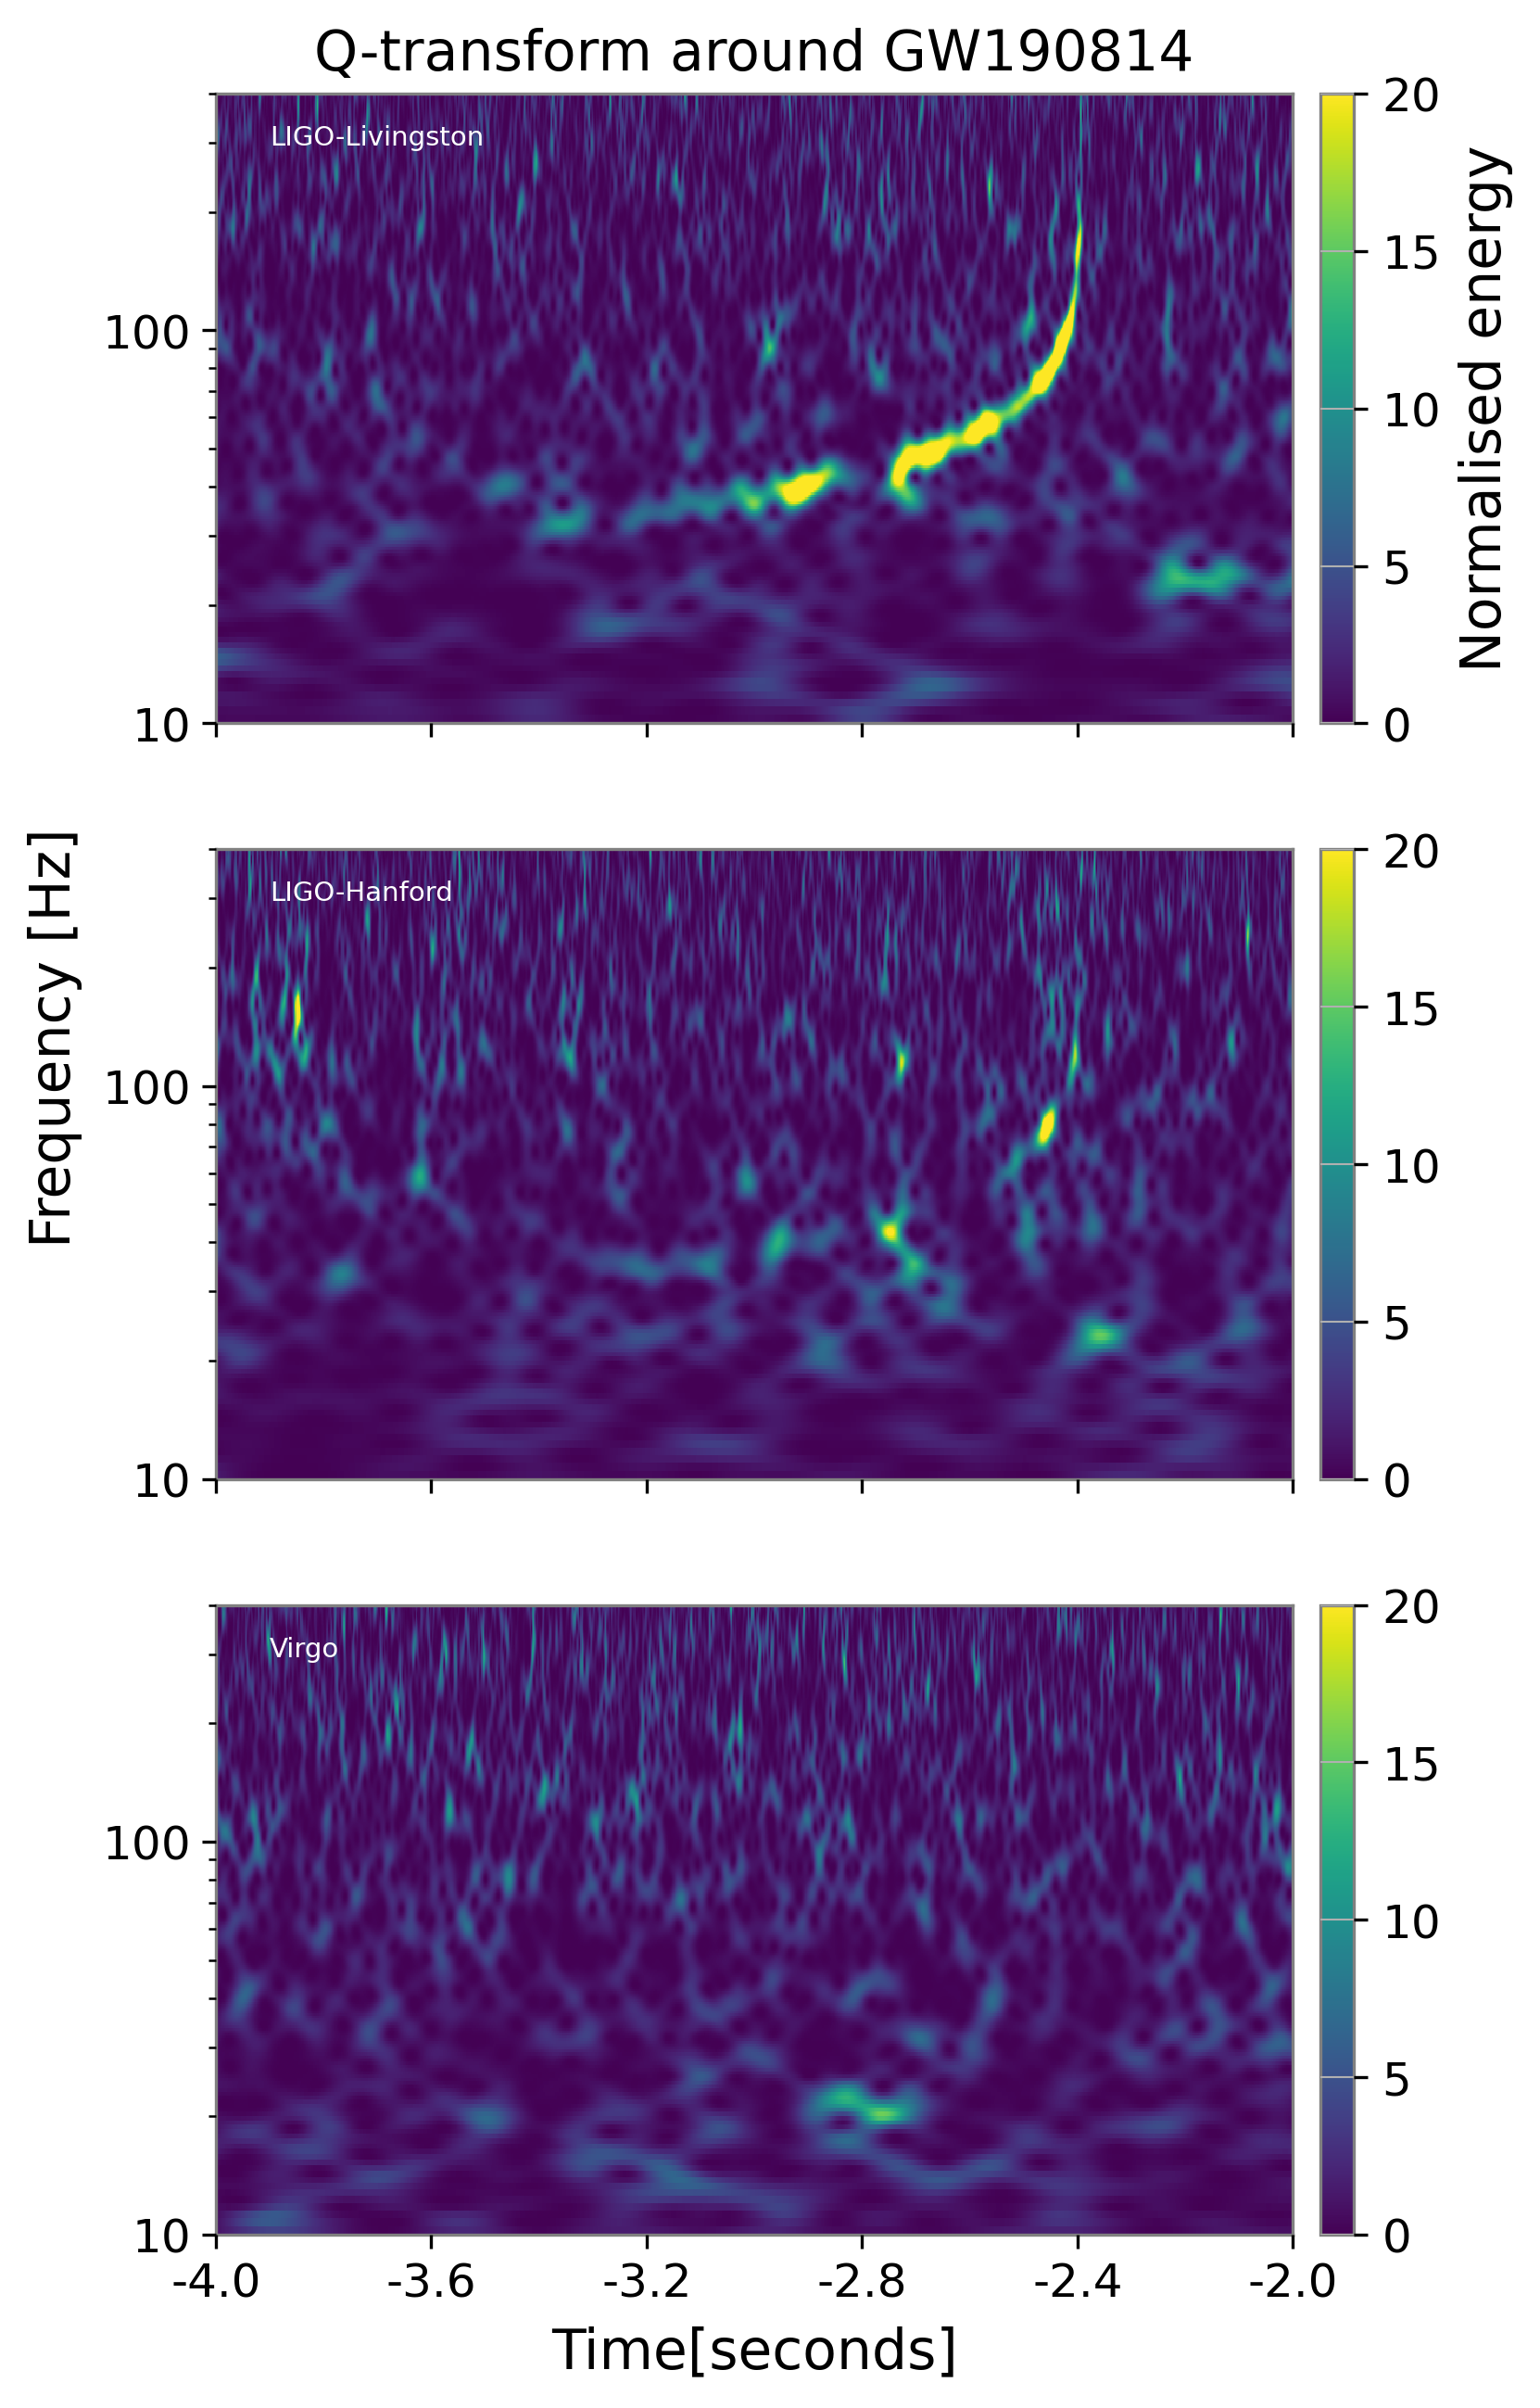
\includegraphics[width=0.65\linewidth]{GWanalysisProject_codefile/qtransformplot/GW190814_qtransform.png}
        \label{fig: gw190521qtransform}
    \end{subfigure}
    \caption{Amplitude Spectral Density of each detector around GW170817, GW190521 and GW190814}
    \label{fig: qtransformplot}
\end{figure}

Figure [\ref{fig: qtransformplot}] depicted a two-dimensional spectrogram of the data, illustrating the variations in strength of the gravity waves at different frequencies during the event. 
The spectrograms of GW170817 exhibit a distinct chirp signal, with the most notable instance detected in the LIGO-Livingston data. The chirp signal may be observed as a vivid yellow streak, starting at a frequency of around 60 Hz and quickly rising to over 300 Hz as the event moves closer to the merger. The increase in both the frequency and amplitude of the signal corresponds to the last phase of the binary neutron stars' approach towards each other, ultimately resulting in their merger. However, the LIGO-Livingston spectrogram exhibits a loud glitch occurring during the time frame of -2.8 to -2.1 seconds. Nevertheless, the chirp signal of GW170817 remains apparent. A comparable chirp is observed in the LIGO-Hanford spectrogram. On the other hand, the VIRGO spectrogram shows diminished prominent characteristics. 

Similarly, The GW190521 event exhibits a concise, low-frequency signal, predominantly centered around 60 Hz, as detected by the LIGO-Livingston and LIGO-Hanford detectors. This signal is most likely caused by the substantial mass of the colliding black holes. This brief transient signal, lasting for only a fraction of a second just before the merging of two objects, emphasizes the swift and immediate process of the merger. The VIRGO detector detected a signal of lesser magnitude, in line with its reduced sensitivity.

Similarly, the GW190814 event exhibits a unique chirp signal, which is particularly evident in the LIGO-Livingston data. The signal begins at a low frequency and swiftly rises as the two objects spiral inward and combine, exhibiting the typical behavior of a black hole and a compact object coalescence. The Hanford and VIRGO detector captures a less intense signal.

\begin{figure}[h]
            \centering          
            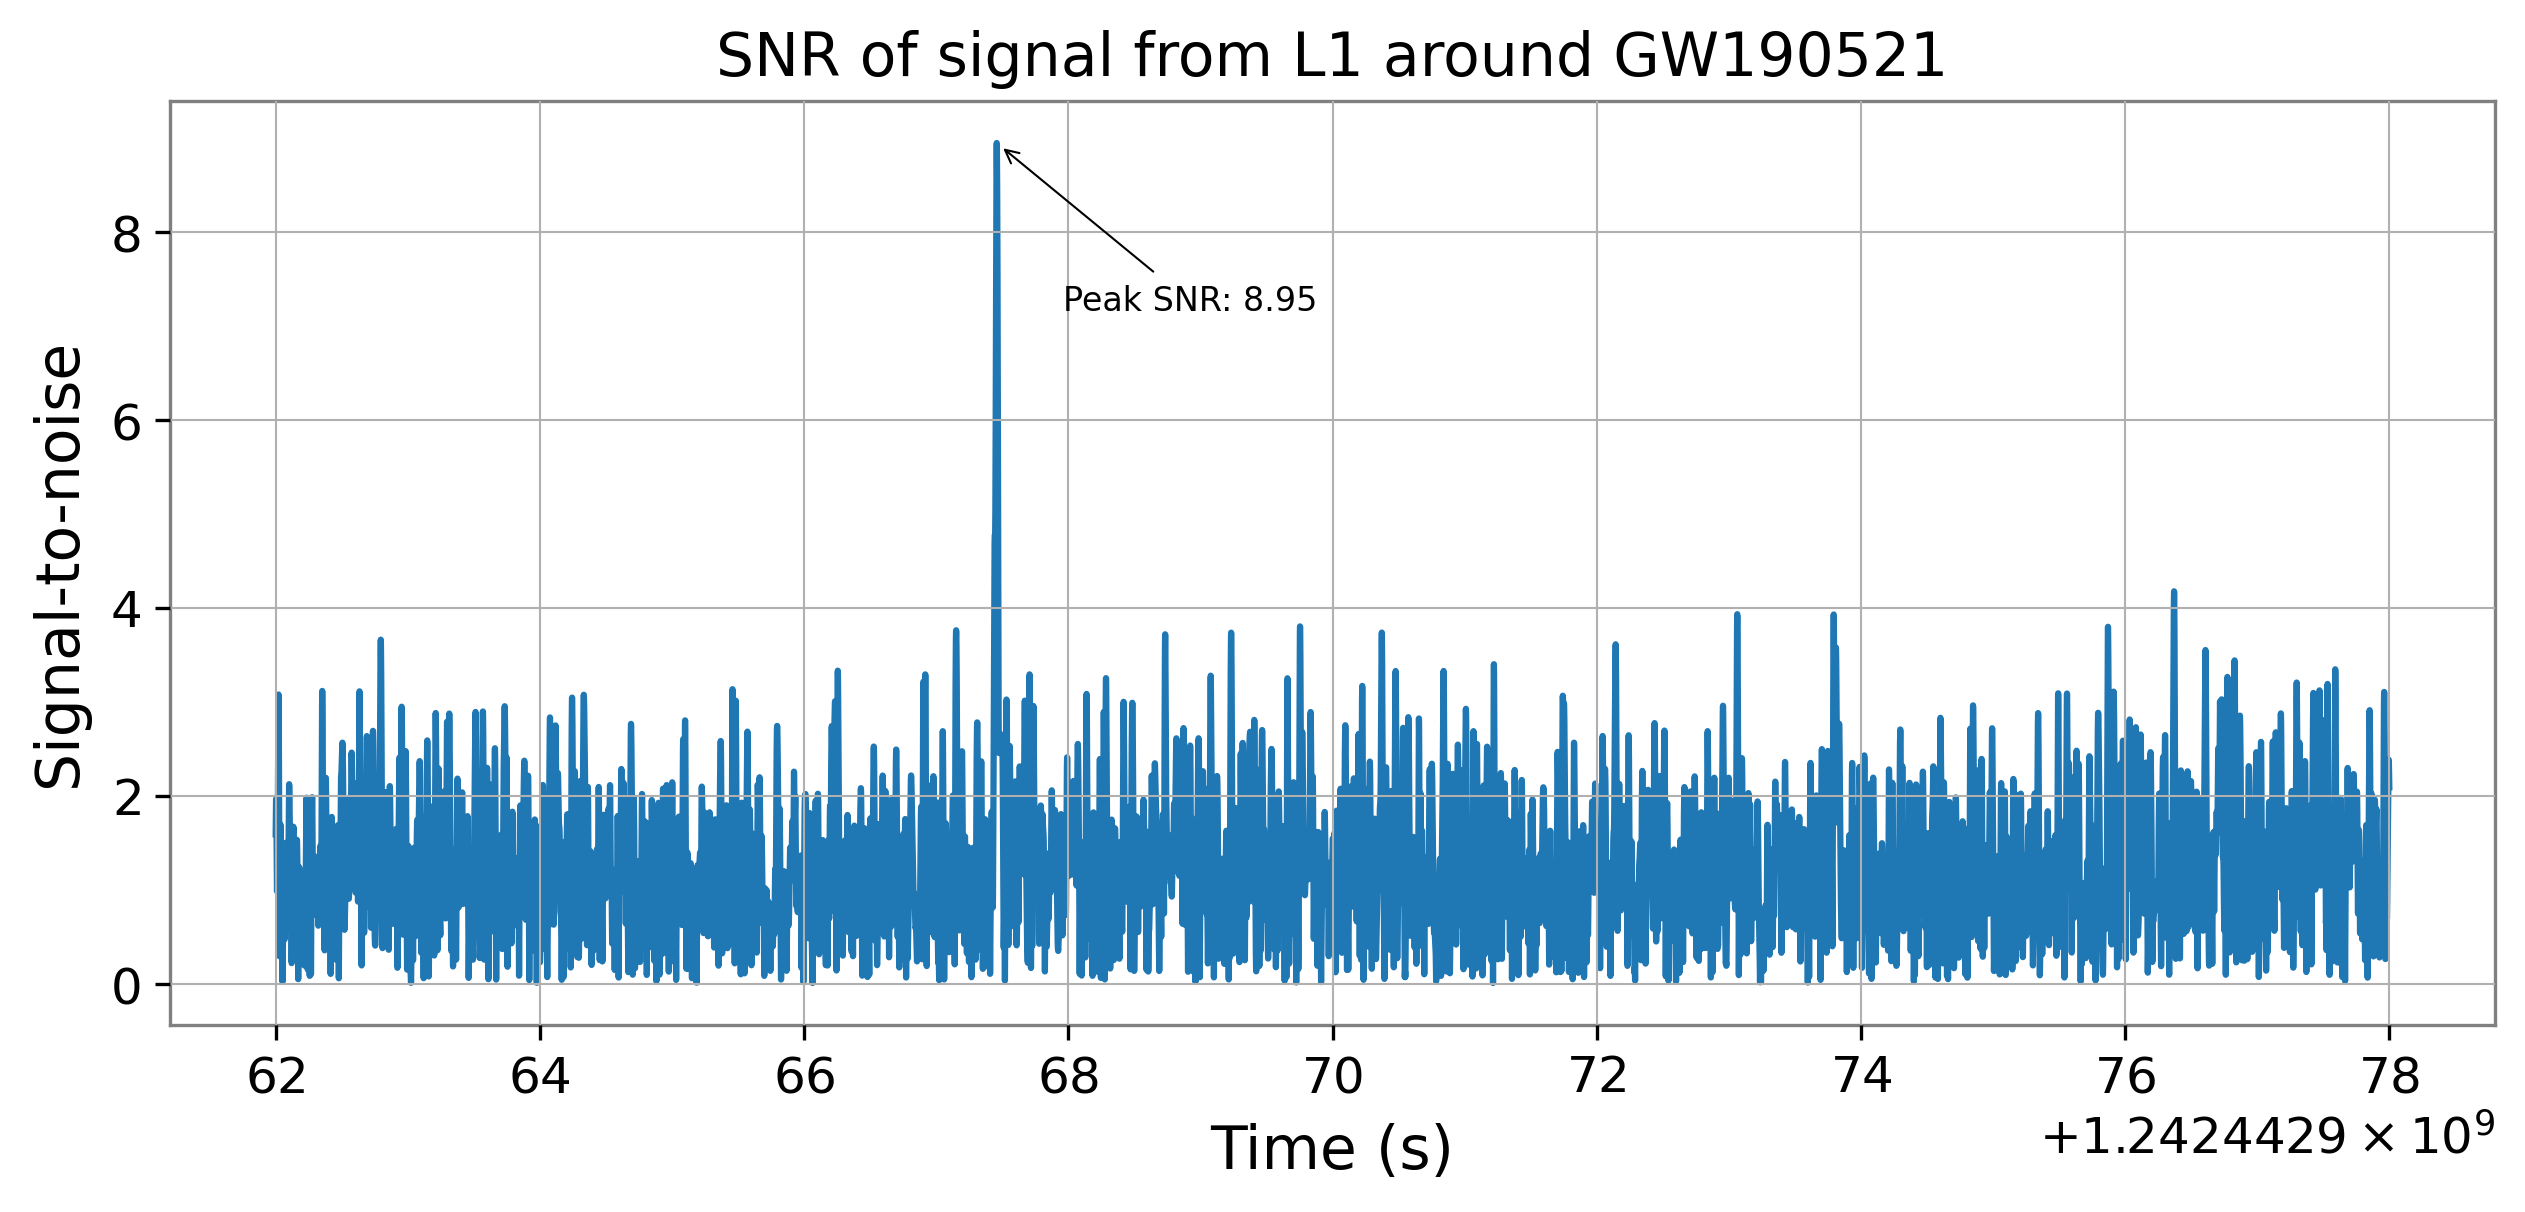
\includegraphics[width=0.85\textwidth]{GWanalysisProject_codefile/SNRplot/SNRL1GW190521.png}
            \caption{Signal to Noise Ratio around GW190521}
            \label{fig:GW190521SNR}
\end{figure}

\begin{figure}[h]
            \centering          
            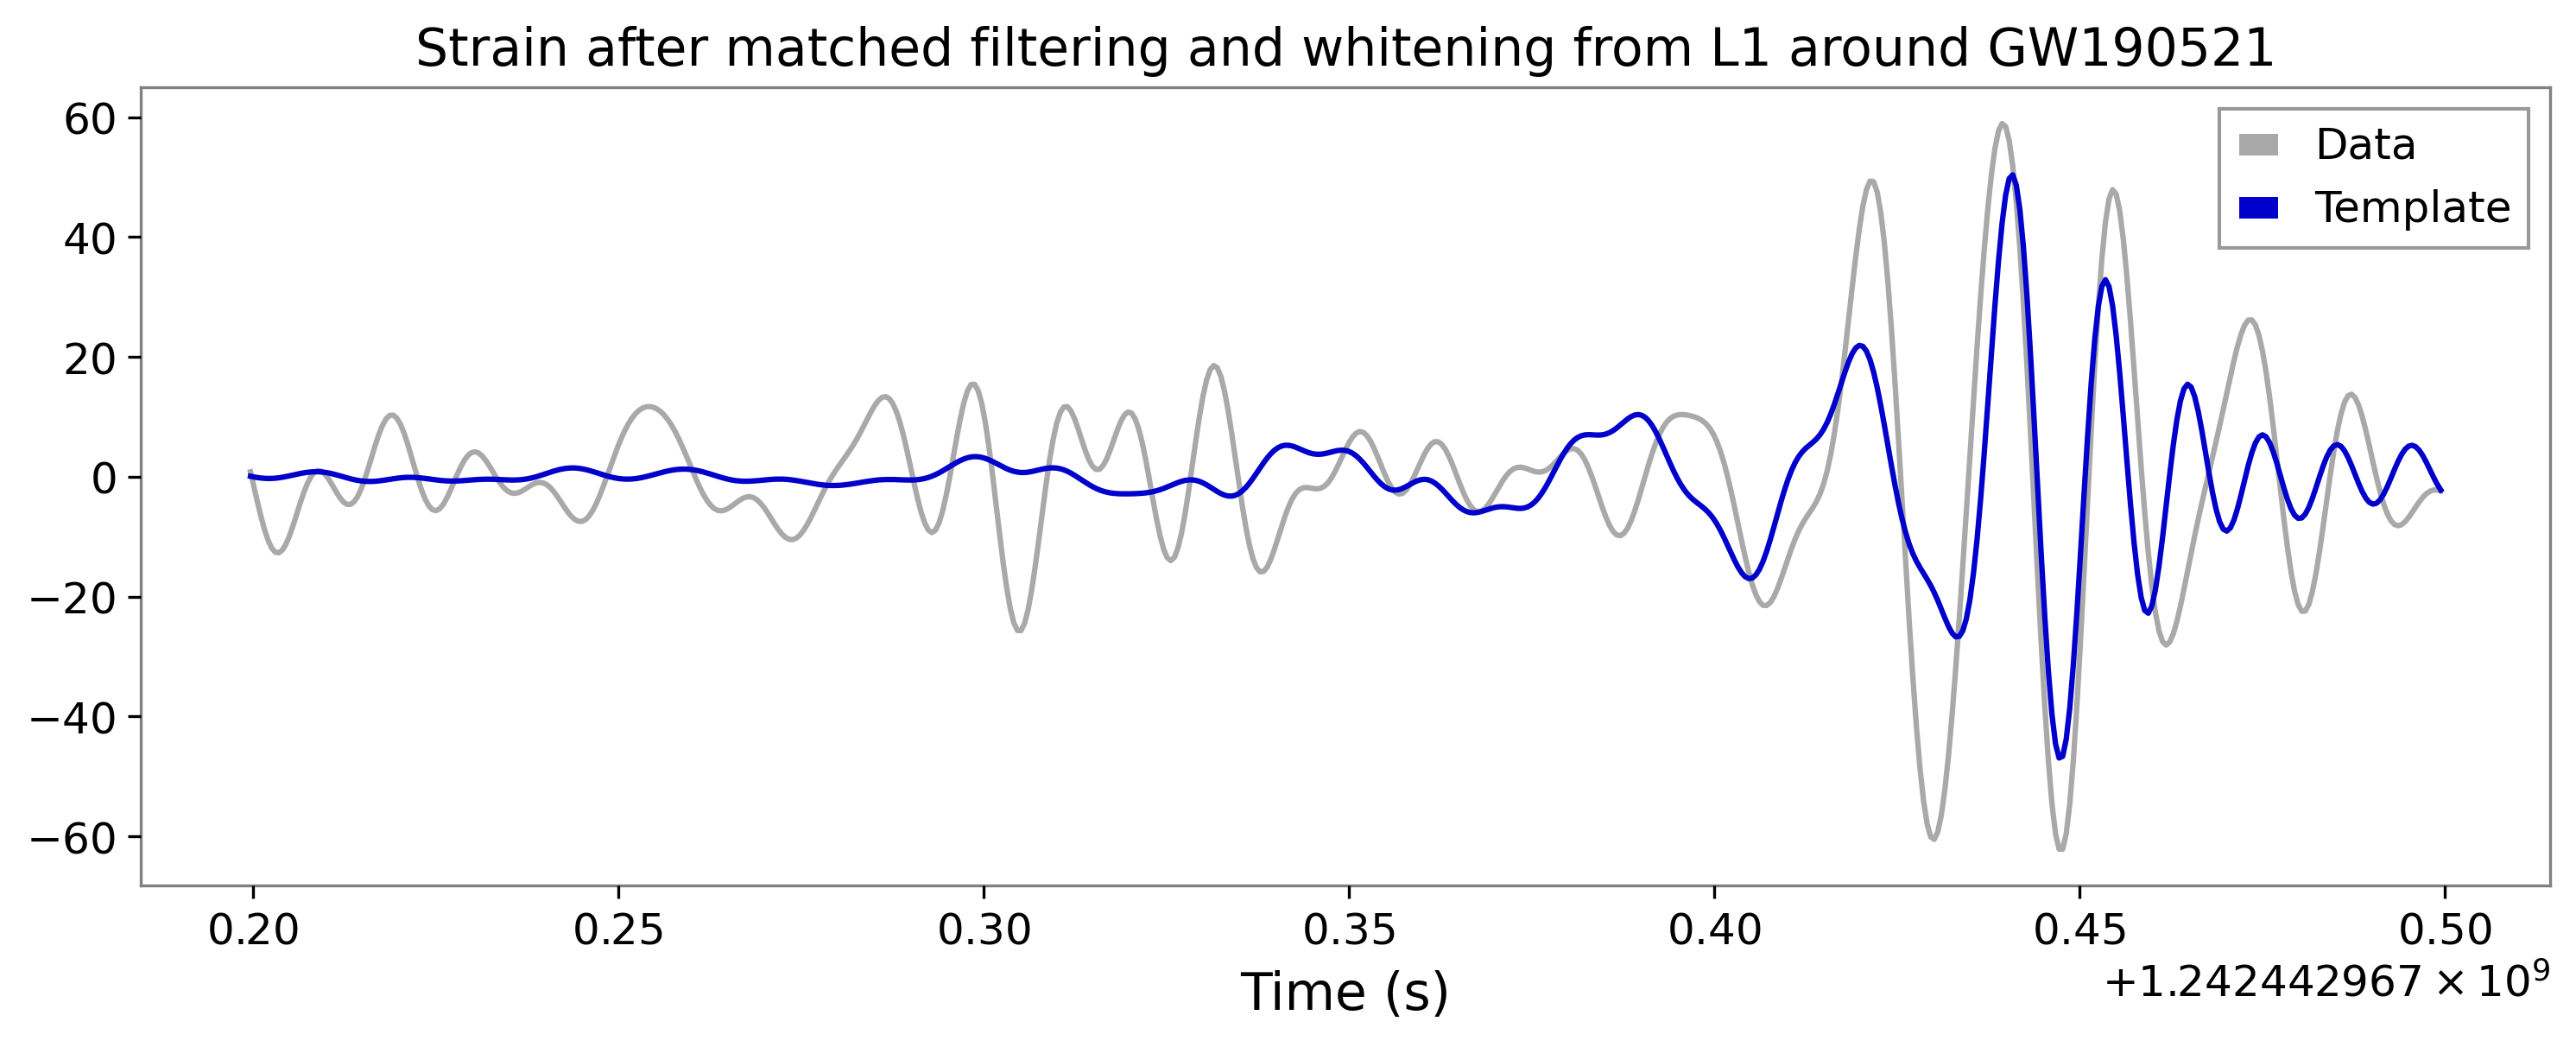
\includegraphics[width=0.85\textwidth]{GWanalysisProject_codefile/templateplot/templateL1GW190521.png}
            \caption{Whitened Template data calculated from numerical solution of GR and actual recorded data around GW190521}
            \label{fig:GW190521template}
\end{figure}


The Signal-to-Noise Ratio analysis was conducted on data from the L1 detector to identify the presence of a gravitational wave signal associated with the event GW190521. The signal-to-noise ratio measures the signal's intensity compared to the background noise, serving as a tool to evaluate the probability of a true gravitational wave signal being present in the observed data.

The SNR is graphed against time in figure \ref{fig:GW190521SNR}, with the time axis centered on the anticipated event time. The analysis showed a significant peak in the signal-to-noise ratio of 8.95 at around 68 seconds. The amplitude of this peak is considerably greater than the background noise, suggesting a robust detection of the signal.

% \begin{figure}[h]
%             \centering          
%             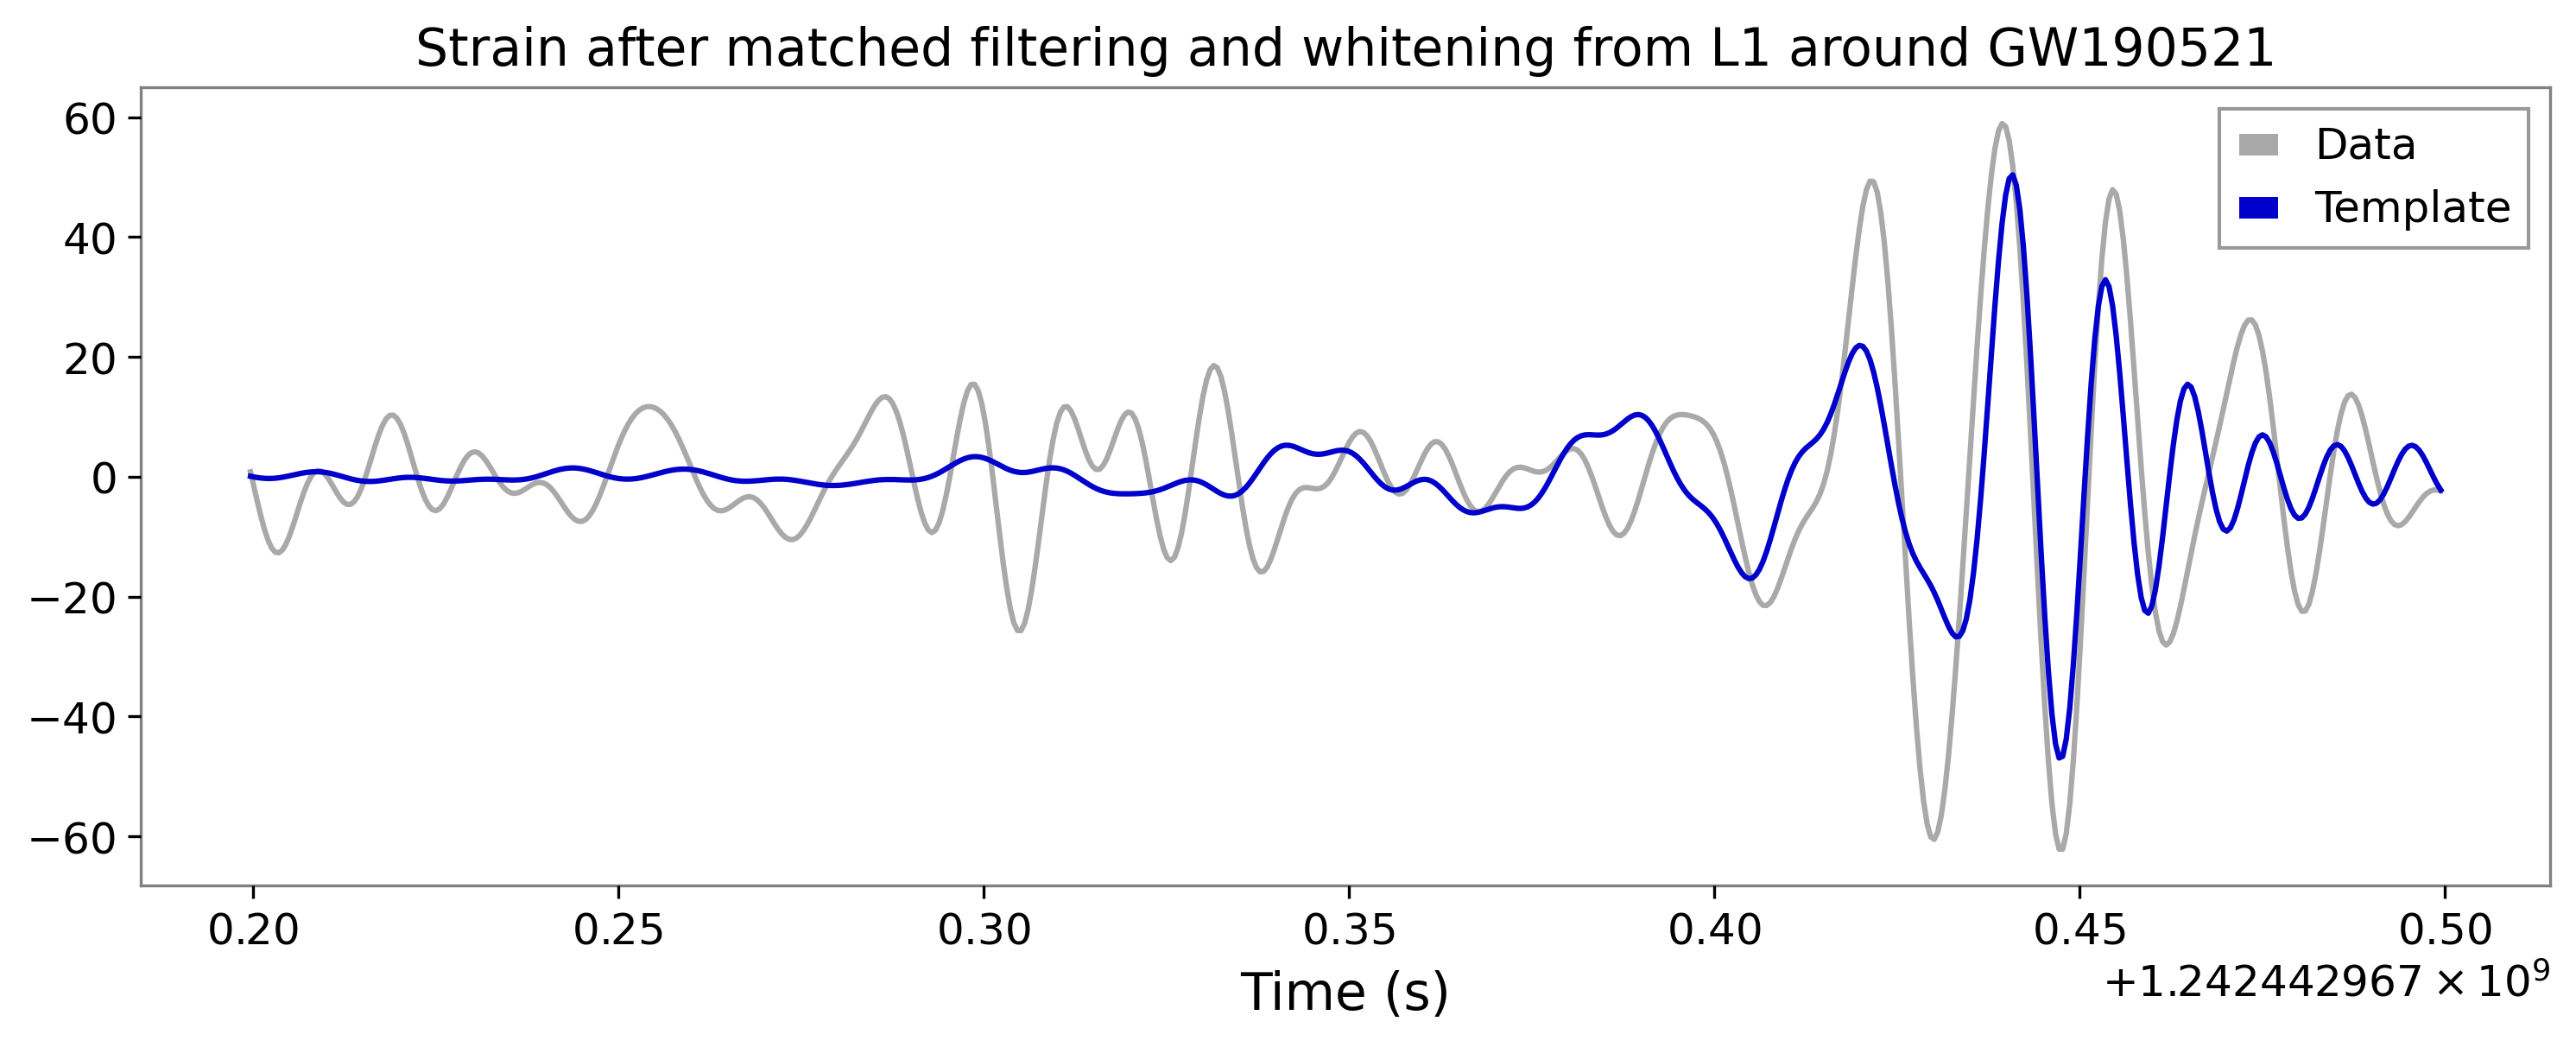
\includegraphics[width=0.95\textwidth]{GWanalysisProject_codefile/templateplot/templateL1GW190521.png}
%             \caption{Whitened Template data calculated from numerical solution of GR and actual recorded data around GW190521}
%             \label{fig:GW190521template}
% \end{figure}

We then generated a template plot by employing \texttt{get\_td\_waveform} function from the \texttt{pycbc.wa\\veform} module. Specifically, I used the waveform \texttt{approximant = 'IMRPhenomPv3HM'} (see Appendix \ref{code2}) with mass parameters of 90 and 65 $M_\odot$, and a distance of 4600 Mpc. The \texttt{'IMRPhen\\omPv3HM'} performs numerical solution of relativity of provided parameters. The waveform was computed with a time resolution of \texttt{conditioned.delta\_t} (see Appendix \ref{code2}) and a frequency lower bound of 20 Hz.
\begin{figure}[h]
            \centering          
            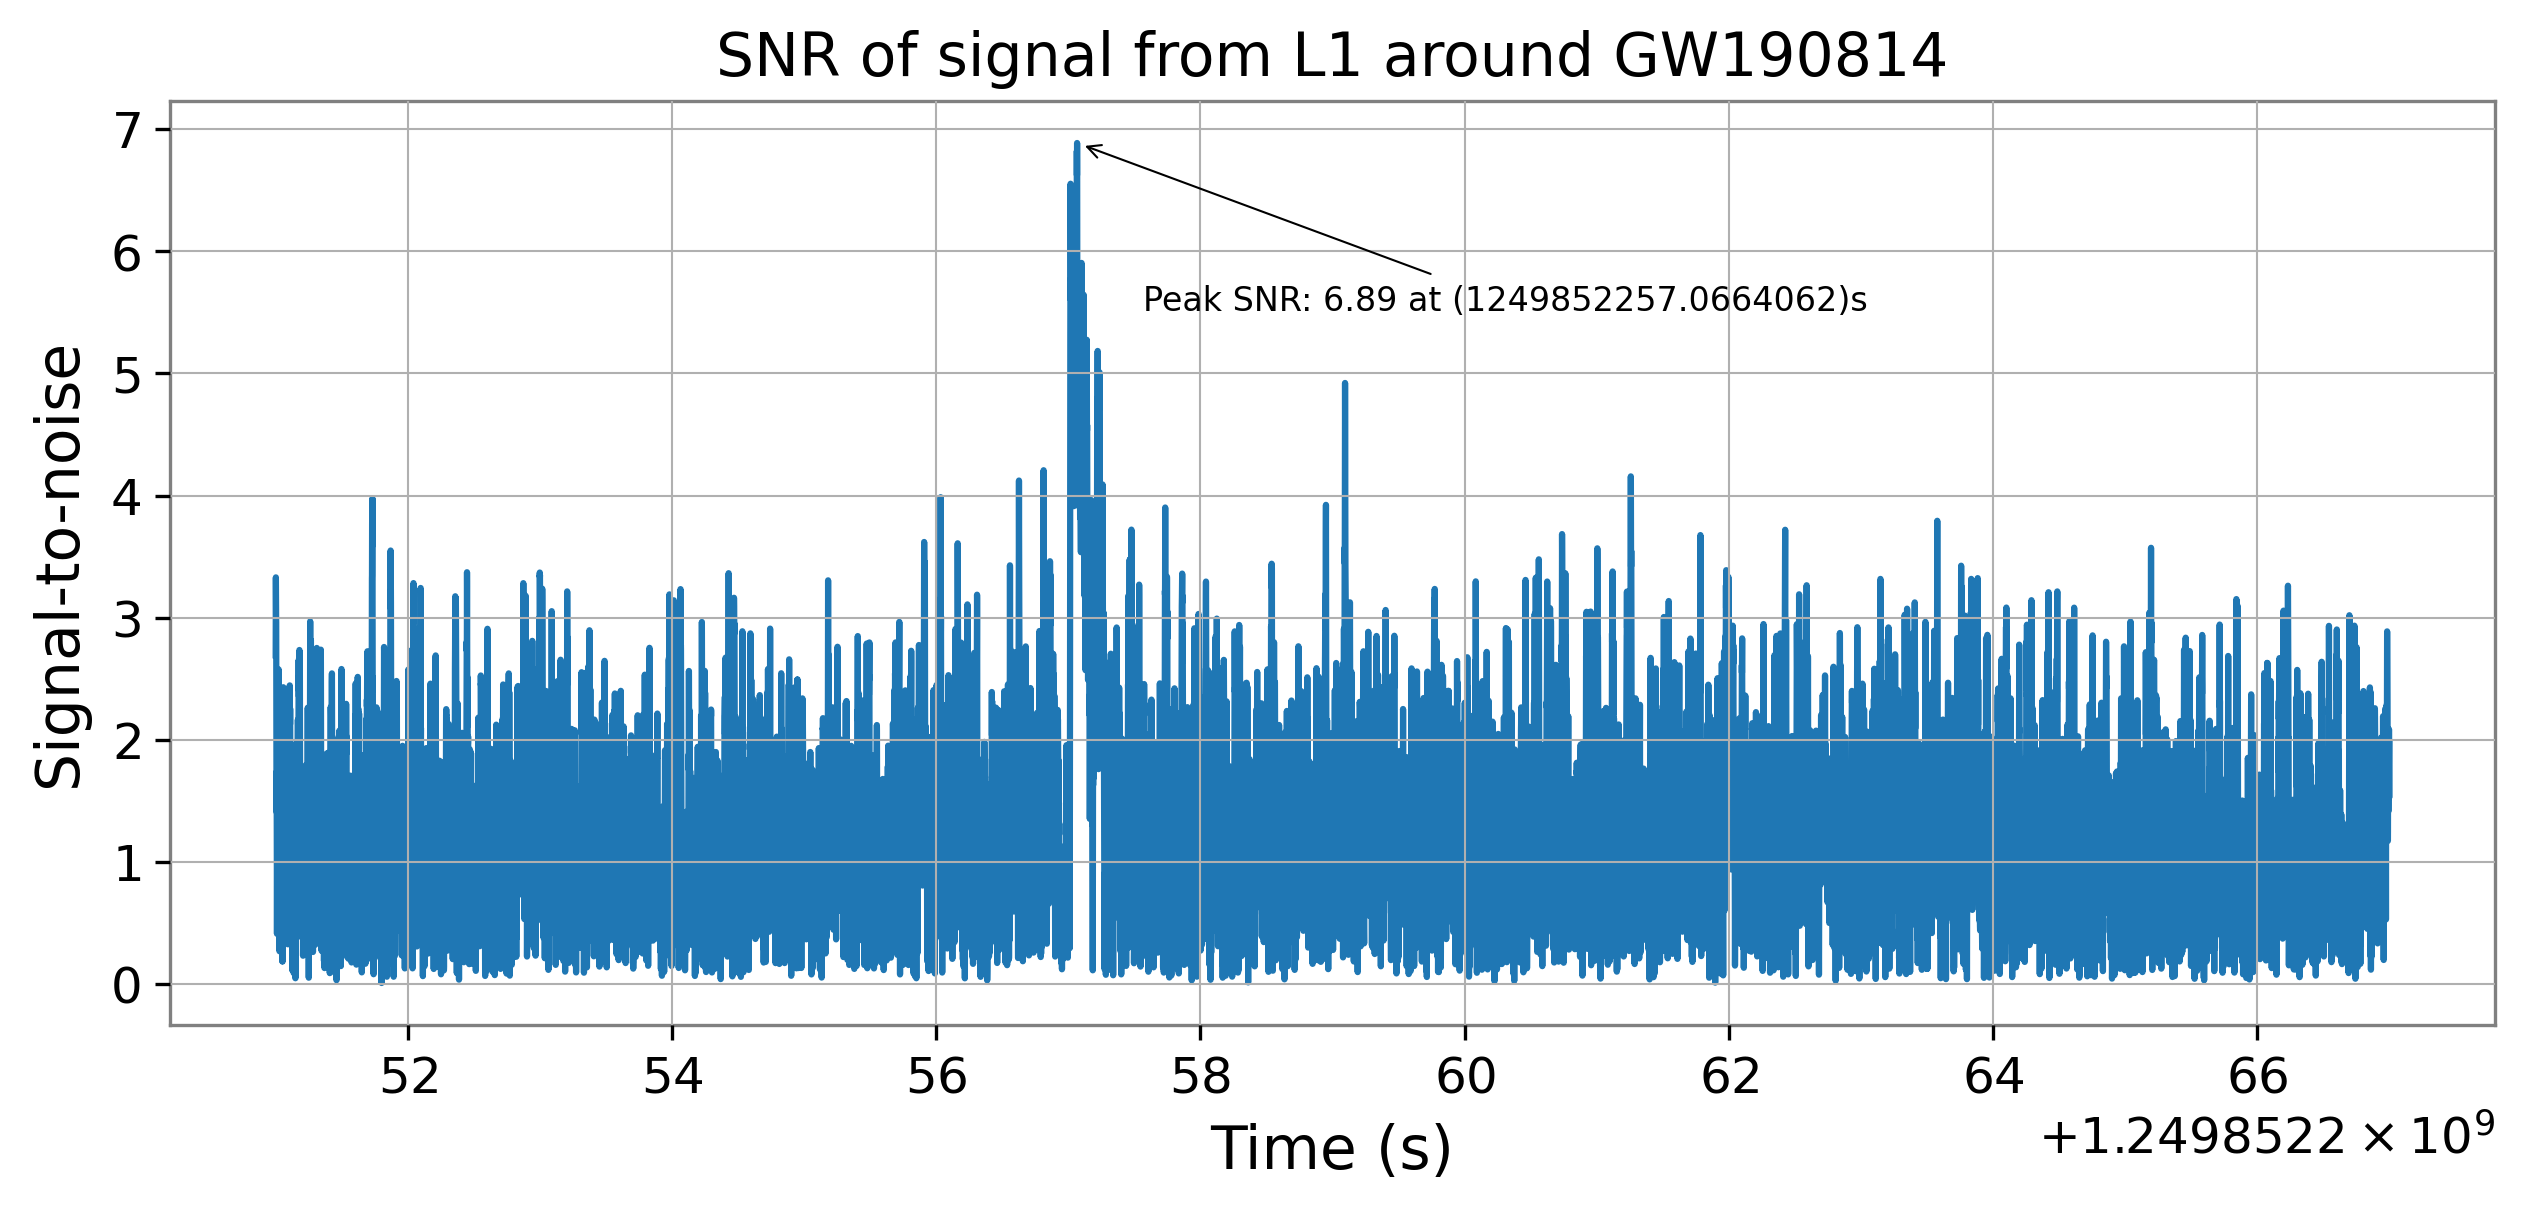
\includegraphics[width=0.78\textwidth]{GWanalysisProject_codefile/SNRplot/SNRL1GW190814.png}
            \caption{SNR from L1 detector around GW190814}
            \label{fig:GW190814SNR}
\end{figure}

\begin{figure}[h]
            \centering          
            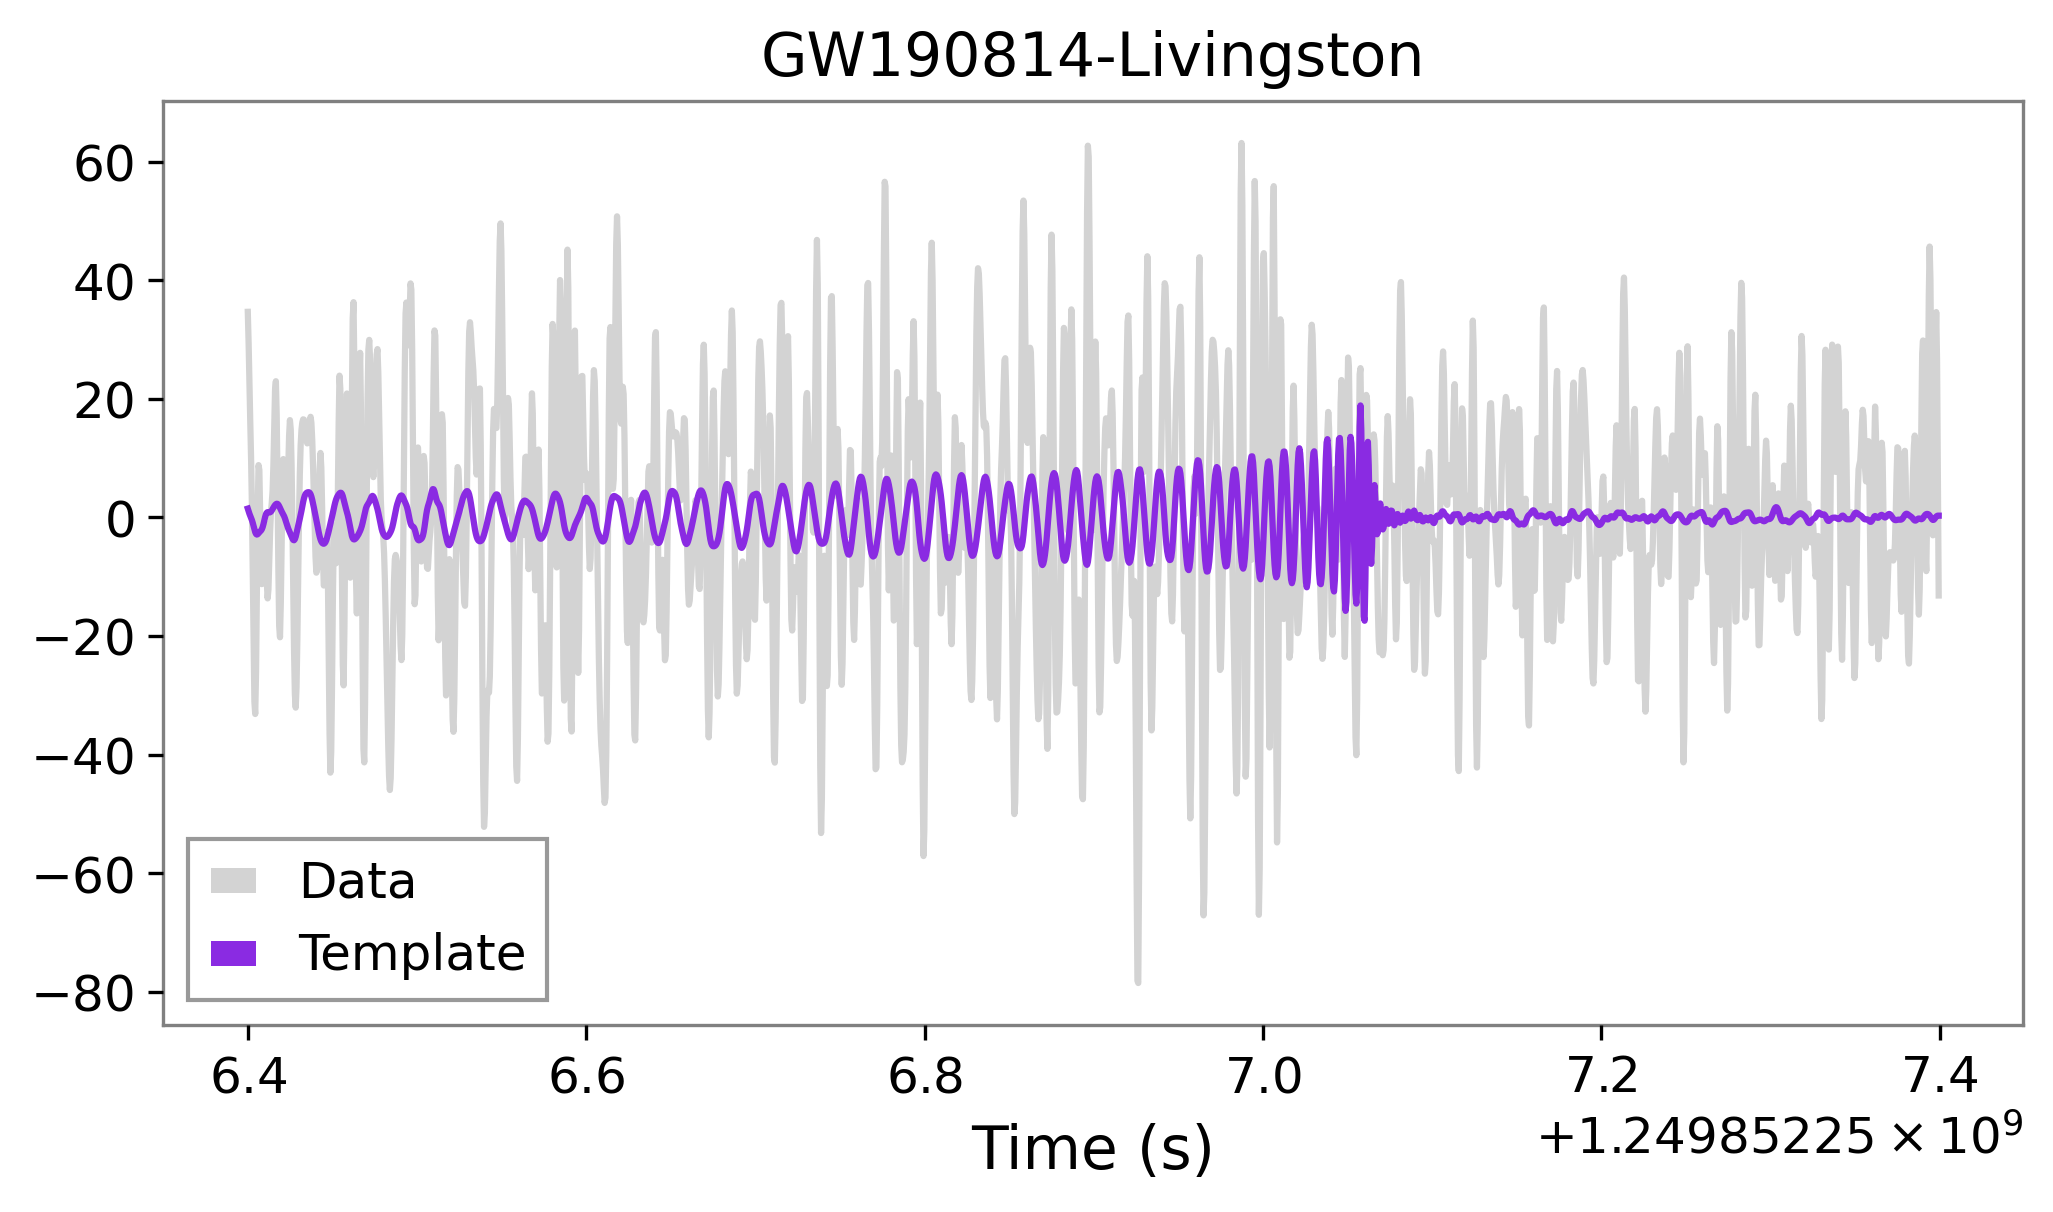
\includegraphics[width=0.75\textwidth]{GWanalysisProject_codefile/templateplot/templateL1GW190814.png}
            \caption{Whitened Template data calculated from numerical solution of GR and actual recorded data around GW190814}
            \label{fig:GW190814template}
\end{figure}

The result figure \ref{fig:GW190521template} shows the frequency evolution of the stars during the last moments of binary black hole merger and fitted it with our experimental data. The plot shows a good fit which indicates that the experimental data matches with numerical data obtained from numerical solution provided by \texttt{approximant = 'IMRPhenomPv3HM'} (see Appendix \ref{code2}) which verifies Einstein's Theory of General Relativity.

% \begin{figure}[h]
%             \centering          
%             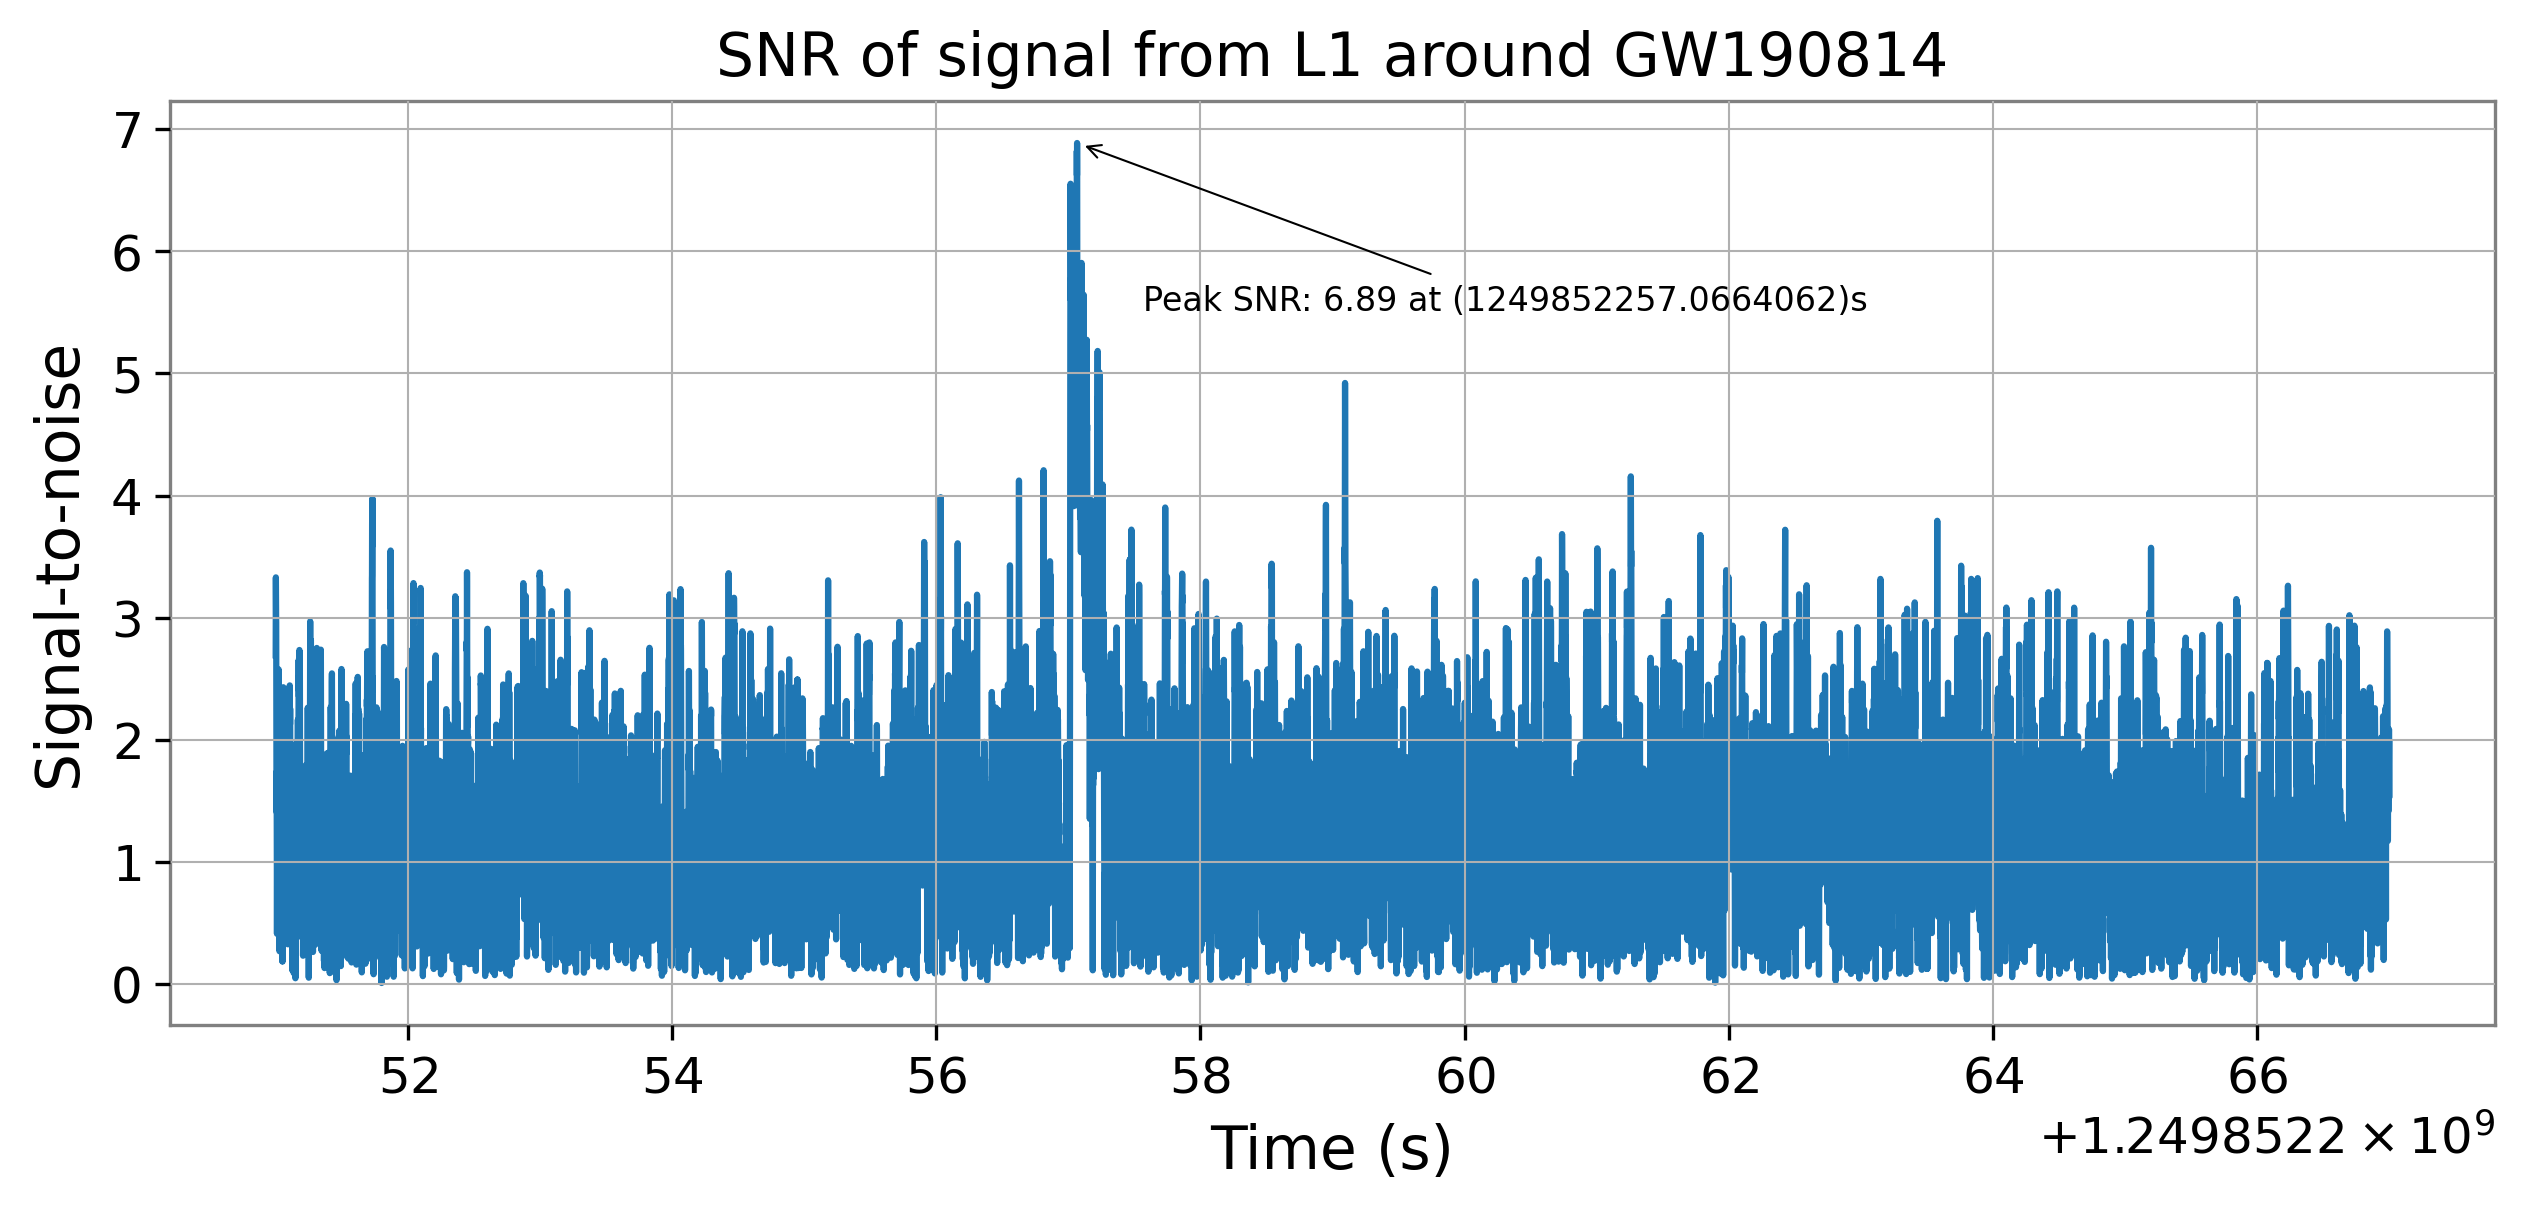
\includegraphics[width=0.75\textwidth]{GWanalysisProject_codefile/SNRplot/SNRL1GW190814.png}
%             \caption{SNR from L1 detector around GW190814}
%             \label{fig:GW190814SNR}
% \end{figure}

Similarly, the plot of the Signal-to-Noise Ratio for the signal detected by the L1 detector during incident GW190814 reveals a maximum SNR of 6.89 (Fig: \ref{fig:GW190814SNR}) at roughly 1249852257.0664062 seconds. The signal-to-noise ratio reaches its maximum value at around 58 seconds on the figure. The signal-to-noise ratio achieves an approximate maximum value of 7, confirming a robust detection of the gravitational wave event GW190814.

We generated a template plot using the \texttt{IMRPhenomPv2\_NRTidal} approximant with 2.36 $M_\odot$ for both stars and a distance of 42 Mpc, computed with a time resolution of \texttt{conditioned.delta\_t} and a 60 Hz lower frequency bound. The plot (Fig: \ref{fig:GW190814template}) shows a strong fit between the experimental data and the numerical waveform, validating Einstein's Theory of General Relativity.

% \begin{figure}[h]
%             \centering          
%             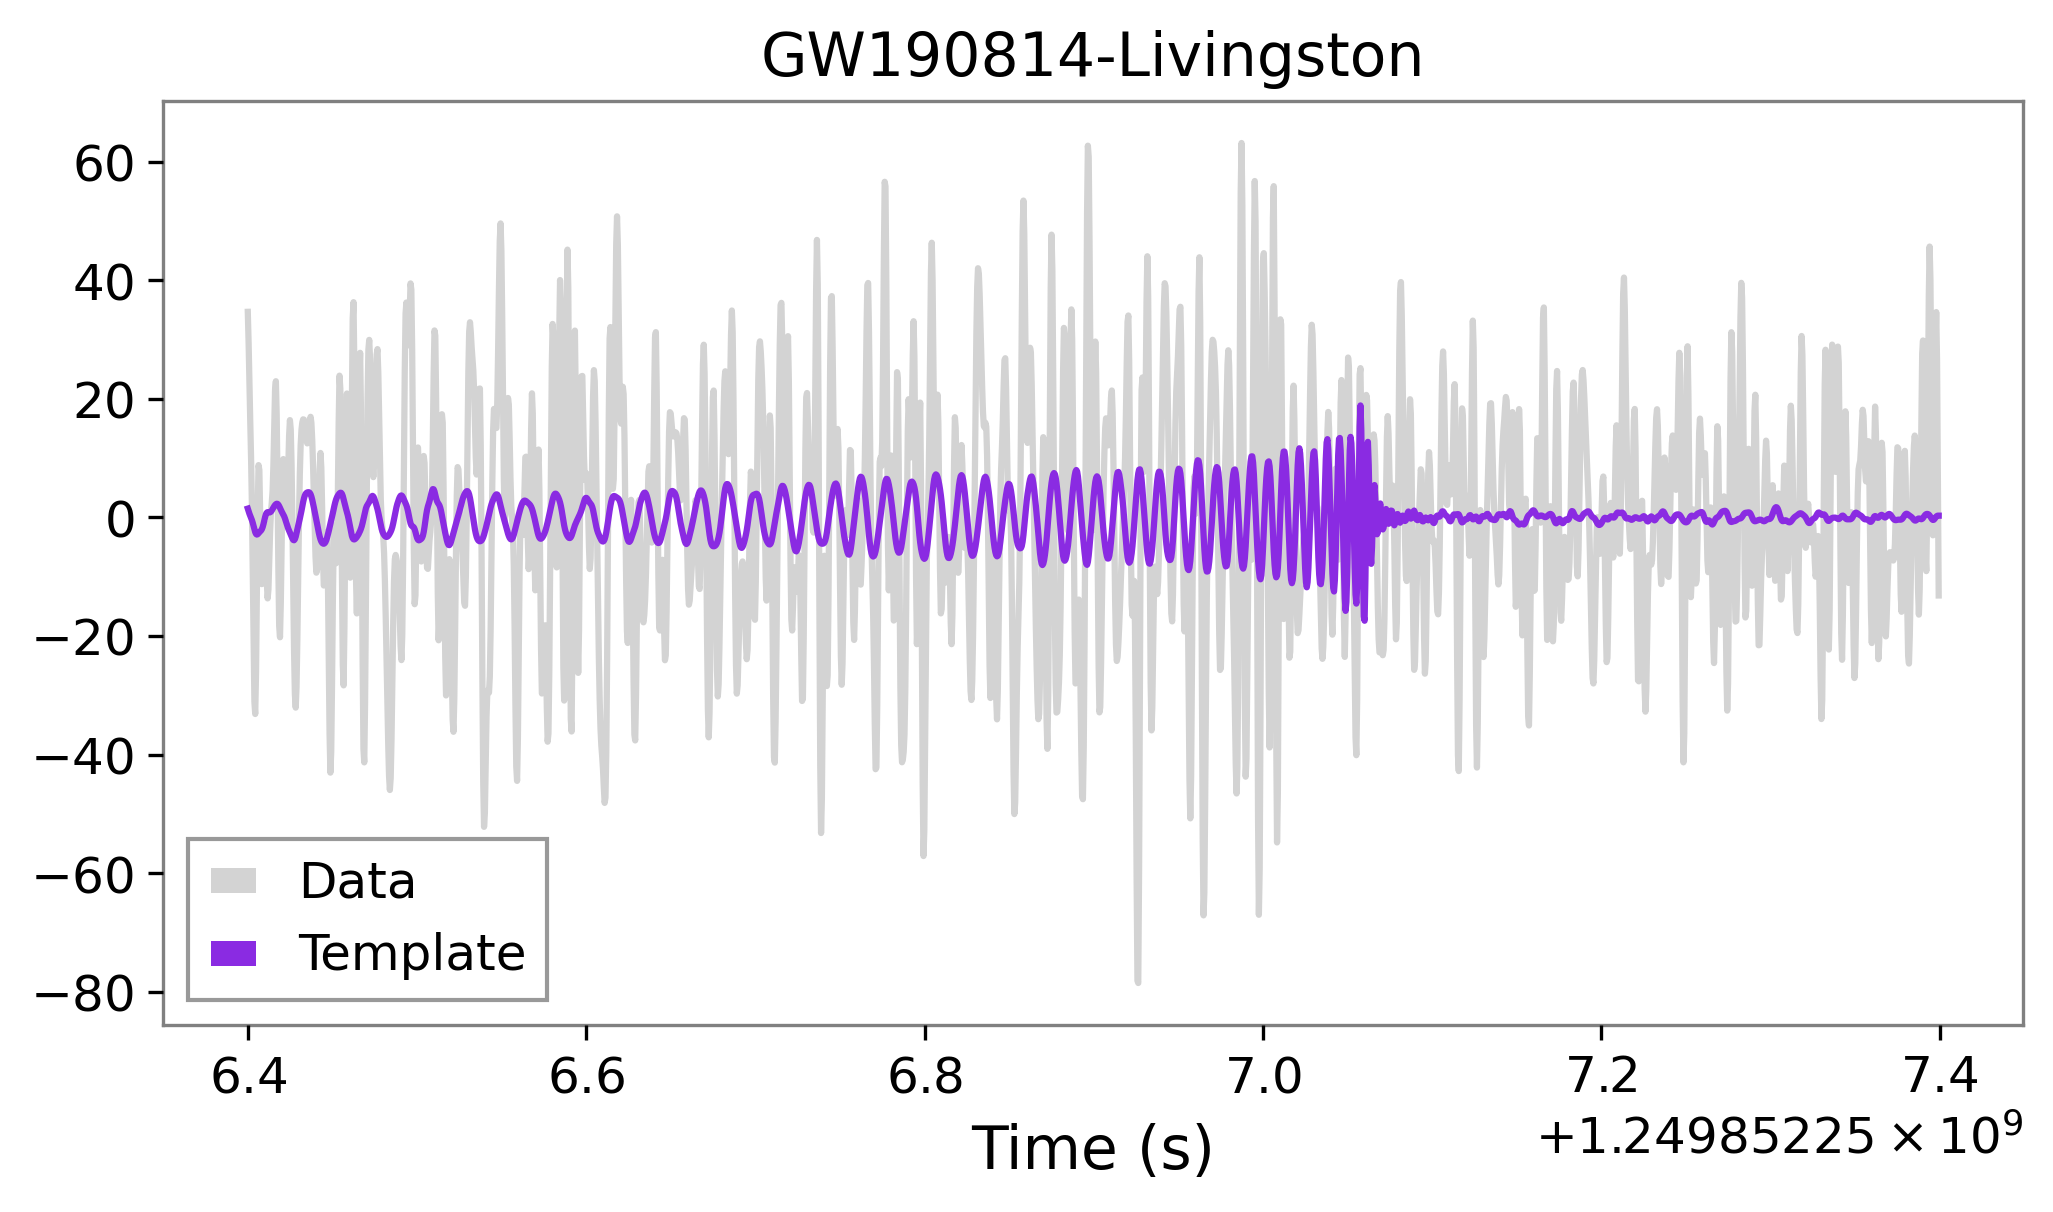
\includegraphics[width=0.75\textwidth]{GWanalysisProject_codefile/templateplot/templateL1GW190814.png}
%             \caption{Whitened Template data calculated from numerical solution of GR and actual recorded data around GW190814}
%             \label{fig:GW190814template}
% \end{figure}

Based on the comparison of gravitational wave events, including GW170817, GW190521, and GW190814, some differences and similarities between the data and the detector responses are noted. For strain data, GW170817 presents a clear chirp signal with the more prominent of the two peaks in the LIGO-Livingston data and a less noticeable chirp in the LIGO-Hanford data. On the other hand, GW190521 is characterised by relatively short and low-frequency signal mainly detected in LIGO-Livingston and LIGO-Hanford data, due to the massive black holes involved. Likewise, GW190814 has a strong chirp in LIGO-Livingston but is relatively weak in Hanford and VIRGO data. The ASD shows that LIGO-Livingston has a higher sensitivity with low strain noise than LIGO-Hanford and VIRGO for all the events detected. Higher strain noise and clear peaks at different frequencies can be observed for VIRGO which could be a sign of narrower noise sources. Further substantiation of these facts is provided by the Q-transform analysis, which indicates that GW170817 and GW190814 are characterized by distinct chirp signals in the LIGO-Livingston data, while GW190521 demonstrates a brief low-frequency signal. The Signal-to-Noise Ratio plots indicate that GW190521 and GW190814 were robustly detected, with maximum SNR values of 8.95 and 7, respectively, suggesting significant gravitational wave signals. The matching of the template fits confirms that the observed experimental results are in good agreement with the theoretical calculations based on the General Theory of Relativity by Albert Einstein.




\chapter{CONCLUSIONS AND RECOMMENDATIONS}
\onehalfspacing

\section{Conclusions}
We have analysed three gravitational wave events namely GW170817, GW190521, and GW1908\\14 employing strain data, Amplitude Spectral Density plots, Q-transform spectrograms, Signal-to-Noise Ratio analysis and template matching. 
 
%  Due to the fact that GW170817 was a binary neutron star merger, there was a strong chirp signal in the time series analysis and this was clearly evident in the LIGO-Livingston detector. This event also demonstrated LIGO detectors’ high sensitivity especially in the lower frequencies. On the other hand, GW190521 that is associated with the merger of two big black holes released a short and low frequency signal consistent with the energetic and short-lived process. Observations of the GW190814 which probably involved a binary black-hole with a higher mass ratio than the other binary black-holes showed a signal that was as long and frequent as that of neutron star and black-hole merger signals.

% The LIGO-Livingston strains recorded for GW170817 were the lowest over a broad frequency band and especially below 100 Hz, which makes the detector more sensitive to neutron star merger signals. On the other hand, both GW190521 and GW190814, which involved higher frequency emissions, brought attention to the wider noise range in the Virgo detector where noticeable tonal peaks could be observed. The sensitivity of L1 LIGO detector was better in all three events while the Virgo detector was found to have higher noise especially in the lower frequencies.

% The spectrogram of GW170817 showed the characteristic “chirp” signal, where the frequency increased as the neutron stars moved closer to merge. This signal, however, was most explicit in the L1 data. However, We found some loud instrumental noise or glitches in L1 detector. On the other hand, GW190521’s spectrogram showed a short single, low frequency centered around 60 Hz, which is suggestive of massive black hole merging. The spectrogram of GW190814 also contains the chirp like signal, but it also demonstrates the dynamics of a high mass ratio binary, which begins at the low frequencies and gradually increases to represent the merger of the binary.

%  Similarly, GW190521 had the largest peak SNR of 8.95 in the L1 detector which shows that the detector has a good efficiency of detection even if the signal is short. Conversely, the maximum SNR for GW190814 was found to be 6.89, although lower, still endorse a good detection. The template matching for both events, with numerical relativity waveforms, revealed a very good match between the experiments and the theories, thus confirming the general theory of relativity. Specifically, the waveform approximants employed – ‘IMRPhenomPv3HM’ for GW190521 and ‘IMRPhenomPv2\_NRTidal’ for GW190814, brought out the need for different models based on the mass and dynamics of merging objects.

%  A comparison of these events reveals the differences in the gravitational wave signals and the ability of the detectors to pick different types of signals. GW170817 is a relatively short binary neutron star merger signal, which is within the LIGO’s detectable frequency range at the lower end. Conversely, the higher mass black hole mergers GW190521 and GW190814 generated shorter and lower frequency signals with the GW190521 signal being difficult to detect due to its short duration and low frequency. The findings highlight the importance of multi-detector detections in covering the entire range of the gravitational waves and stress the ongoing work on the increases of the detectors’ sensitivity and the improvement of the analysis capabilities.

The comparisons revealed distinct differences based on the nature of the sources. For instance, the binary neutron star merger GW170817 produced a strong chirp signal, which was most evident in the LIGO-Livingston detector. This contrasted with GW190521, a merger of massive black holes that resulted in a short, low-frequency signal. GW190814, which likely involved a binary black hole with a higher mass ratio, exhibited a signal longer and more frequent than that of GW190521, but still different from the neutron star merger.

The comparison of strain data showed that LIGO-Livingston had the lowest noise levels, especially for GW170817, which made it more sensitive to lower frequency signals typical of neutron star mergers. On the other hand, Virgo exhibited higher noise levels, particularly noticeable in the higher frequency emissions of GW190521 and GW190814.

In comparing the spectrograms, the characteristic chirp of GW170817 was most clearly visible in the LIGO-Livingston data, despite some instrumental noise. For GW190521, the spectrogram highlighted a brief, low-frequency signal, consistent with the merger of massive black holes, while GW190814’s spectrogram captured a unique chirp-like signal indicative of a high mass ratio binary.

The SNR analysis further emphasized these differences, with GW190521 showing the highest peak SNR of 8.95, indicating robust detection despite the short signal. Although the SNR for GW190814 was lower, it still confirmed a good detection. Template matching with numerical relativity waveforms demonstrated strong correlations, validating Einstein's General Theory of Relativity. The need for different waveform approximants for these events underscored the importance of using appropriate models based on the mass and dynamics of the merging objects.

By comparing these events, We were able to identify how different gravitational wave signals and detector sensitivities affect the detection and analysis of these cosmic events. The results stress the importance of multi-detector detections to cover the full spectrum of gravitational wave signals and highlight ongoing efforts to enhance detector sensitivity and improve analysis techniques.

\section{Limitations}
The study also had some limitations that affected some of the results in the study. First, a high computational cost is another factor that prevented the authors from undertaking more complex data analyses, which would have enabled them to delve deeper into the issue at hand. The analysis was also sensitive to noise, which could lead to large errors in the results. In particular, glitches which were apparent, especially in LIGO-Livingston data during GW170817 brought significant difficulties in the correct signal analysis and interpretation of the strain data and spectrograms. In addition, the waveform templates in this paper were constructed with certain approximants and mass parameters that might not describe the full details of the events to which they were matched, which could affect the template matching. Finally, template matching was not applicable for the GW170817 event due to the problems with the parameters for the template generation and because of this, the comparative analysis for this event was limited.

\section{Recommendations For Future Work}
Future work should include SNR and template matching for the GW170817 event to provide a more complete comparative analysis across all three events, as the current study faced difficulties in adjusting parameters for template generation, limiting the scope of comparison. Additionally, further investigation is needed to explore advanced deep learning methods, such as convolutional and recurrent neural networks, to improve the detection, classification, and estimation of gravitational waves. Integrating these deep learning approaches with conventional techniques in real-time data processing could significantly enhance the speed and precision of observatory operations. Utilizing sophisticated noise reduction techniques, including machine learning algorithms, may also improve the sensitivity of detectors. Furthermore, employing Bayesian inference and machine learning to refine parameter estimates could provide deeper insights into the dynamics of binary systems. 



\newpage
\renewcommand{\bibname}{REFERENCES}
\bibliographystyle{apalike}
\addcontentsline{toc}{chapter}{References}
\bibliography{bibliography}

\appendix
\renewcommand{\thesection}{\Alph{section}.}

\chapter*{APPENDIX}
\addcontentsline{toc}{chapter}{\textbf{APPENDIX}}
\onehalfspacing


\section{Python Implementation for Strain, ASD and Qtransform plot}
\label{code1}

\begin{lstlisting}[language=Python, caption=Preprocessing Implementation in python]
""
Written By
    Shivaji Chaulagain
""
from gwosc import datasets
from gwpy.timeseries import TimeSeries, TimeSeriesDict
from matplotlib import pyplot as plt
from pycbc.waveform import get_td_waveform, fd_approximants
import numpy as np
from scipy import signal as sc

class GWanalysis:
  def __init__(self, eventname, duration):
    self.eventname = eventname
    self.duration = duration
    self.gps = datasets.event_gps(eventname)
    self.segment = (int(self.gps)-self.duration/2, int(self.gps)+self.duration/2)
    self.ldata = TimeSeries.fetch_open_data("L1", *self.segment, cache=True)
    self.hdata = TimeSeries.fetch_open_data("H1", *self.segment, cache=True)
    self.vdata = TimeSeries.fetch_open_data("V1", *self.segment, cache=True)
  # plot strain data of given duration.
  def straindataplot(self):
    combined = TimeSeriesDict()
    combined['L1'] = self.ldata
    combined['H1'] = self.hdata
    combined['V1'] = self.vdata
    plot = combined.plot(figsize=(12, 10), separate=True, sharex=True)
    ax1, ax2, ax3 = plot.axes
    ax1.set_title(f'LIGO-Hanford-Virgo strain data around {self.eventname} of duration {self.duration}s')
    ax1.set_ylabel('Amplitude [strain]', y=-0.5)
    ax1.lines[0].set_color('blue')
    ax2.lines[0].set_color('green')
    ax3.lines[0].set_color('red')
    ax1.legend()
    ax2.legend()
    ax3.legend()
    ax2.set_ylabel('')
    ax3.set_ylabel('')
    plot.savefig(f'{self.eventname}strain.png')
  # plot the Amplitude Spectral density. More duration(s) better the resolution of frequency component
  def asdplot(self, fftlength=4, method="median"):
    asdl = self.ldata.asd(fftlength=fftlength, method="median")
    asdh = self.hdata.asd(fftlength=fftlength, method="median")
    asdv = self.vdata.asd(fftlength=fftlength, method="median")
    lasd = asdl.plot()
    ax = lasd.gca()
    ax.set_xlim(10, 1400)
    ax.set_ylim(1e-24, 1e-20)
    ax.plot(asdh, label='LIGO-Hanford', color='gwpy:ligo-hanford')
    ax.plot(asdv, label='Virgo', color='gwpy:virgo')

    lline = ax.lines[0]
    lline.set_color('gwpy:ligo-livingston')  
    lline.set_label('LIGO-Livingston')

    ax.set_ylabel(r'Strain noise [$1/\sqrt{\mathrm{Hz}}$]')
    ax.set_title(f'ASD of each detector around {self.eventname}')
    ax.legend(fontsize=7,loc='lower left')
    plt.savefig(f'{self.eventname}asd.png', dpi=300, bbox_inches='tight')
  # q-transform. I have kept duration of 32 second for signal
  def qtransformplot(self, franges, qranges, outsegs=None):
    if outsegs is not None:
        o1, o2 = outsegs
    ldata = TimeSeries.fetch_open_data("L1", int(self.gps)-30, int(self.gps)+2, cache=True)
    hdata = TimeSeries.fetch_open_data("H1", int(self.gps)-30, int(self.gps)+2, cache=True)
    vdata = TimeSeries.fetch_open_data("V1", int(self.gps)-30, int(self.gps)+2, cache=True)
    if outsegs is None:
        lq = ldata.q_transform(frange=franges, qrange=qranges)
        hq = hdata.q_transform(frange=franges, qrange=qranges)
        vq = vdata.q_transform(frange=franges, qrange=qranges)
    else:
        lq = ldata.q_transform(frange=franges, qrange=qranges, outseg=(self.gps-o1, self.gps+o2))
        hq = hdata.q_transform(frange=franges, qrange=qranges, outseg=(self.gps-o1, self.gps+o2))
        vq = vdata.q_transform(frange=franges, qrange=qranges, outseg=(self.gps-o1, self.gps+o2))
    plot, axes = plt.subplots(nrows=3, sharex=True, figsize=(5, 10))
    tax, qax, qax2 = axes
    tax.imshow(lq)
    qax.imshow(hq)
    qax2.imshow(vq)
    tax.set_title(f"Q-transform around {self.eventname}")
    tax.set_ylabel('Frequency [Hz]', y=-0.5)
    qax.set_ylabel('')
    qax2.set_ylabel('')
    qax2.set_xlabel('Time[seconds]')
    tax.set_yscale('log')
    qax.set_yscale('log')
    qax2.set_yscale('log')
    tick_positions = np.arange(-o1, o2, 0.4)
    # tax.set_xticklabels([])
    # qax.set_xticklabels([])
    # qax2.set_xticklabels([])
    tax.set_xticklabels([round(pos,2) for pos in tick_positions])
    qax.set_xticklabels([round(pos,2) for pos in tick_positions])
    qax2.set_xticklabels([round(pos,2) for pos in tick_positions])
    # show the detector name in plot
    tax.text(0.05, 0.95, 'LIGO-Livingston', transform=tax.transAxes, fontsize=7, verticalalignment='top', color='white')
    qax.text(0.05, 0.95, 'LIGO-Hanford', transform=qax.transAxes, fontsize=7, verticalalignment='top', color='white')
    qax2.text(0.05, 0.95, 'Virgo', transform=qax2.transAxes, fontsize=7, verticalalignment='top', color='white')
    # hide gid
    tax.grid(False)
    qax.grid(False)
    qax2.grid(False)
    tax.colorbar(clim = (0,20),label='Normalised energy')
    qax.colorbar(clim = (0,20))
    qax2.colorbar(clim = (0,20))

    plt.savefig(f'{self.eventname}_qtransform.png', dpi=300, bbox_inches='tight')
    
\end{lstlisting}
\newpage
\section{Python Implementation for Waveform Generation (Template)}
\label{code2}

For information about the conditioned variable, what the below code is and how it is obtained and the remaining code for whitening and template generation, see the following references in the gw-odw2023 GitHub repository: \url{https://github.com/gw-odw/odw-2023/blob/main/Tutorials/Day_2/Tuto_2.2_Matched_Filtering_In_action.ipynb}. Furthermore, about my work, see my github repository: \url{https://github.com/Shivaji-137}
\subsection{GW190521}
\begin{lstlisting}
conditioned = strain.crop(2, 2) #obtained from strain data
from pycbc.waveform import get_td_waveform
hp, hc = get_td_waveform(approximant="IMRPhenomPv3HM",
                     mass1=90,
                     mass2= 65,
                     distance = 4600,
                     delta_t=conditioned.delta_t,
                     f_lower=20)

# Resize the vector to match our data
hp.resize(len(conditioned))
\end{lstlisting}
\subsection{GW190814}
\begin{lstlisting}
from pycbc.waveform import get_td_waveform
hp, hc = get_td_waveform(approximant="IMRPhenomPv2_NRTidal",
                     mass1=2.36,
                     mass2= 2.36,
                     distance = 42,
                     delta_t=conditioned.delta_t,
                     f_lower=60)

# Resize the vector to match our data
hp.resize(len(conditioned))
\end{lstlisting}
 





\end{document}